\documentclass[a4paper, 12pt]{report}
\usepackage[utf8]{inputenc}
\usepackage[italian]{babel}
\usepackage{amsmath, amssymb, amsthm}
\usepackage{graphicx}
\usepackage{geometry}
\usepackage{booktabs}
\usepackage{hyperref}
\usepackage{listings}
\usepackage{xcolor}
\usepackage{float}
\usepackage{caption}

\geometry{a4paper, margin=2cm}

% Configurazione per il codice Python
\definecolor{codegreen}{rgb}{0,0.6,0}
\definecolor{codegray}{rgb}{0.5,0.5,0.5}
\definecolor{codepurple}{rgb}{0.58,0,0.82}
\definecolor{backcolour}{rgb}{0.95,0.95,0.92}
\lstdefinestyle{mystyle}{
    backgroundcolor=\color{backcolour},   
    commentstyle=\color{codegreen},
    keywordstyle=\color{magenta},
    numberstyle=\tiny\color{codegray},
    stringstyle=\color{codepurple},
    basicstyle=\ttfamily\footnotesize,
    breakatwhitespace=false,         
    breaklines=true,                 
    captionpos=b,                    
    keepspaces=true,                 
    numbers=left,                    
    numbersep=5pt,                  
    showspaces=false,                
    showstringspaces=false,
    showtabs=false,                  
    tabsize=2
}
\lstset{style=mystyle}

\title{\Huge\textbf{Progetto 1 - Metodi del Calcolo Scientifico}\\ \vspace{0.5cm} \Large \textbf{Libreria per sistemi lineari iterativi}}
\author{\textbf{Nomi Componenti Gruppo} \\ Andrea Mauri : 945327 \\ Luca Rossini: 900230\\ Francesco Sormani: 894552}
\date{Anno Accademico 2025-2026}

\begin{document}

\maketitle

\tableofcontents
\newpage

\chapter{Introduzione}
\section{Obiettivo del Progetto}
Il presente documento relaziona il lavoro svolto per la progettazione, sviluppo e analisi dei risultati di una libreria software dedicata alla risoluzione di sistemi lineari $Ax = b$ attraverso l'utilizzo di metodi iterativi. In conformità con le specifiche di progetto, la libreria è stata concepita esclusivamente per operare su matrici simmetriche e definite positive.

\noindent Gli algoritmi implementati sono i seguenti:
\begin{enumerate}
    \item Metodo di Jacobi;
    \item Metodo di Gauß-Seidel;
    \item Metodo del Gradiente;
    \item Metodo del Gradiente Coniugato.
\end{enumerate}

\section{Scelte Implementative}
Il linguaggio scelto per lo sviluppo è \textbf{Python}, affiancato dalle librerie \texttt{NumPy} e \texttt{SciPy}.
\subsection{Supporto di matrici sparse}
Per la gestione dei dati è stato utilizzato il modulo \texttt{scipy.sparse}, essenziale per manipolare con efficienza le matrici in formato \texttt{.mtx}. Abbiamo scelto di operare principalmente sul formato CSR (\textit{Compressed Sparse Row}), una scelta dettata dalla natura stessa dei metodi iterativi.

\noindent L'adozione del CSR offre vantaggi significativi sia in termini di memoria che di prestazioni:
\begin{itemize}
    \item \textbf{Efficienza di memoria}: Invece di allocare spazio per ogni singola cella della matrice, il CSR memorizza esclusivamente i valori non-zero. Questo permette di gestire sistemi lineari di enormi dimensioni che altrimenti saturerebbero la RAM.
    \item \textbf{Accesso rapido per riga}: La struttura del CSR, basata sui tre vettori \textit{data}, \textit{indices} e \textit{indptr}, è progettata per rendere istantaneo il recupero di un'intera riga della matrice. Poiché l'operazione dominante nei nostri algoritmi è il prodotto matrice-vettore (o la risoluzione di sistemi triangolari), poter scorrere velocemente gli elementi di una riga senza dover passare tra locazioni di memoria distanti garantisce un utilizzo ottimale della cache del processore.
\end{itemize}

È fondamentale precisare che l'apporto di \texttt{SciPy} è stato limitato alle sole operazioni di base (somme, prodotti, calcolo di norme), garantendo il pieno rispetto dei vincoli didattici ed evitando l'uso di funzioni di risoluzione predefinite per i sistemi lineari.

\subsection{Criterio di arresto}

La consegna richiede che i metodi iterativi si arrestino al soddisfacimento della seguente condizione sulla norma relativa del residuo:
\begin{equation} \label{eq:consegna_prof}
    \frac{\|Ax^{(k)} - b\|_2}{\|b\|_2} < \text{tol}
\end{equation}

\noindent Nella nostra libreria abbiamo scelto di formulare il controllo di convergenza utilizzando la norma del vettore residuo $r^{(k)}$ calcolato ad ogni passo:
\begin{equation} \label{eq:nostra_formula}
    \frac{\|r^{(k)}\|_2}{\|b\|_2} < \text{tol}
\end{equation}
Questa scelta garantisce una perfetta equivalenza matematica con la formula (\ref{eq:consegna_prof}). Per definizione di residuo, si ha infatti $r^{(k)} = b - Ax^{(k)}$, il che implica:
$$\|r^{(k)}\|_2 = \|b - Ax^{(k)}\|_2 = \|-(Ax^{(k)} - b)\|_2 = \|Ax^{(k)} - b\|_2$$

\noindent Il vantaggio principale di questo approccio è puramente prestazionale, infatti in metodi come il Gradiente o il Gradiente Coniugato il residuo $r^{(k)}$ è una variabile di stato fondamentale che viene aggiornata iterativamente o ricalcolata per determinare la direzione di discesa. Utilizzando direttamente $\|r^{(k)}\|$, evitiamo di dover ricalcolare il prodotto matrice-vettore $Ax^{(k)}$ e la successiva sottrazione solo per eseguire il test di arresto. Questo accorgimento permette di diminuire il numero di prodotti matrice-vettore per iterazione in molti dei metodi implementati, portando a un risparmio di tempo significativo senza alcun impatto sulla precisione numerica.


\subsection{Validazione dei Parametri}
La libreria esegue una fase di validazione per assicurare che i dati in ingresso siano coerenti con le ipotesi teoriche degli algoritmi. Questo approccio previene errori a runtime e garantisce l'affidabilità dei risultati. I controlli effettuati includono:
\begin{itemize}
    \item \textbf{Verifica strutturale}: si accerta che la matrice $A$ sia quadrata e che il vettore $b$ abbia dimensioni compatibili per l'operazione $Ax = b$.
    \item \textbf{Vincolo di sparsità}: viene verificato che la matrice appartenga al modulo \texttt{scipy.sparse}, forzando l'uso di strutture dati efficienti.
    \item \textbf{Controllo SPD (Simmetrica e definita positiva)}: trattandosi di metodi ottimizzati per matrici SPD, la libreria verifica la simmetria ($A = A^T$) e la positività definita. Per quest'ultima, si utilizza la decomposizione di Cholesky su sistemi piccoli ($n \le 500$) o il calcolo dell'autovalore minimo per matrici di dimensioni superiori.
    \item \textbf{Parametri di controllo}: viene imposto un limite minimo di 20.000 per il parametro \texttt{maxIter}, assicurando che i metodi abbiano un margine sufficiente per raggiungere la convergenza richiesta.
\end{itemize}

\subsection{Procedura di Validazione}
La correttezza degli algoritmi è stata verificata attraverso un protocollo di validazione diviso in quattro fasi:
\begin{enumerate}
    \item \textbf{Definizione della verità}: si fissa un vettore soluzione esatta $x = [1, 1, \dots, 1]^T$.
    \item \textbf{Costruzione del sistema}: dato $x$ e una matrice SPD $A$, si calcola $b = Ax$.
    \item \textbf{Risoluzione numerica}: si applicano i metodi iterativi per ricavare la soluzione approssimata $\hat{x}$.
    \item \textbf{Analisi dell'errore}: si confronta $\hat{x}$ con $x$ calcolando l'errore relativo in norma euclidea: $E_{rel} = \frac{\|\hat{x} - x\|_2}{\|x\|_2}$.
\end{enumerate}
Questo test è stato condotto su quattro differenti matrici di prova (\texttt{spa1, spa2, vem1, vem2}) permettendo di variare la tolleranza tra $10^{-4}$,$10^{-6}$,$10^{-8}$  e $10^{-10}$, assicurando così una copertura dei possibili scenari d'uso.


\chapter{Struttura del Progetto}
L'implementazione del progetto è stata organizzata in modo modulare, separando la libreria di calcolo dai servizi di utilità e gestione. Di seguito viene mostrata la gerarchia dei file presenti nella repository.

\begin{verbatim}
prog1bis-metodi
|-- linear_iterative_solvers_lib
|   |-- pyproject.toml
|   |-- src
|   |   |-- linear_iterative_solvers
|   |   |   |-- __init__.py
|   |   |   |-- base.py
|   |   |   |-- conjugate_gradient.py
|   |   |   |-- gauss_seidel.py
|   |   |   |-- gradient.py
|   |   |   |-- jacobi.py
|-- services
|   |-- matrix.py
|   |-- parser.py
|   |-- print.py
|   |-- plot.py
|   |-- utils.py
|-- main.py
|-- requirements.txt
\end{verbatim}

\noindent La radice del progetto è suddivisa in componenti logiche ben definite:
\begin{itemize}
    \item \texttt{linear\_iterative\_solvers\_lib/}: libreria Python contenente le implementazioni degli algoritmi. La libreria segue la struttura standard per il packaging e possiede anche una classe base astratta \texttt{base.py} che incapsula la logica di validazione delle matrici.
    \item \texttt{services/}: moduli di supporto per il caricamento, il parsing dei parametri, la visualizzazione dei risultati e la creazione dei grafici.
    \item \texttt{main.py}: punto d'ingresso principale del progetto.
\end{itemize}

\section{Moduli di Servizio}
Per mantenere elevata la manutenibilità, le operazioni accessorie sono isolate in moduli specifici:
\begin{itemize}
    \item \textbf{\texttt{parser.py}}: gestisce la configurazione dinamica dell'esecuzione tramite interfaccia a riga di comando.
    \item \textbf{\texttt{matrix.py} e \texttt{utils.py}}: gestiscono il caricamento delle matrici sparse e forniscono funzioni di utilità generale.
    \item \textbf{\texttt{print.py}}: formatta e visualizza i risultati delle iterazioni a console in modo leggibile.
    \item \textbf{\texttt{plot.py}}: genera i grafici per la visualizzazione dei risultati ottenuti e li salva nella cartella \texttt{plots/}.
\end{itemize}


\chapter{Metodi Iterativi Implementati}
In questa sezione vengono analizzati nel dettaglio i quattro metodi iterativi implementati nella libreria. Per ognuno di essi viene fornita una descrizione teorica, lo schema delle proprietà principali, lo pseudocodice logico e le specifiche scelte implementative adottate per massimizzare le prestazioni.

\section{Metodo di Jacobi}

Il metodo di Jacobi è un metodo iterativo stazionario per la risoluzione
di sistemi lineari $A\mathbf{x} = \mathbf{b}$, con $A \in \mathbb{R}^{n
\times n}$ simmetrica e definita positiva.

\subsection*{Idea: splitting e punto fisso}

L'idea fondamentale è decomporre la matrice $A$ nella forma $A = D - N$,
dove $D$ è la matrice diagonale di $A$ e $N$ contiene le entrate
fuori diagonale cambiate di segno. Sostituendo nel sistema $A\mathbf{x} =
\mathbf{b}$ si ottiene:
\[
    (D - N)\mathbf{x} = \mathbf{b}
    \implies
    D\mathbf{x} = N\mathbf{x} + \mathbf{b}
    \implies
    \mathbf{x} = D^{-1}N\mathbf{x} + D^{-1}\mathbf{b}.
\]
La soluzione esatta $\mathbf{x}^*$ soddisfa questa equazione, infatti è un
punto fisso della funzione $f(\mathbf{x}) = D^{-1}N\mathbf{x} +
D^{-1}\mathbf{b}$. Questo giustifica la costruzione dell'iterazione: si
parte da $\mathbf{x}^{(0)} = \mathbf{0}$ e si applica $f$ ripetutamente,
\[
    \mathbf{x}^{(k+1)} = D^{-1}N\,\mathbf{x}^{(k)} + D^{-1}\mathbf{b}.
    \tag{Jacobi}
\]

\subsection*{Riscrittura tramite residuo}

Introduciamo il residuo all'iterazione $k$:
\[
    \mathbf{r}^{(k)} = \mathbf{b} - A\mathbf{x}^{(k)}.
\]
Il residuo misura quanto $\mathbf{x}^{(k)}$ "sbaglia" il sistema: vale
$\mathbf{r}^{(k)} = \mathbf{0}$ se e solo se $\mathbf{x}^{(k)}$ è la
soluzione esatta. Aggiungendo e sottraendo $\mathbf{x}^{(k)}$ alla formula
(Jacobi) e usando $A = D - N$ si verifica che:
\[
    \mathbf{x}^{(k+1)}
    = \mathbf{x}^{(k)} + D^{-1}\underbrace{\left(\mathbf{b} -
    A\mathbf{x}^{(k)}\right)}_{\mathbf{r}^{(k)}}
    = \mathbf{x}^{(k)} + D^{-1}\mathbf{r}^{(k)}.
\]
Le due scritture sono algebricamente equivalenti. La seconda è più
conveniente in implementazione dato che il termine $D^{-1}\mathbf{r}^{(k)}$
rappresenta la correzione da applicare all'iterata corrente,
calcolabile con una semplice divisione vettore per vettore.

\subsection*{Implementazione efficiente}

Sfruttando la sparsità di $A$ e la struttura diagonale di $D$, ogni
iterazione del metodo si riduce a tre operazioni vettoriali di costo
$\mathcal{O}(\mathrm{nnz})$. Ad ogni passo $k$, avendo già disponibile
il residuo $\mathbf{r}^{(k-1)} = \mathbf{b} - A\mathbf{x}^{(k-1)}$
calcolato all'iterazione precedente:
\begin{enumerate}
    \item \textbf{Correzione:}
          $\mathbf{x}^{(k)} = \mathbf{x}^{(k-1)} + \mathbf{r}^{(k-1)}
          \slash \mathbf{d}$\quad
          (\texttt{x = x + r / d}),
          dove $\mathbf{d}$ è il vettore delle entrate diagonali.
    \item \textbf{Prodotto sparso:}
          $\mathbf{Rx} = R\,\mathbf{x}^{(k)}$\quad
          (\texttt{Rx = R @ x}),
          dove $R = A - D$ è la matrice di scarto, contenente solo le
          entrate fuori diagonale.
    \item \textbf{Aggiornamento del residuo:}
          $\mathbf{r}^{(k)} = \mathbf{b} - \mathbf{Rx} -
          \mathbf{d}\mathbf{x}^{(k)}$\quad
          (\texttt{r = b - Rx - d * x}),
          che corrisponde a $\mathbf{b} - A\mathbf{x}^{(k)}$ spezzato
          come $\mathbf{b} - R\mathbf{x}^{(k)} - d\mathbf{x}^{(k)}$,
          pronto per la prossima iterazione.
\end{enumerate}
In questo modo si evita sia la costruzione esplicita di $D^{-1}$ come
matrice $n \times n$, sia il prodotto matrice-vettore denso, sfruttando
la rappresentazione sparsa di $A$.
\subsection*{Criterio di arresto e convergenza}

Il metodo si arresta quando il residuo relativo scende sotto una
tolleranza $\tau$ fissata dall'utente:
\[
    \frac{\|\mathbf{r}^{(k)}\|}{\|\mathbf{b}\|} < \tau,
\]
oppure quando il numero di iterazioni supera \texttt{maxIter}$= 20000$ (oppure la cifra inserita dall'utente).
La convergenza del metodo è garantita se il raggio spettrale della
matrice di iterazione $B = D^{-1}N$ soddisfa $\rho(B) < 1$; condizione
sufficiente è che $A$ sia a dominanza diagonale stretta per righe.
Nelle implementazioni pratiche non si attende la convergenza completa in quanto
il metodo si arresta quando il residuo relativo scende sotto la
tolleranza $\tau$ scelta dall'utente, oppure al raggiungimento di
\texttt{maxIter} iterazioni segnalando la mancata convergenza.
\subsection*{Pseudocodice}
\begin{verbatim}
Jacobi(A, b, tol, max_iter)

1.  Inizializza x = vettore nullo
2.  Estrai diagonale d = diagonal(A)
3.  Pre-calcola R = A - diags(d)
4.  Calcola norma_b = norma(b)
5.  Inizializza residuo r = b
6.  Calcola errore = norma(r) / norma_b

7.  WHILE (errore > tol) AND (k < max_iter):
8.      x = x + (r / d)                     // Aggiornamento della soluzione
9.      Rx = R * x                          // Prodotto matrice vettore
10.     r = b - Rx - (d * x)                // Nuovo residuo (b - Ax)
11.     errore = norma(r) / norma_b         // Calcolo errore relativo
12.     k = k + 1
13. END

14. return x, k, errore
\end{verbatim}
\section{Metodo di Gauss-Seidel}

Il metodo di Gauss-Seidel è un metodo iterativo stazionario per la
risoluzione di sistemi lineari $A\mathbf{x} = \mathbf{b}$, con
$A \in \mathbb{R}^{n \times n}$ simmetrica e definita positiva.

\subsection*{Idea: splitting e sistema triangolare}

L'idea fondamentale è decomporre la matrice $A$ come:
\[
    A = L + U,
\]
dove $L$ è la parte triangolare inferiore di $A$ (diagonale inclusa)
e $U$ è la parte strettamente triangolare superiore. Sostituendo nel
sistema $A\mathbf{x} = \mathbf{b}$ si ottiene la formula dell'iterazione:
\[
    L\,\mathbf{x}^{(k)} = \mathbf{b} - U\,\mathbf{x}^{(k-1)}.
    \tag{Gauss-Seidel}
\]
Il membro destro è noto (costruito con la $x$ dell'iterata precedente),
mentre il membro sinistro è un sistema triangolare inferiore in
$\mathbf{x}^{(k)}$, risolvibile tramite \emph{forward substitution}.
La soluzione esatta $\mathbf{x}^*$ è un punto fisso di questa
iterazione.

\subsection*{Forward substitution}

Risolvere $L\mathbf{x}^{(k)} = \mathbf{c}$, con
$\mathbf{c} = \mathbf{b} - U\mathbf{x}^{(k-1)}$, significa ricavare
le componenti di $\mathbf{x}^{(k)}$ una per volta dall'alto verso il
basso. La $i$-esima componente si calcola come:
\[
    x_i^{(k)} = \frac{1}{L_{ii}}
    \left( c_i - L_i \cdot \mathbf{x}^{(k)} \right),
    \qquad i = 1, \ldots, n,
\]
dove $L_i$ denota la $i$-esima riga di $L$ ristretta alle colonne
$j < i$. Poiché quando si calcola $x_i^{(k)}$ tutte le componenti
$x_1^{(k)}, \ldots, x_{i-1}^{(k)}$ sono già disponibili, si usano
immediatamente i valori nuovi appena calcolati nella stessa iterazione.

\subsection*{Riscrittura tramite residuo}

Introduciamo il residuo all'iterazione $k$:
\[
    \mathbf{r}^{(k)} = \mathbf{b} - A\mathbf{x}^{(k)}
    = \mathbf{b} - L\mathbf{x}^{(k)} - U\mathbf{x}^{(k)}.
\]
Poiché dalla forward substitution sappiamo che
$L\mathbf{x}^{(k)} = \mathbf{b} - U\mathbf{x}^{(k-1)}$, si ha
$\mathbf{b} - L\mathbf{x}^{(k)} = U\mathbf{x}^{(k-1)}$, e quindi:
\[
    \mathbf{r}^{(k)}
    = \underbrace{U\mathbf{x}^{(k-1)}}_{\texttt{Ux}}
    - \underbrace{U\mathbf{x}^{(k)}}_{\texttt{Ux\_new}}.
\]
Questa identità permette di calcolare il residuo senza eseguire il
prodotto $A\mathbf{x}^{(k)}$ esplicitamente.

\subsection*{Implementazione efficiente}

Sfruttando la sparsità di $A$ e la struttura triangolare di $L$, ogni
iterazione del metodo si riduce a quattro operazioni di costo
$\mathcal{O}(\mathrm{nnz})$. Ad ogni passo $k$, avendo già disponibile
$U\mathbf{x}^{(k-1)}$ calcolato all'iterazione precedente:
\begin{enumerate}
    \item \textbf{Termine noto:}
          $\mathbf{rhs} = \mathbf{b} - U\mathbf{x}^{(k-1)}$\quad
          (\texttt{rhs = b - Ux}),
          costruito con la $x$ vecchia.
    \item \textbf{Forward substitution:}
          $\mathbf{x}^{(k)} = L^{-1}\mathbf{rhs}$\quad
          (\texttt{x = forward\_substitution\_csr(L, rhs)}).
    \item \textbf{Prodotto sparso:}
          $U\mathbf{x}^{(k)}$\quad
          (\texttt{Ux\_new = U @ x}),
          necessario per il residuo e per la prossima iterazione.
    \item \textbf{Aggiornamento del residuo:}
          $\mathbf{r}^{(k)} = U\mathbf{x}^{(k-1)} - U\mathbf{x}^{(k)}$
          \quad(\texttt{r = Ux - Ux\_new}); ed infine
          \texttt{Ux = Ux\_new} passa il valore alla prossima
          iterazione.
\end{enumerate}

\subsection*{Criterio di arresto e convergenza}

Il metodo si arresta quando il residuo relativo scende sotto una
tolleranza $\tau$ fissata dall'utente:
\[
    \frac{\|\mathbf{r}^{(k)}\|}{\|\mathbf{b}\|} < \tau,
\]
oppure quando il numero di iterazioni supera
\texttt{maxIter}$= 20000$ (oppure la cifra inserita dall'utente).
La convergenza è garantita se il raggio spettrale della matrice di
iterazione $B = L^{-1}U$ soddisfa $\rho(B) < 1$; condizione
sufficiente è che $A$ sia a dominanza diagonale stretta per righe.
Nelle implementazioni pratiche non si attende la convergenza completa:
il metodo si arresta al raggiungimento della tolleranza richiesta,
segnalando in caso contrario la mancata convergenza.


\subsection*{Pseudocodice}
\begin{verbatim}
ForwardSubstitutionCSR(L, b)

1.  n = dimensione di b
2.  Inizializza x = vettore nullo di dimensione n
3.  FOR i = 0, 1, ..., n-1:            // Scorre le righe in avanti
4.      start = indptr[i]
5.      end   = indptr[i+1]
6.      sigma = 0.0                    // Accumula i contributi già noti
7.      diag  = 1.0                    // Valore diagonale (default sicuro)
8.      FOR ptr = start, ..., end-1:   // Scorre gli elementi non nulli di riga i
9.          col = indices[ptr]
10.         val = data[ptr]
11.         IF col < i:                // Elemento strettamente sotto la diagonale
12.             sigma = sigma + val * x[col]    // x[col] è già noto
13.         ELSE IF col == i:          // Elemento diagonale
14.             diag = val
15.     x[i] = (b[i] - sigma) / diag   // Formula di sostituzione in avanti
16. END FOR

17. return x

GaussSeidel(A, b, tol, max_iter)

1.  Inizializza x = vettore nullo
2.  Estrai L = triangolare inferiore di A (diagonale inclusa)
3.  Pre-calcola U = triangolare strettamente superiore di A
4.  Calcola norma_b = norma(b)
5.  Inizializza Ux = vettore nullo         // U * x^(0) = 0
6.  Inizializza residuo r = b
7.  Calcola errore = norma(r) / norma_b

8.  WHILE (errore > tol) AND (k < max_iter):
9.      rhs = b - Ux                       // Termine noto con x vecchia
10.     x = forward_substitution(L, rhs)   // Risolve L * x^(k) = rhs
11.     Ux_new = U * x                     // Prodotto sparso con x nuova
12.     r = Ux - Ux_new                    // Calcolo del residuo
13.     Ux = Ux_new                        // Aggiorna per la prossima iterazione
14.     errore = norma(r) / norma_b        // Calcolo errore relativo
15.     k = k + 1
16. END

17. return x, k, errore
\end{verbatim}

\subsection*{Dettagli Implementativi}
Abbiamo integrato nel solutore la possibilità di selezionare la funzione di calcolo per la risoluzione del sistema triangolare inferiore $(D+L)$. Questa scelta, configurabile tramite parametro, permette di alternare tra:
\begin{itemize}
    \item \textbf{Risolutore Custom}: Un algoritmo di \textit{forward substitution} ottimizzato per operare direttamente sui puntatori della struttura dati CSR, creato per garantisce il rispetto dei vincoli didattici.
    \item \textbf{Risolutore SciPy}: L'utilizzo della funzione \texttt{spsolve\_triangular} di SciPy. Questo modulo è stato mantenuto come standard di riferimento per validare la correttezza numerica del nostro codice custom e per condurre analisi comparative di performance.
\end{itemize}

\section{Metodo del Gradiente}

Il metodo del Gradiente è un metodo iterativo
non stazionario per la risoluzione di sistemi lineari $A\mathbf{x} = \mathbf{b}$,
dove la matrice $A \in \mathbb{R}^{n \times n}$ deve essere simmetrica e definita
positiva. A differenza dei metodi stazionari come Jacobi o Gauss-Seidel,
il passo di aggiornamento non è costante ma viene calcolato in modo ottimale
ad ogni iterazione.

\subsection*{Idea: minimizzazione di una forma quadratica}

Il principio alla base del metodo è trasformare il problema algebrico in
un problema di ottimizzazione. Si definisce la seguente funzione quadratica:
\[
    \phi(\mathbf{x}) = \frac{1}{2}\mathbf{x}^T A\,\mathbf{x} - \mathbf{b}^T\mathbf{x}.
\]
Poiché $A$ è simmetrica, il gradiente di $\phi$ è dato da:
\[
    \nabla\phi(\mathbf{x}) = A\mathbf{x} - \mathbf{b}.
\]
Inoltre, essendo $A$ definita positiva il minimo si ottiene ponendo il gradiente uguale a zero,
ovvero dove $A\mathbf{x} = \mathbf{b}$. Dunque, cercare la soluzione del
sistema lineare è matematicamente equivalente a cercare il punto di minimo
della funzione $\phi$.

\subsection*{Direzione di discesa e passo ottimale}

Per scendere verso il minimo di $\phi$, il metodo si muove nella direzione
di massima pendenza, che corrisponde all'opposto del
gradiente valutato nell'iterata corrente:
\[
    \mathbf{p}^{(k)} = -\nabla\phi(\mathbf{x}^{(k)}) = \mathbf{b} - A\mathbf{x}^{(k)} = \mathbf{r}^{(k)}.
\]
Si nota come la direzione di massima discesa coincida esattamente con
il vettore residuo $\mathbf{r}^{(k)}$.

Una volta stabilita la direzione di discesa, occorre calcolare lo step size $\alpha_k$ che minimizza la funzione lungo tale direzione.
Derivando la funzione rispetto ad $\alpha$ e imponendo la derivata nulla
si ricava la formula per il passo ottimale:
\[
    \alpha_k = \frac{\left(\mathbf{r}^{(k)}\right)^T \mathbf{r}^{(k)}}{\left(\mathbf{r}^{(k)}\right)^T A\,\mathbf{r}^{(k)}}.
\]
L'iterazione completa assume quindi la forma:
\[
    \mathbf{x}^{(k+1)} = \mathbf{x}^{(k)} + \alpha_k\,\mathbf{r}^{(k)}.
\]

\subsection*{Implementazione efficiente}

Sfruttando la sparsità di $A$, ogni iterazione del metodo si riduce
a tre operazioni vettoriali di costo $\mathcal{O}(\mathrm{nnz})$.
Ad ogni passo $k$, avendo già disponibile il residuo
$\mathbf{r}^{(k)}= \mathbf{b} - A\mathbf{x}^{(k)}$
calcolato all'iterazione precedente:
\begin{enumerate}
    \item \textbf{Prodotto sparso: }
          $\mathbf{Ar} = A\,\mathbf{r}^{(k)}$\quad
          (\texttt{Ar = A @ r})
          
    \item \textbf{Passo ottimale:}
         (\texttt{alpha = r\_dot\_r / r\_dot\_Ar}),
          dove \texttt{r\_dot\_r = r @ r} e \texttt{r\_dot\_Ar = r @ Ar}
          sono i due prodotti scalari necessari, entrambi ottenuti
          riutilizzando \texttt{Ar} già calcolato senza ulteriori
          prodotti matrice-vettore.
    \item \textbf{Aggiornamento della soluzione:}
          $\mathbf{x}^{(k+1)} = \mathbf{x}^{(k)} + \alpha_k\,\mathbf{r}^{(k)}$\quad
          (\texttt{x = x + alpha * r}).

    \item \textbf{Aggiornamento del residuo:}
          $\mathbf{r}^{(k+1)} = \mathbf{r}^{(k)} - \alpha_k\,A\mathbf{r}^{(k)}$\quad
          (\texttt{r = r - alpha * Ar}),
          ottenuto riutilizzando \texttt{Ar} già disponibile.
          Ogni 50 iterazioni il residuo viene invece ricalcolato
          integralmente come $\mathbf{r} = \mathbf{b} - A\mathbf{x}$\quad
          (\texttt{r = b - A @ x}).
\end{enumerate}

\subsection*{Criterio di arresto e convergenza}

Il metodo si arresta quando la norma del residuo relativo scende sotto
una tolleranza $\tau$ predefinita:
\[
    \frac{\|\mathbf{r}^{(k)}\|}{\|\mathbf{b}\|} < \tau,
\]
oppure quando viene superato il numero massimo di iterazioni consentito.
La convergenza è garantita per ogni punto di partenza $\mathbf{x}^{(0)}$ se
la matrice $A$ è simmetrica e definita positiva.

\subsection*{Pseudocodice}
\begin{verbatim}
MetodoGradiente(A, b, tol, max_iter)

1.  Inizializza x = vettore nullo
2.  Calcola norma_b = norma(b)
3.  Inizializza residuo r = b                   // Poiché x0 = 0
4.  Calcola errore = norma(r) / norma_b

5.  WHILE (errore > tol) AND (k < max_iter):
6.      Ar = A * r                              // Prodotto matrice-vettore
7.      r_dot_r = r @ r
8.      r_dot_Ar = r @ Ar
9.      alpha = r_dot_r / r_dot_Ar              // Passo ottimale
10.     x = x + alpha * r                       // Aggiornamento soluzione
11.     IF (k % 50 == 0):
12.         r = b - A * x                       // Reset stabilità
13.     ELSE:
14.         r = r - alpha * Ar                  // Aggiornamento ricorsivo
15.     errore = norma(r) / norma_b             // Calcolo errore relativo
16.     k = k + 1
17. END

18. return x, k, errore
\end{verbatim}
\subsection*{Dettagli Implementativi}


\paragraph{Aggiornamento Ricorsivo:}
Per minimizzare il costo computazionale il residuo viene aggiornato ricorsivamente
tramite la formula $\mathbf{r}^{(k+1)} = \mathbf{r}^{(k)} - \alpha_k A\mathbf{r}^{(k)}$.
Questa operazione è estremamente economica poiché sfrutta il vettore $A\mathbf{r}^{(k)}$ già calcolato per determinare il passo ottimale $\alpha_k$, rendendo l'aggiornamento del residuo una semplice operazione vettoriale.

\paragraph{Errori di arrotondamento}
Operando in aritmetica floating-point, piccoli errori di
arrotondamento si accumulano ad ogni singola iterazione. Con il progredire del
calcolo, il valore di $\mathbf{r}^{(k+1)}$ calcolato ricorsivamente inizia ad allontanarsi dal valore reale definito da $\mathbf{b} - A\mathbf{x}^{(k+1)}$.
Se non corretta, questa divergenza porterebbe il solutore a inseguire direzioni di
discesa errate, rallentando la convergenza o impedendo del tutto il raggiungimento
della tolleranza richiesta.

\paragraph{Reset di Stabilità:}
Per ovviare al problema di arrotondamento abbiamo introdotto un meccanismo di "autocorrezione":
ogni 50 iterazioni il solutore ignora l'aggiornamento ricorsivo e ricalcola il
residuo integralmente dalla sua definizione $\mathbf{r} = \mathbf{b} - A\mathbf{x}$, in modo da eliminare l'accumulo di errori numerici. La frequenza di 50 iterazioni è stata scelta come
compromesso per non impattare significativamente sui
tempi medi di esecuzione, ma comunque essere abbastanza frequente da garantire che l'errore di arrotondamento
rimanga sempre al di sotto della soglia di tolleranza impostata.
\section{Metodo del Gradiente Coniugato}

Il metodo del Gradiente Coniugato è un metodo 
iterativo non stazionario per la risoluzione di sistemi lineari $A\mathbf{x} = \mathbf{b}$,
applicabile a matrici $A \in \mathbb{R}^{n \times n}$ simmetriche e definite
positive. Nasce per risolvere il problema dell'andamento "a zig-zag" che 
rallenta il metodo del Gradiente standard, migliorando drasticamente la velocità 
di convergenza.

\subsection*{Idea: direzioni $A$-ortogonali}

Come il metodo del Gradiente, il CG cerca il minimo della funzione quadratica.
Tuttavia, invece di muoversi banalmente nella direzione del residuo,
il metodo costruisce una sequenza di direzioni di discesa $\mathbf{p}^{(k)}$ 
che sono mutuamente \emph{$A$-ortogonali}, ovvero tali che:
\[
    \left(\mathbf{p}^{(i)}\right)^T A\,\mathbf{p}^{(j)} = 0 \quad \text{per } i \neq j.
\]
Questa proprietà geometrica assicura che, una volta raggiunto il minimo lungo 
una determinata direzione $\mathbf{p}^{(i)}$, i passi successivi lungo altre 
direzioni non rovineranno il lavoro già fatto. Di conseguenza, il metodo 
non compie passi ridondanti nella stessa direzione.

\subsection*{Costruzione dell'iterazione}

Il CG calcola iterativamente le direzioni $A$-ortogonali e i rispettivi passi ottimali.
All'iterazione $k$, lo step size $\alpha_k$ che minimizza $\phi$ lungo la direzione 
$\mathbf{p}^{(k)}$ è dato da:
\[
    \alpha_k = \frac{\left(\mathbf{r}^{(k)}\right)^T \mathbf{r}^{(k)}}{\left(\mathbf{p}^{(k)}\right)^T A\,\mathbf{p}^{(k)}}.
\]
Dopo aver aggiornato la soluzione $\mathbf{x}^{(k+1)} = \mathbf{x}^{(k)} + \alpha_k\mathbf{p}^{(k)}$ 
e il residuo, il metodo costruisce la nuova direzione di discesa $\mathbf{p}^{(k+1)}$ 
sommando al nuovo residuo la vecchia direzione scalata da un coefficiente $\beta_k$:
\[
    \mathbf{p}^{(k+1)} = \mathbf{r}^{(k+1)} + \beta_k\mathbf{p}^{(k)}.
\]
Il coefficiente $\beta_k$ viene scelto proprio per garantire 
l'$A$-ortogonalità tra $\mathbf{p}^{(k+1)}$ e le direzioni precedenti, ed è pari a:
\[
    \beta_k = \frac{\left(\mathbf{r}^{(k+1)}\right)^T \mathbf{r}^{(k+1)}}{\left(\mathbf{r}^{(k)}\right)^T \mathbf{r}^{(k)}}.
\]

\subsection*{Implementazione efficiente}

Sfruttando la sparsità di $A$, ogni iterazione del metodo si riduce a
cinque operazioni vettoriali di costo $\mathcal{O}(\mathrm{nnz})$.
Ad ogni passo $k$, avendo già disponibile il residuo
$\mathbf{r}^{(k)}$ e la direzione coniugata $\mathbf{p}^{(k)}$
calcolati all'iterazione precedente:
\begin{enumerate}
    \item \textbf{Prodotto sparso:} $\mathbf{Ap} = A\,\mathbf{p}^{(k)}$
          \quad(\texttt{Ap = A @ p}).

    \item \textbf{Passo ottimale:}
          $\alpha_k = \dfrac{\mathbf{r}^{(k)T}\mathbf{r}^{(k)}}
                            {\mathbf{p}^{(k)T}A\,\mathbf{p}^{(k)}}$
          \quad(\texttt{alpha = r\_dot\_r / p\_dot\_Ap}),
          dove \texttt{r\_dot\_r = r @ r} è il quadrato della norma del
          residuo corrente, già disponibile dall'iterazione precedente,
          e \texttt{p\_dot\_Ap = p @ Ap} riutilizza \texttt{Ap} appena
          calcolato senza ulteriori prodotti matrice-vettore.

    \item \textbf{Aggiornamento della soluzione:}
          $\mathbf{x}^{(k+1)} = \mathbf{x}^{(k)} + \alpha_k\,\mathbf{p}^{(k)}$
          \quad(\texttt{x = x + alpha * p}).

    \item \textbf{Aggiornamento del residuo:}
          $\mathbf{r}^{(k+1)} = \mathbf{r}^{(k)} - \alpha_k A\mathbf{p}^{(k)}$
          \quad(\texttt{r\_new = r - alpha * Ap}),
          ottenuto riutilizzando \texttt{Ap} già disponibile. Ogni 50
          iterazioni il residuo viene invece ricalcolato integralmente
          come $\mathbf{r} = \mathbf{b} - A\mathbf{x}$
          \quad(\texttt{r\_new = b - A @ x}).

    \item \textbf{Nuova direzione coniugata:}
          $\mathbf{p}^{(k+1)} = \mathbf{r}^{(k+1)} + \beta_k\,\mathbf{p}^{(k)}$
          \quad(\texttt{p = r\_new + beta * p}),
          dove il coefficiente
          $\beta_k = \dfrac{\mathbf{r}^{(k+1)T}\mathbf{r}^{(k+1)}}
                           {\mathbf{r}^{(k)T}\mathbf{r}^{(k)}}$
          \quad(\texttt{beta = r\_dot\_r\_new / r\_dot\_r})
          garantisce la A-ortogonalità tra le direzioni di ricerca
          successive. Al termine, \texttt{r\_dot\_r = r\_dot\_r\_new}
          aggiorna il quadrato della norma per l'iterazione successiva,
          evitando di ricalcolarlo.
\end{enumerate}

\subsection*{Criterio di arresto e convergenza}
Il metodo si arresta quando la norma del residuo relativo scende sotto
una tolleranza $\tau$ predefinita:
\[
    \frac{\|\mathbf{r}^{(k)}\|}{\|\mathbf{b}\|} < \tau,
\]
oppure quando viene superato il numero massimo di iterazioni consentito.
La convergenza è garantita per ogni punto di partenza $\mathbf{x}^{(0)}$ se
la matrice $A$ è simmetrica e definita positiva.

\subsection*{Pseudocodice}
\begin{verbatim}
GradienteConiugato(A, b, tol, max_iter)

1.  Inizializza x = vettore nullo
2.  Calcola norma_b = norma(b)
3.  Inizializza residuo r = b                   // Poiché x0 = 0
4.  Inizializza direzione p = r
5.  r_dot_r = r @ r
6.  Calcola errore = norma(r) / norma_b

7.  WHILE (errore > tol) AND (k < max_iter):
8.      Ap = A * p                              // Prodotto matrice-vettore
9.      p_dot_Ap = p @ Ap
10.     alpha = r_dot_r / p_dot_Ap              // Lunghezza del passo
11.     x = x + alpha * p                       // Aggiornamento soluzione
12.     IF (k % 50 == 0):
13.         r_new = b - A * x                   // Reset stabilità
14.     ELSE:
15.         r_new = r - alpha * Ap              // Aggiornamento ricorsivo
16.     r_dot_r_new = r_new @ r_new
17.     beta = r_dot_r_new / r_dot_r            // Coefficiente beta
18.     p = r_new + beta * p                    // Nuova direzione
19.     r = r_new                               // Aggiorna le variabili
20.     r_dot_r = r_dot_r_new
21.     errore = norma(r) / norma_b             // Calcolo errore relativo
22.     k = k + 1
23. END

24. return x, k, errore
\end{verbatim}

\subsection*{Dettagli Implementativi}

\paragraph{Efficienza computazionale:} 
Il metodo richiede un solo prodotto matrice-vettore per iterazione ($A\mathbf{p}^{(k)}$). Inoltre, i calcoli sono ottimizzati per evitare ridondanze in quanto il prodotto scalare del residuo ($\mathbf{r}^T\mathbf{r}$) calcolato alla fine del ciclo per ricavare $\beta_k$ viene salvato in memoria e riutilizzato all'iterazione successiva come numeratore per il calcolo del passo $\alpha_k$.

\paragraph{Stabilità e Reset del residuo:} 
Normalmente, il nuovo residuo viene calcolato in modo ricorsivo e molto economico tramite la formula $\mathbf{r}^{(k+1)} = \mathbf{r}^{(k)} - \alpha_k A\mathbf{p}^{(k)}$. Tuttavia, come per il metodo del Gradiente, operando in aritmetica floating-point questa operazione accumula errori di arrotondamento ad ogni ciclo. A lungo andare, questo porta il residuo calcolato ad allontanarsi dal residuo reale. Per prevenire questo problema, ogni 50 iterazioni il programma ignora l'aggiornamento ricorsivo e ricalcola esplicitamente il residuo usando la definizione esatta $\mathbf{r} = \mathbf{b} - A\mathbf{x}$. Questo reset periodico pulisce l'accumulo degli errori senza gravare eccessivamente sui tempi di calcolo.






\chapter{Test e Risultati Sperimentali}

\section{Modalità test}
I quattro metodi implementati sono stati testati su quattro matrici sparse differenti: \texttt{spa1}, \texttt{spa2}, \texttt{vem1} e \texttt{vem2}. Per valutare la bontà degli algoritmi è stata seguita la procedura standard descritta nei capitoli precedenti, e tutti i benchmark e i test di performance riportati sono stati eseguiti su un PC dotato della seguente configurazione hardware:
\begin{itemize}
    \item \textbf{CPU}: AMD Ryzen 7 5700X
    \item \textbf{RAM}: 32GB DDR4
\end{itemize}


\section{Matrice: spa1}
\subsection{Analisi della Matrice}
In questa sottosezione viene presentata l'analisi morfologica della matrice \texttt{spa1}. La tabella \ref{tab:analisi_spa1} ne riassume le caratteristiche strutturali, mentre la figura \ref{fig:heatmap_spa1} ne mostra la distribuzione dei valori tramite heatmap.

\begin{figure}[H]
    \centering
    % Prima colonna per la tabella
    \begin{minipage}[c]{0.48\textwidth}
        \centering
        \begin{tabular}{lr}
            \toprule
            \multicolumn{2}{l}{\textbf{Matrice spa1}} \\
            \midrule
            \textbf{Rows} & 1000 \\
            \textbf{Cols} & 1000 \\
            \textbf{Area} & 1000000 \\
            \textbf{Density (\%)} & 18.243 \\
            \textbf{Mean} & 3.2195 \\
            \textbf{Std Dev} & 41.72 \\
            \textbf{Condition Number} & 2048.2 \\
            \bottomrule
        \end{tabular}
        \captionof{table}{Analisi spa1}
        \label{tab:analisi_spa1}
    \end{minipage}\hfill
    % Seconda colonna per l'immagine
    \begin{minipage}[c]{0.48\textwidth}
        \centering
        \includegraphics[width=\linewidth]{plots/spa1_heatmap.png}
        \captionof{figure}{Heatmap spa1}
        \label{fig:heatmap_spa1}
    \end{minipage}
\end{figure}

\noindent Analizzando i dati relativi alla matrice spa1  emerge che si tratta di una matrice sparsa caratterizzata da una densità approssimativa del 18\% e da un numero di condizionamento piuttosto alto. Un ulteriore aspetto significativo è la marcata differenza di grandezza dei suoi elementi, infatti quelli situati sulla diagonale principale assumono valori particolarmente elevati, mentre i termini extra-diagonali si mantengono su valori più bassi.

\subsection{Risultati Numerici}
La seguente tabella riassume i risultati ottenuti per i quattro algoritmi al variare della tolleranza richiesta per la matrice spa1.

\begin{table}[H]
    \centering
    \begin{tabular}{|c|c|c|c|c|}
        \hline
        \textbf{Tol} & \textbf{Metodo} & \textbf{Numero iterazioni} & \textbf{Tempo (s)} & \textbf{Errore relativo} \\
        \hline
        $10^{-4}$ & Jacobi & 115 & 0.0142 & $1.77 \cdot 10^{-3}$ \\
                  & Gauss-Seidel & 9 & 0.2141 & $1.82 \cdot 10^{-2}$ \\
                  & Gradient & 143 & 0.0187 & $3.46 \cdot 10^{-2}$ \\
                  & Conjugate Gradient & 49 & 0.0063 & $2.08 \cdot 10^{-2}$ \\
        \hline
        $10^{-6}$ & Jacobi & 181 & 0.0226 & $1.80 \cdot 10^{-5}$ \\
                  & Gauss-Seidel & 17 & 0.4066 & $1.30 \cdot 10^{-4}$ \\
                  & Gradient & 3577 & 0.4600 & $9.68 \cdot 10^{-4}$ \\
                  & Conjugate Gradient & 134 & 0.0174 & $2.55 \cdot 10^{-5}$ \\
        \hline
        $10^{-8}$ & Jacobi & 247 & 0.0304 & $1.82 \cdot 10^{-7}$ \\
                  & Gauss-Seidel & 24 & 0.5750 & $1.71 \cdot 10^{-6}$ \\
                  & Gradient & 8233 & 1.0599 & $9.82 \cdot 10^{-6}$ \\
                  & Conjugate Gradient & 177 & 0.0231 & $1.32 \cdot 10^{-7}$ \\
        \hline
        $10^{-10}$ & Jacobi & 313 & 0.0384 & $1.85 \cdot 10^{-9}$ \\
                  & Gauss-Seidel & 31 & 0.7422 & $2.25 \cdot 10^{-8}$ \\
                  & Gradient & 12919 & 1.6756 & $9.82 \cdot 10^{-8}$ \\
                  & Conjugate Gradient & 200 & 0.0295 & $1.20 \cdot 10^{-9}$ \\
        \hline
    \end{tabular}
    \caption{Risultati numerici per spa1}
\end{table}

\subsection{Analisi delle Iterazioni}
\begin{figure}[H]
    \centering
    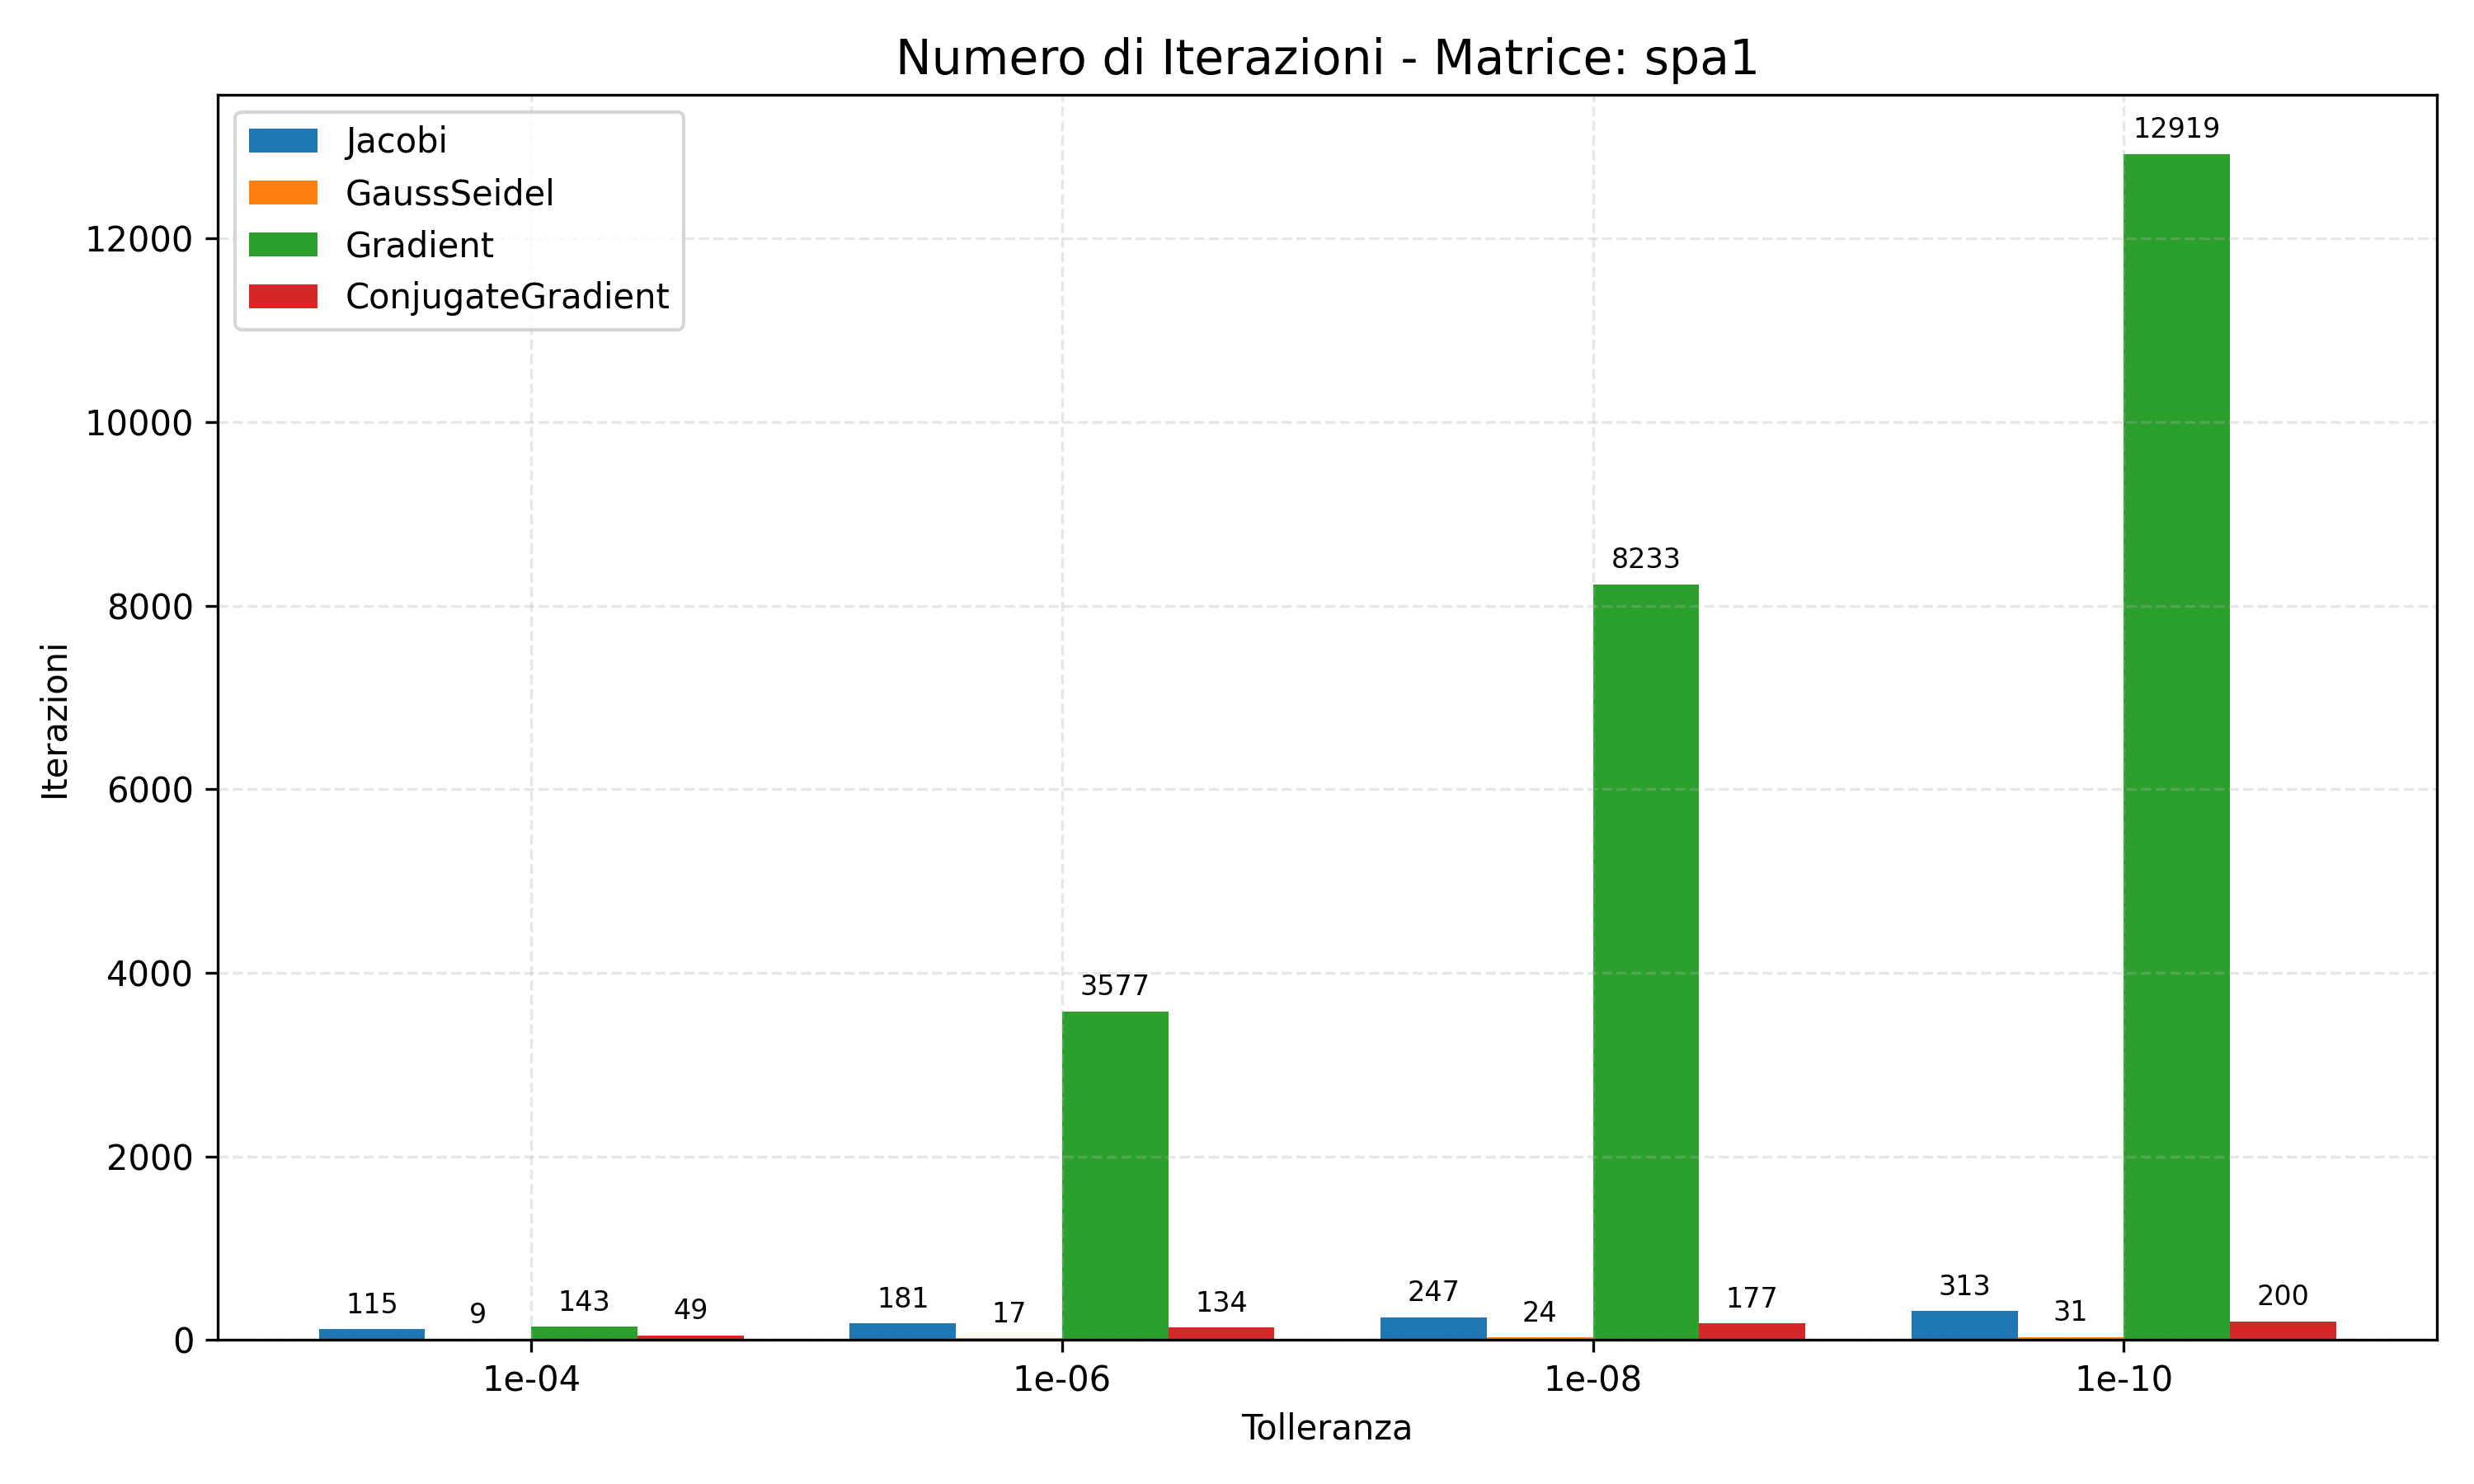
\includegraphics[width=0.9\textwidth]{plots/spa1_iterations.png}
    \caption{Numero di iterazioni per spa1}
\end{figure}

Dal grafico si nota che il metodo del \textbf{Gradiente} impiega un numero di iterazioni nettamente superiore rispetto agli altri man mano che la tolleranza diminuisce. Questo comportamento è dovuto a un elevato numero di condizionamento della matrice. 

Al contrario, il metodo di \textbf{Gau\ss{}-Seidel} risulta essere il più efficiente in assoluto, risolvendo il sistema con il minor numero di passi. Il \textbf{Gradiente Coniugato}, pur non essendo il minimo assoluto, mantiene prestazioni eccellenti superando di gran lunga il Gradiente standard, grazie allo sfruttamento delle direzioni $A$-ortogonali. Infine, il metodo di \textbf{Jacobi} si assesta su valori intermedi: pur necessitando di più iterazioni rispetto a Gau\ss{}-Seidel e al Gradiente Coniugato, risulta comunque molto più rapido a convergere rispetto al Gradiente.

\subsection{Analisi dei Tempi}
\begin{figure}[H]
    \centering
    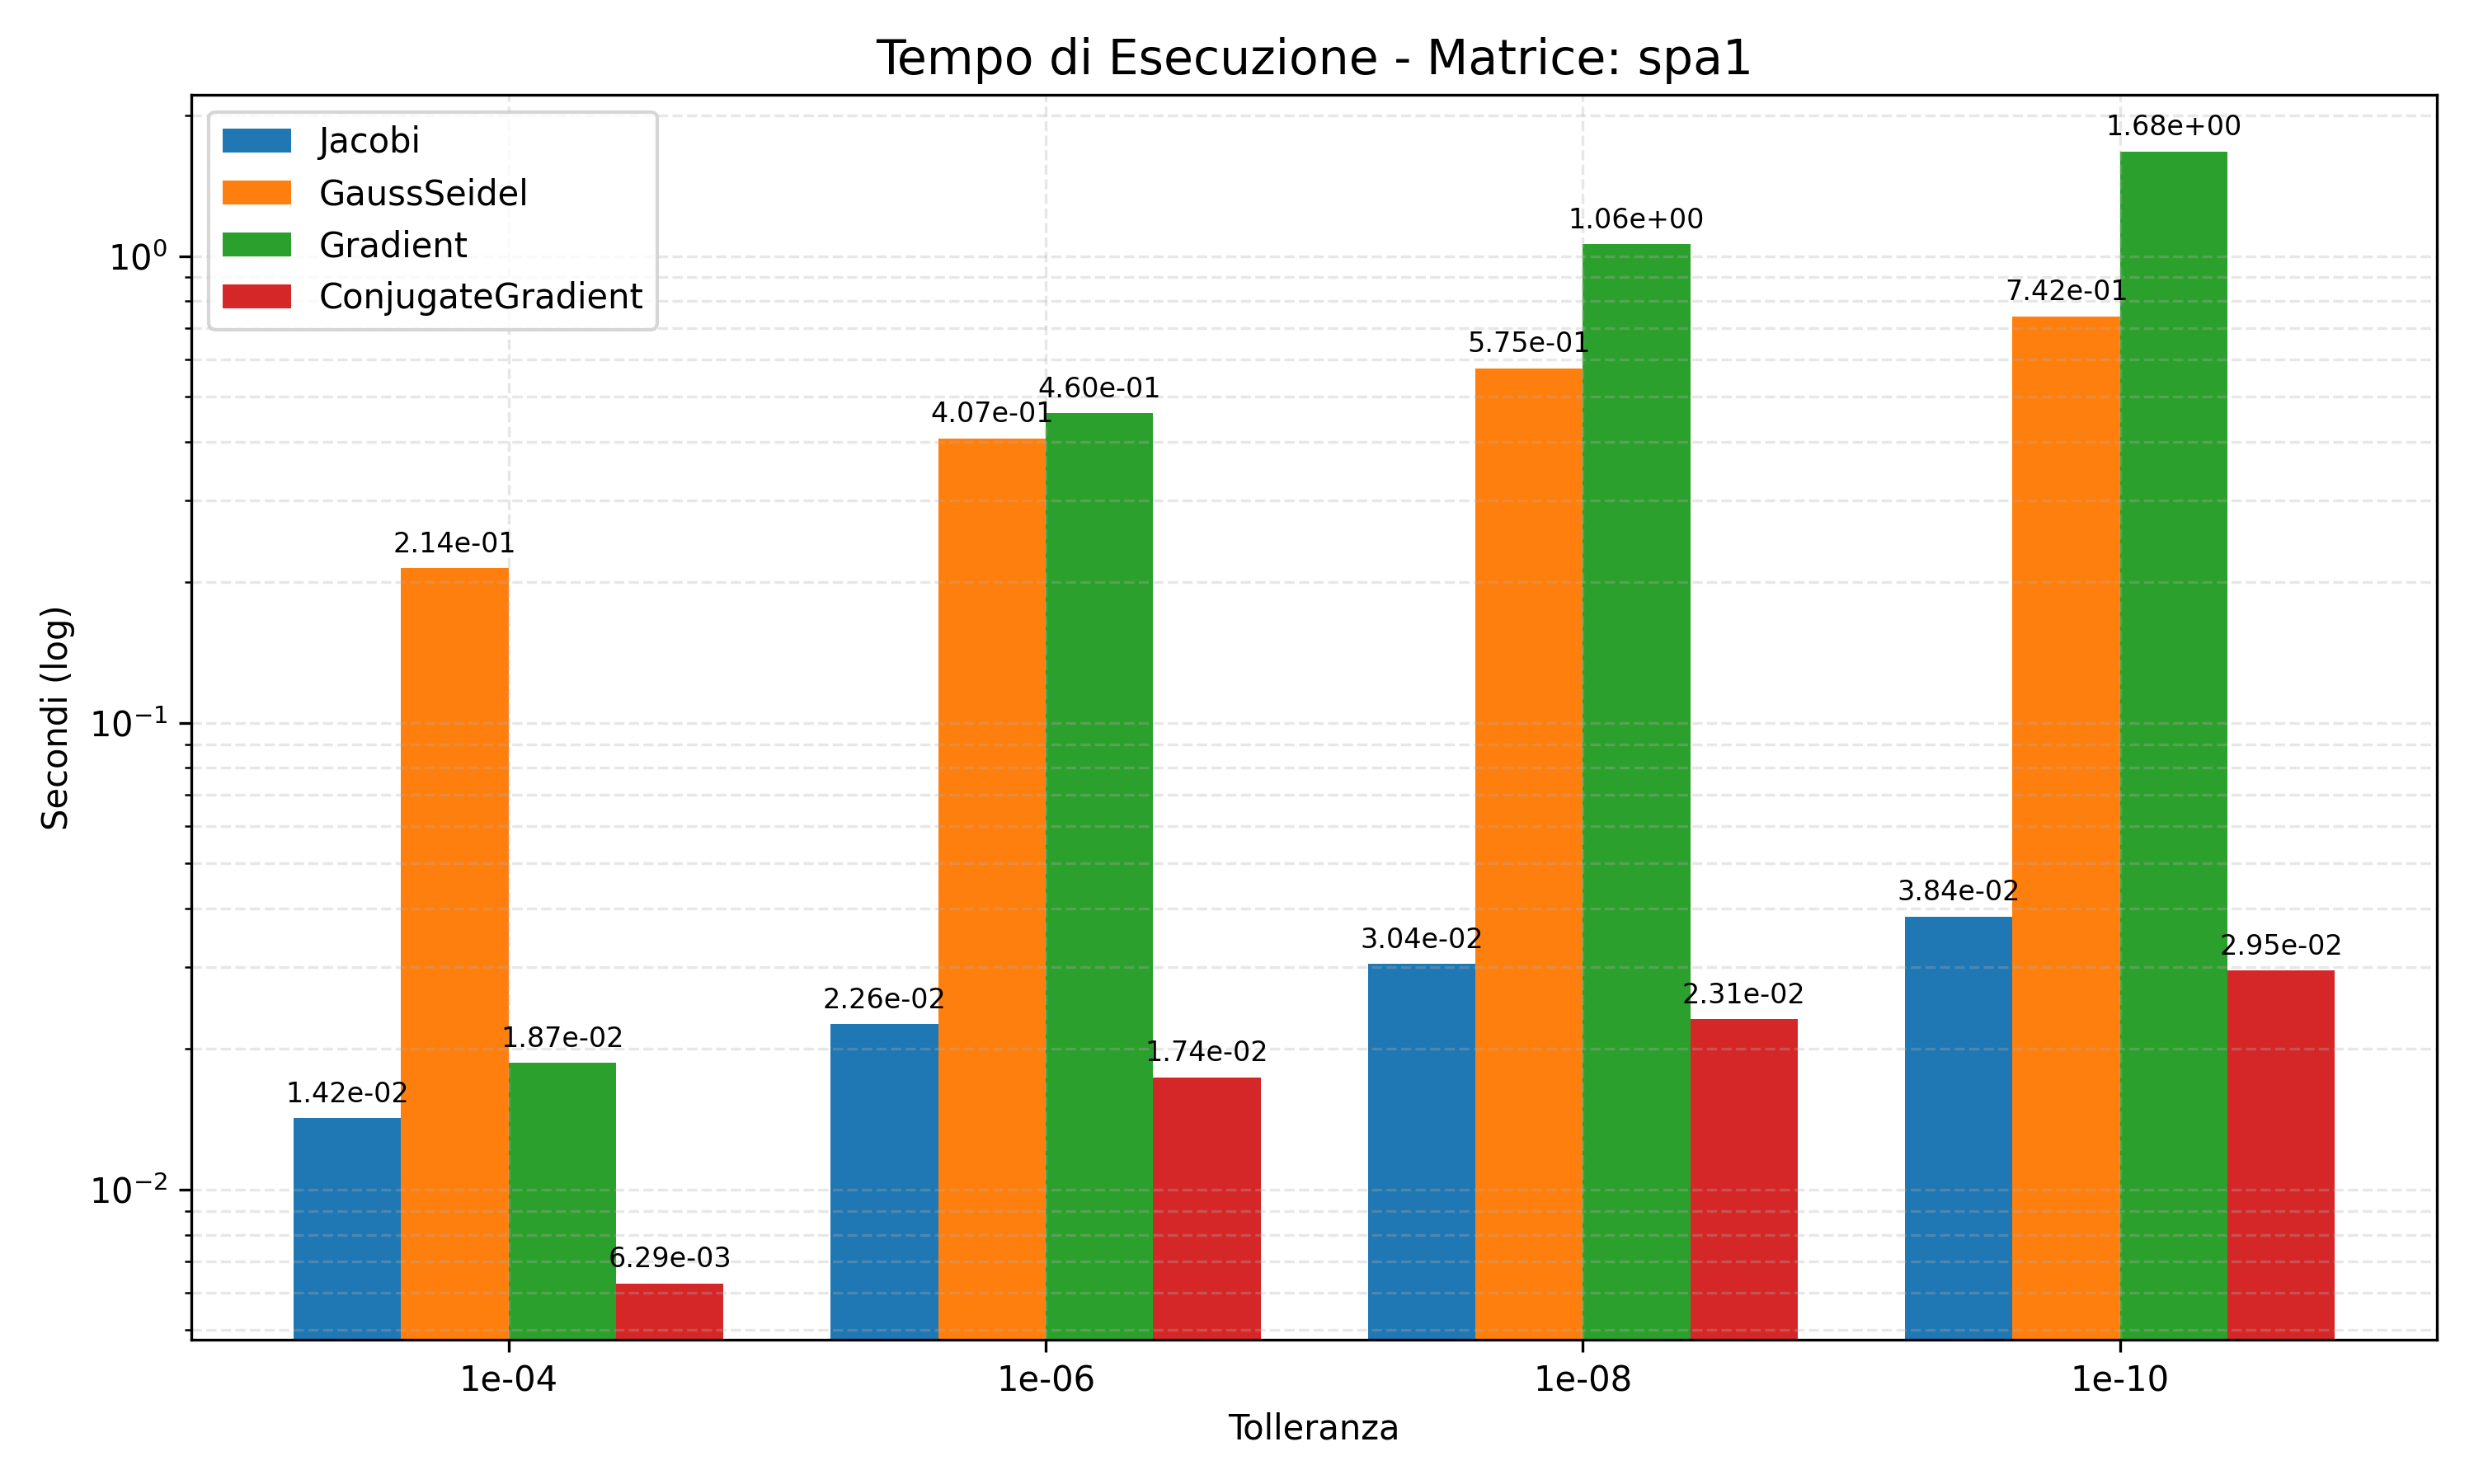
\includegraphics[width=0.9\textwidth]{plots/spa1_time.png}
    \caption{Tempo di esecuzione per spa1}
\end{figure}

Analizzando invece i tempi di esecuzione, il \textbf{Gradiente Coniugato} risulta l'algoritmo più veloce, seguito dal metodo di \textbf{Jacobi}, che mostra prestazioni competitive. Al contrario, sebbene \textbf{Gau\ss{}-Seidel} richiedesse il minor numero di iterazioni, il suo tempo di esecuzione è notevolmente più alto degli altri (ad eccezione del \textbf{Gradiente} che risulta il più lento del gruppo). Questa discrepanza tra basso numero di iterazioni e alto tempo di calcolo è da imputare all'implementazione, infatti nel nostro algoritmo a ogni iterazione di Gau\ss{}-Seidel viene richiamata una funzione custom (\texttt{forward\_substitution\_csr}) per la risoluzione del sistema triangolare inferiore. Questo causa un notevole rallentamento rispetto alle funzioni offerte da librerie come SciPy, come mostrato nella sezione successiva.

\subsection{Confronto Implementazioni Gau\ss{}-Seidel}
\begin{figure}[H]
    \centering
    % Lasciato lo spazio per i due grafici affiancati
    \begin{minipage}{0.48\textwidth}
        \centering
        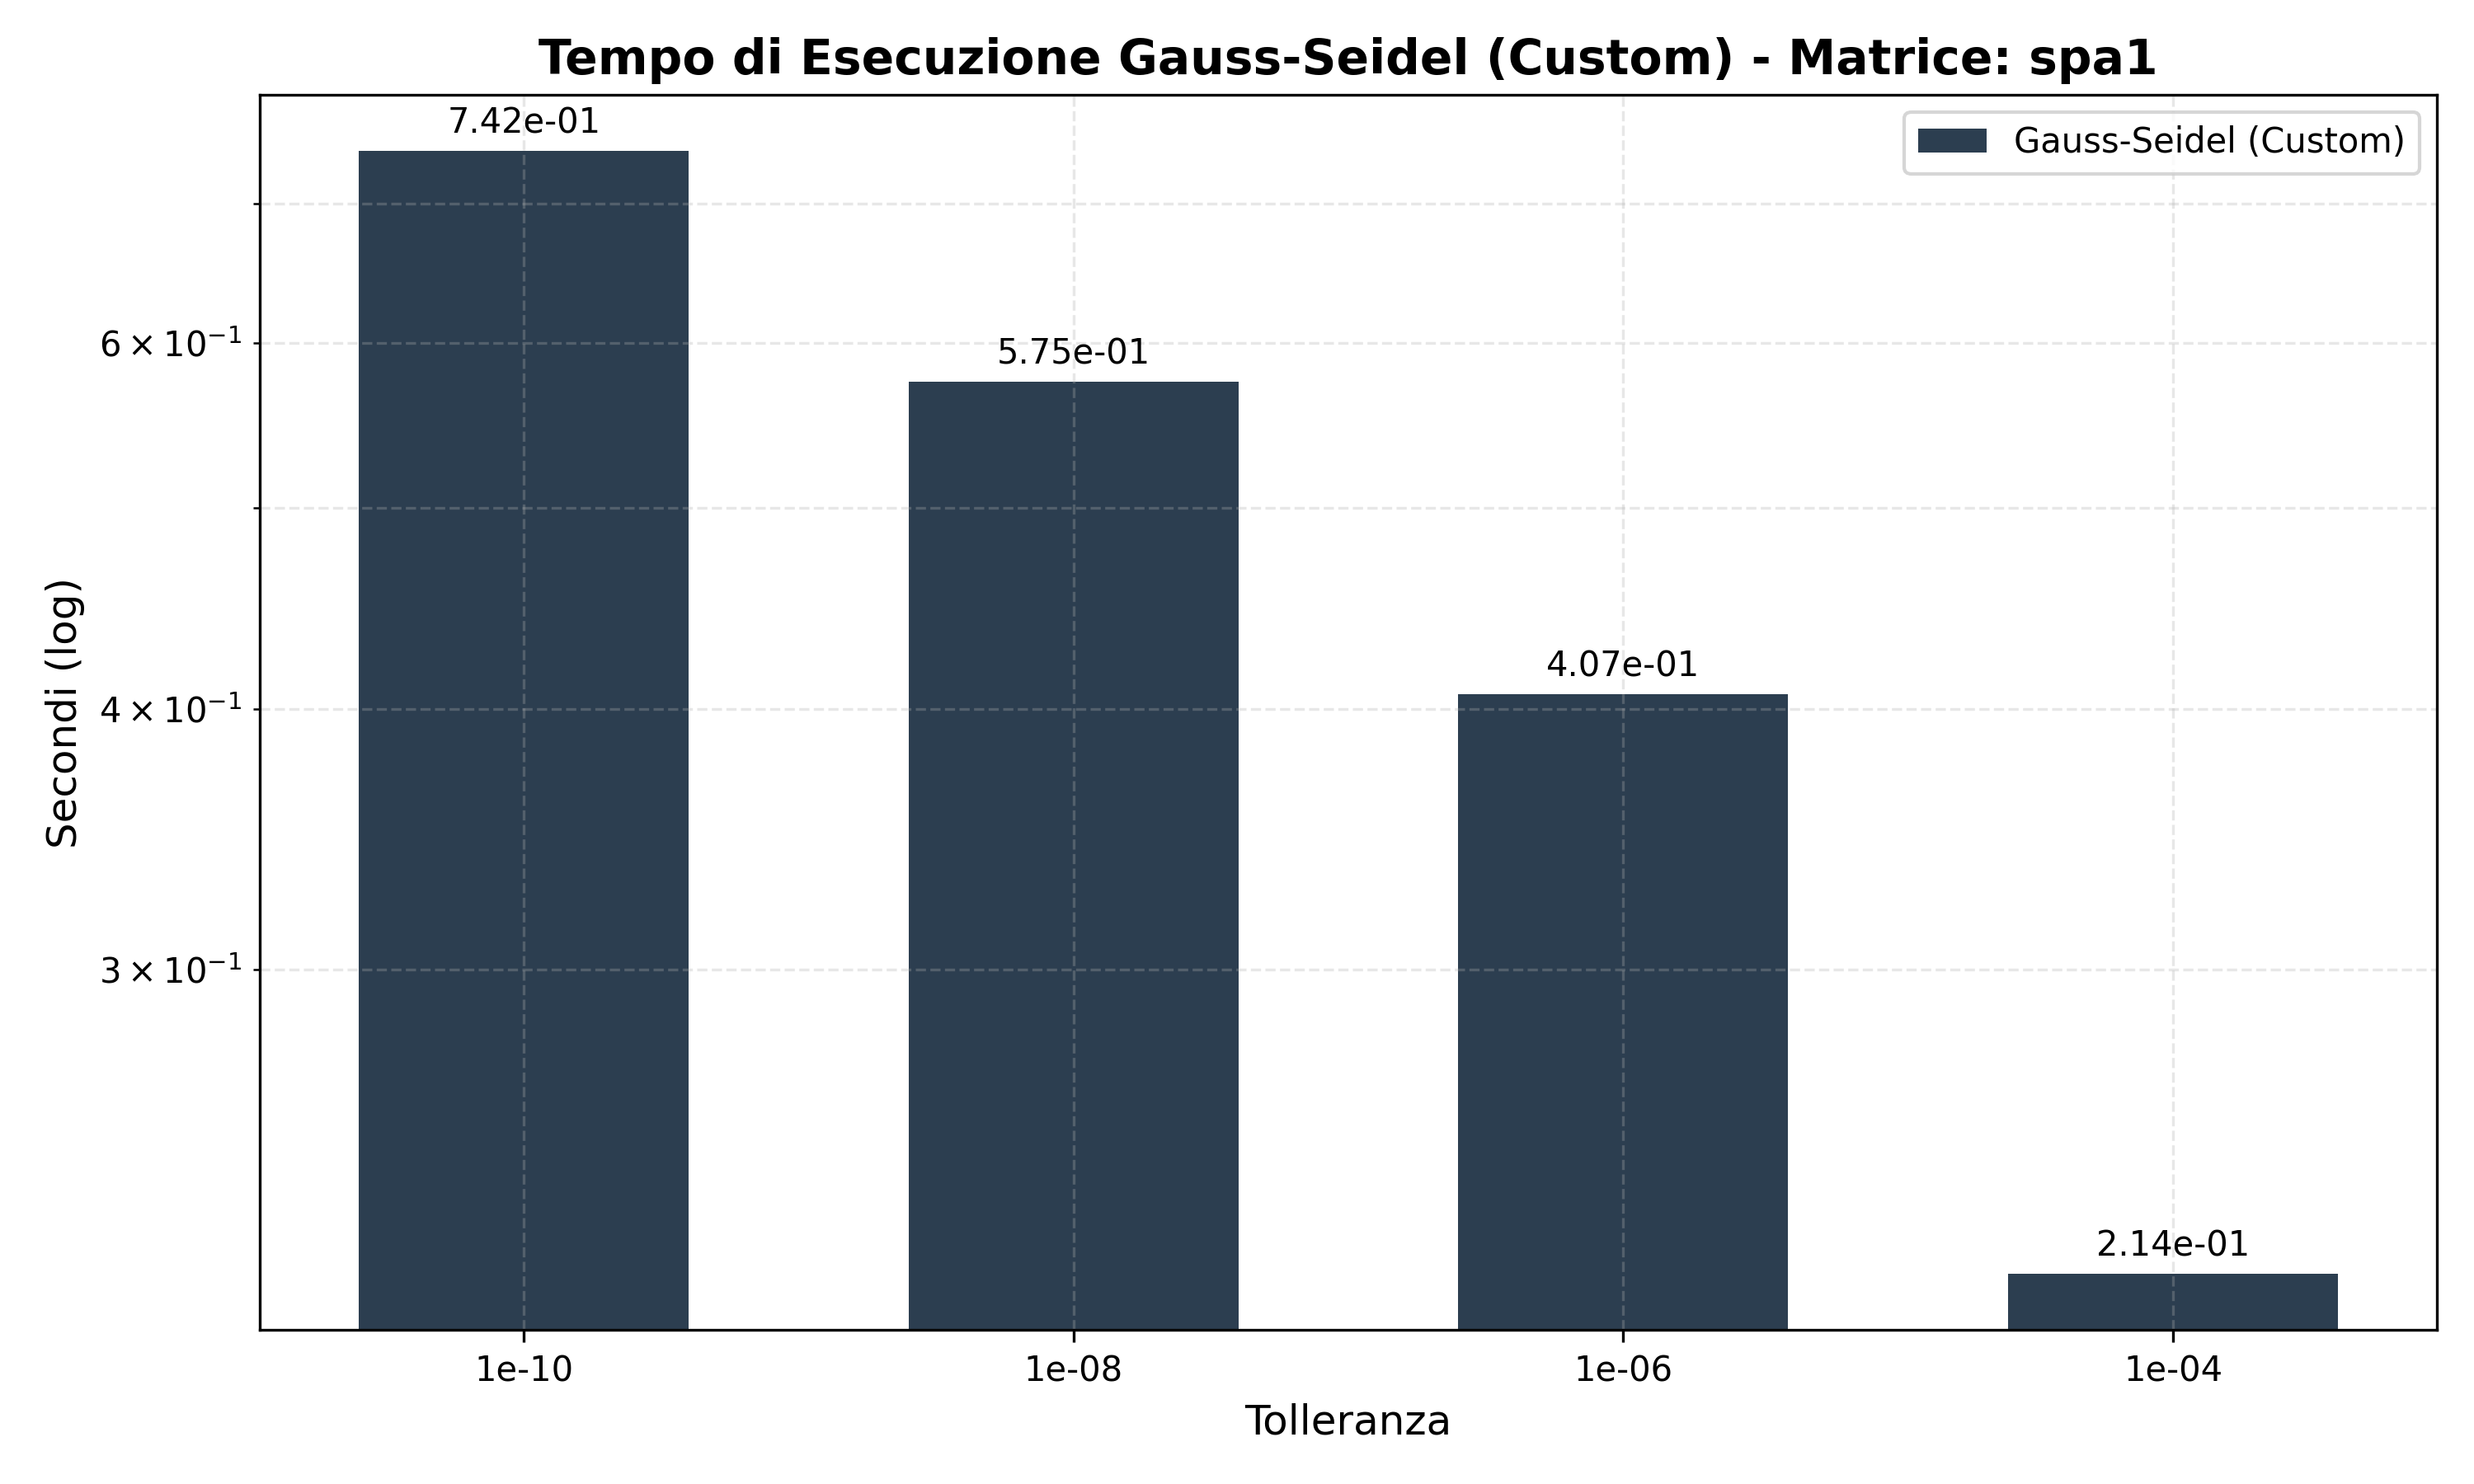
\includegraphics[width=\textwidth]{plots/gs_custom_spa1.png} % Da sostituire
        \caption{GS Custom (Forward Sub)}
    \end{minipage}\hfill
    \begin{minipage}{0.48\textwidth}
        \centering
        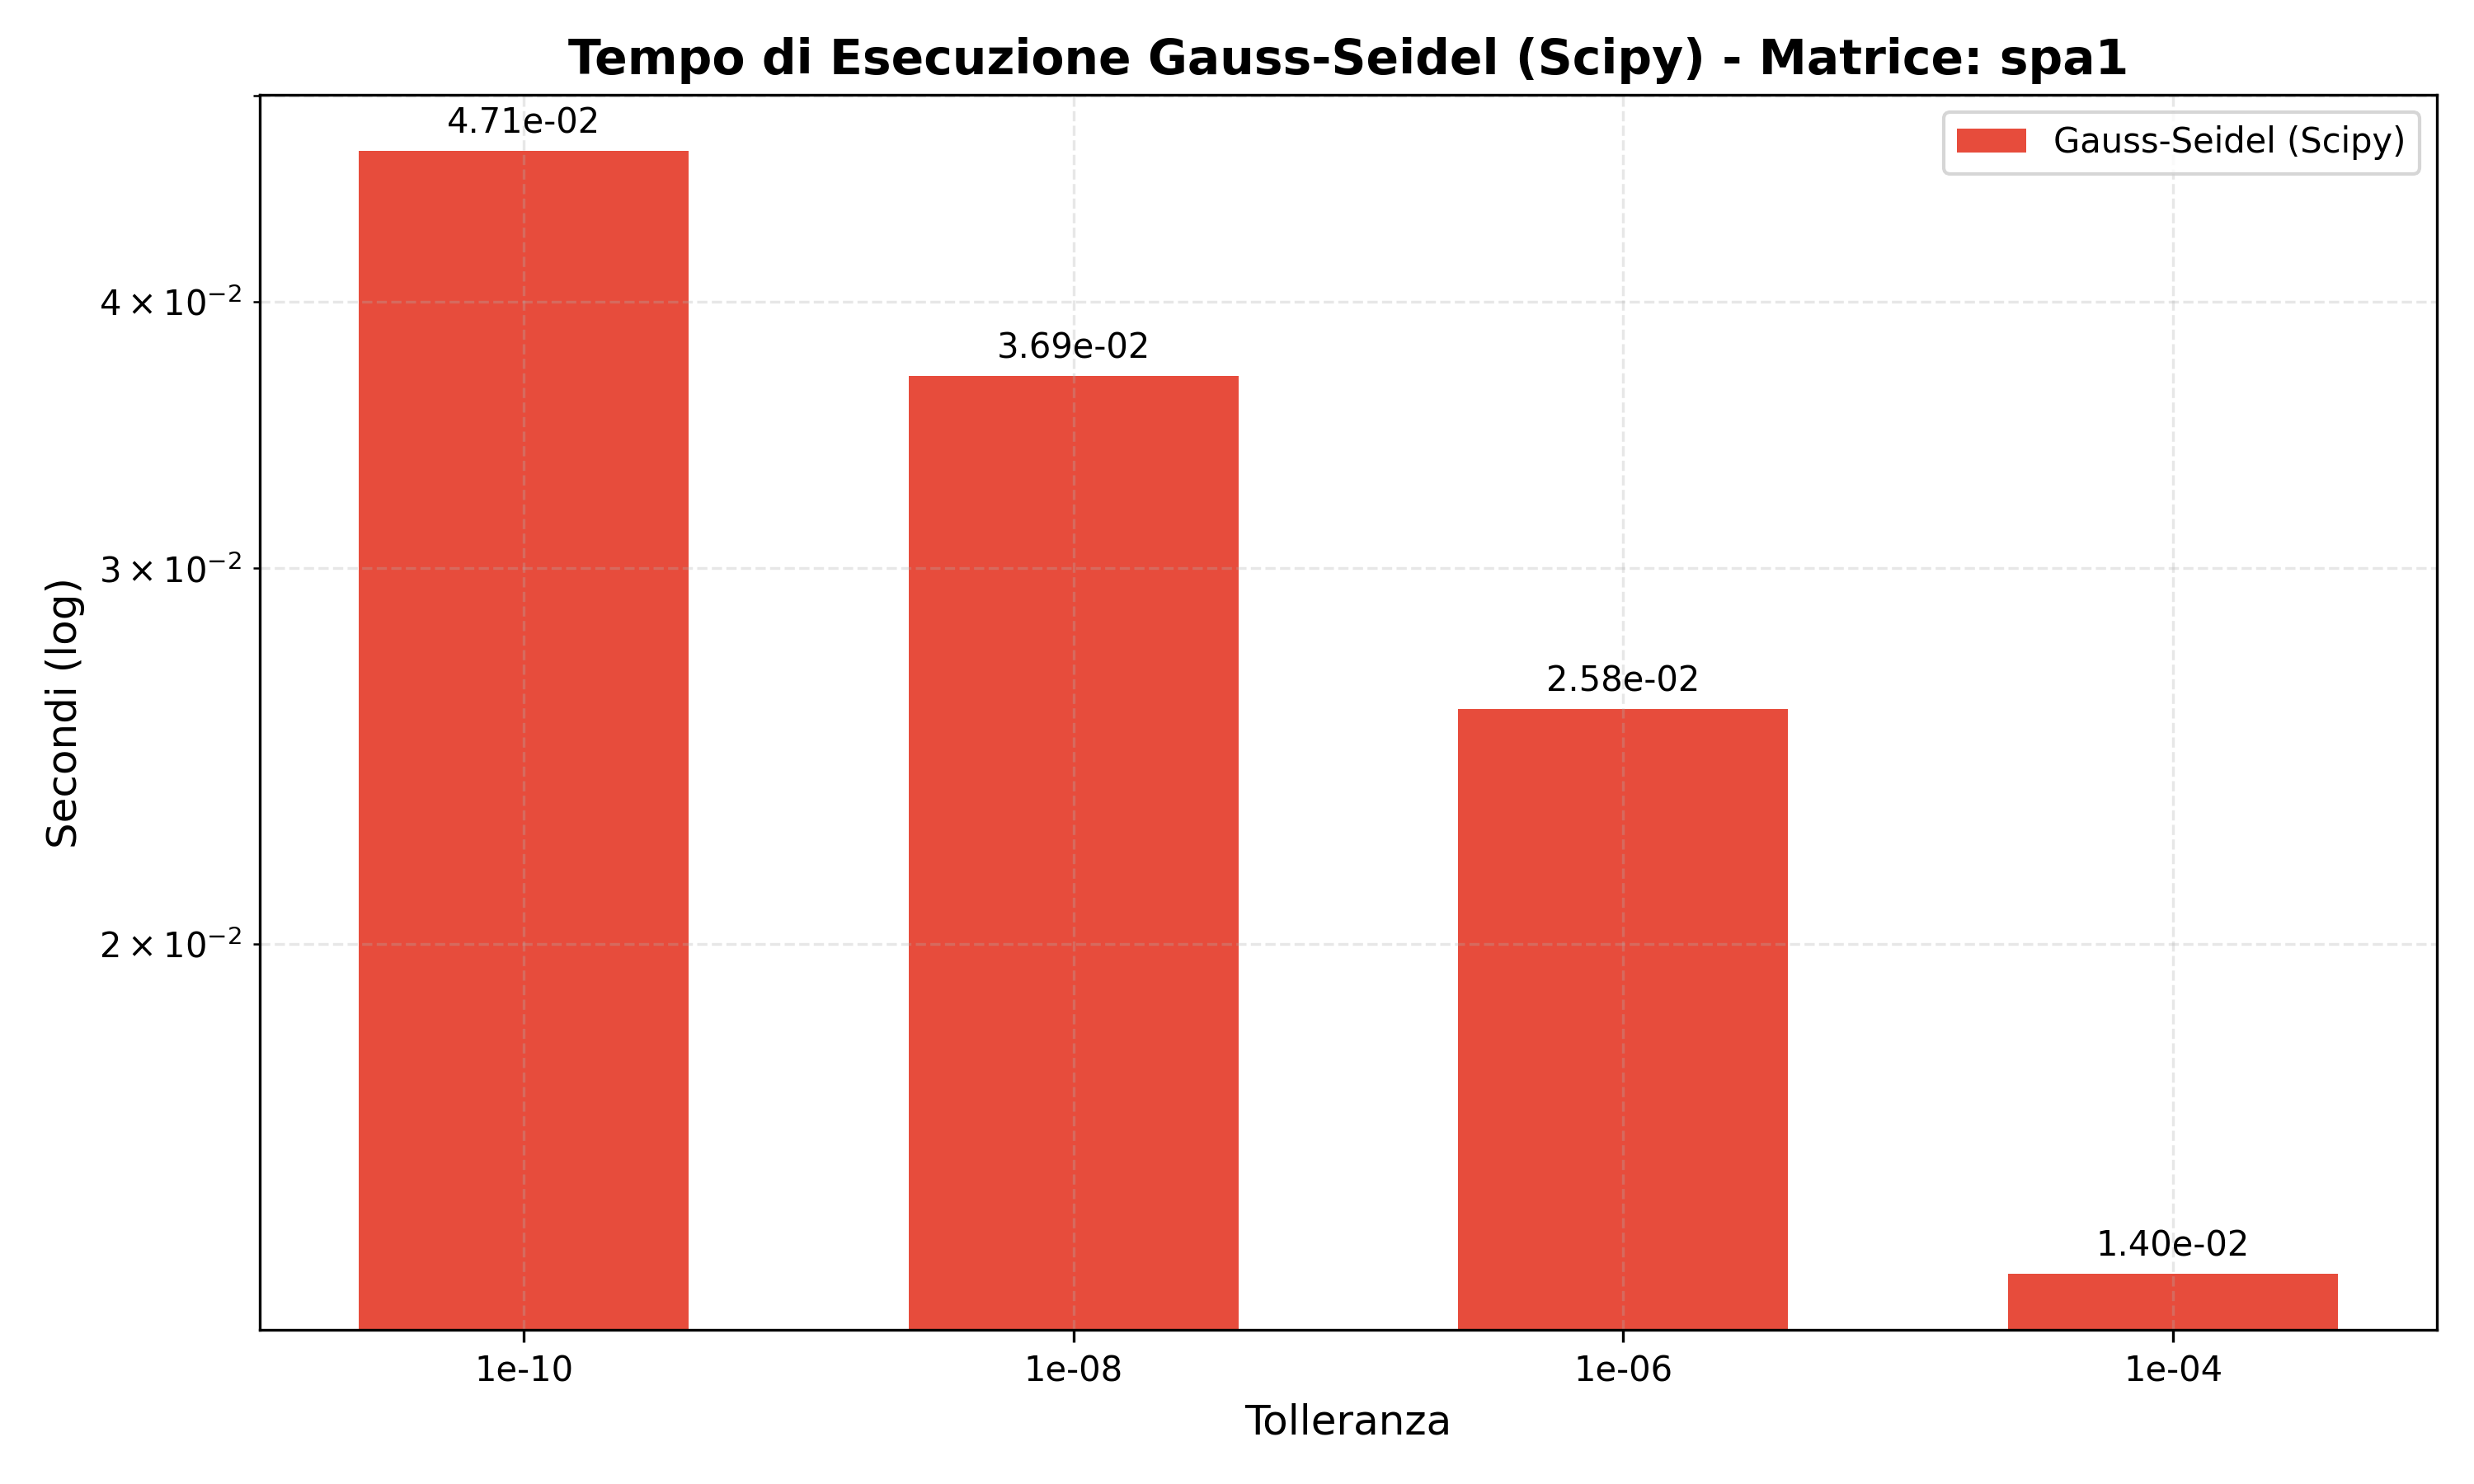
\includegraphics[width=\textwidth]{plots/gs_scipy_spa1.png} % Da sostituire
        \caption{GS SciPy (spsolve\_triangular)}
    \end{minipage}
\end{figure}

Come discusso nel capitolo precedente, è stato condotto un confronto diretto tra l'implementazione custom di sostituzione in avanti e la funzione ottimizzata in C offerta da SciPy (\texttt{spsolve\_triangular}). I grafici illustrano il tempo totale di esecuzione dell'algoritmo, e non quello della singola iterazione. A parità di iterazioni e di errore relativo, l'implementazione manuale mostra una notevole lentezza del loop nativo di Python rispetto alle funzioni pre-compilate della libreria.

\subsection{Analisi dell'Errore Relativo}
\begin{figure}[H]
    \centering
    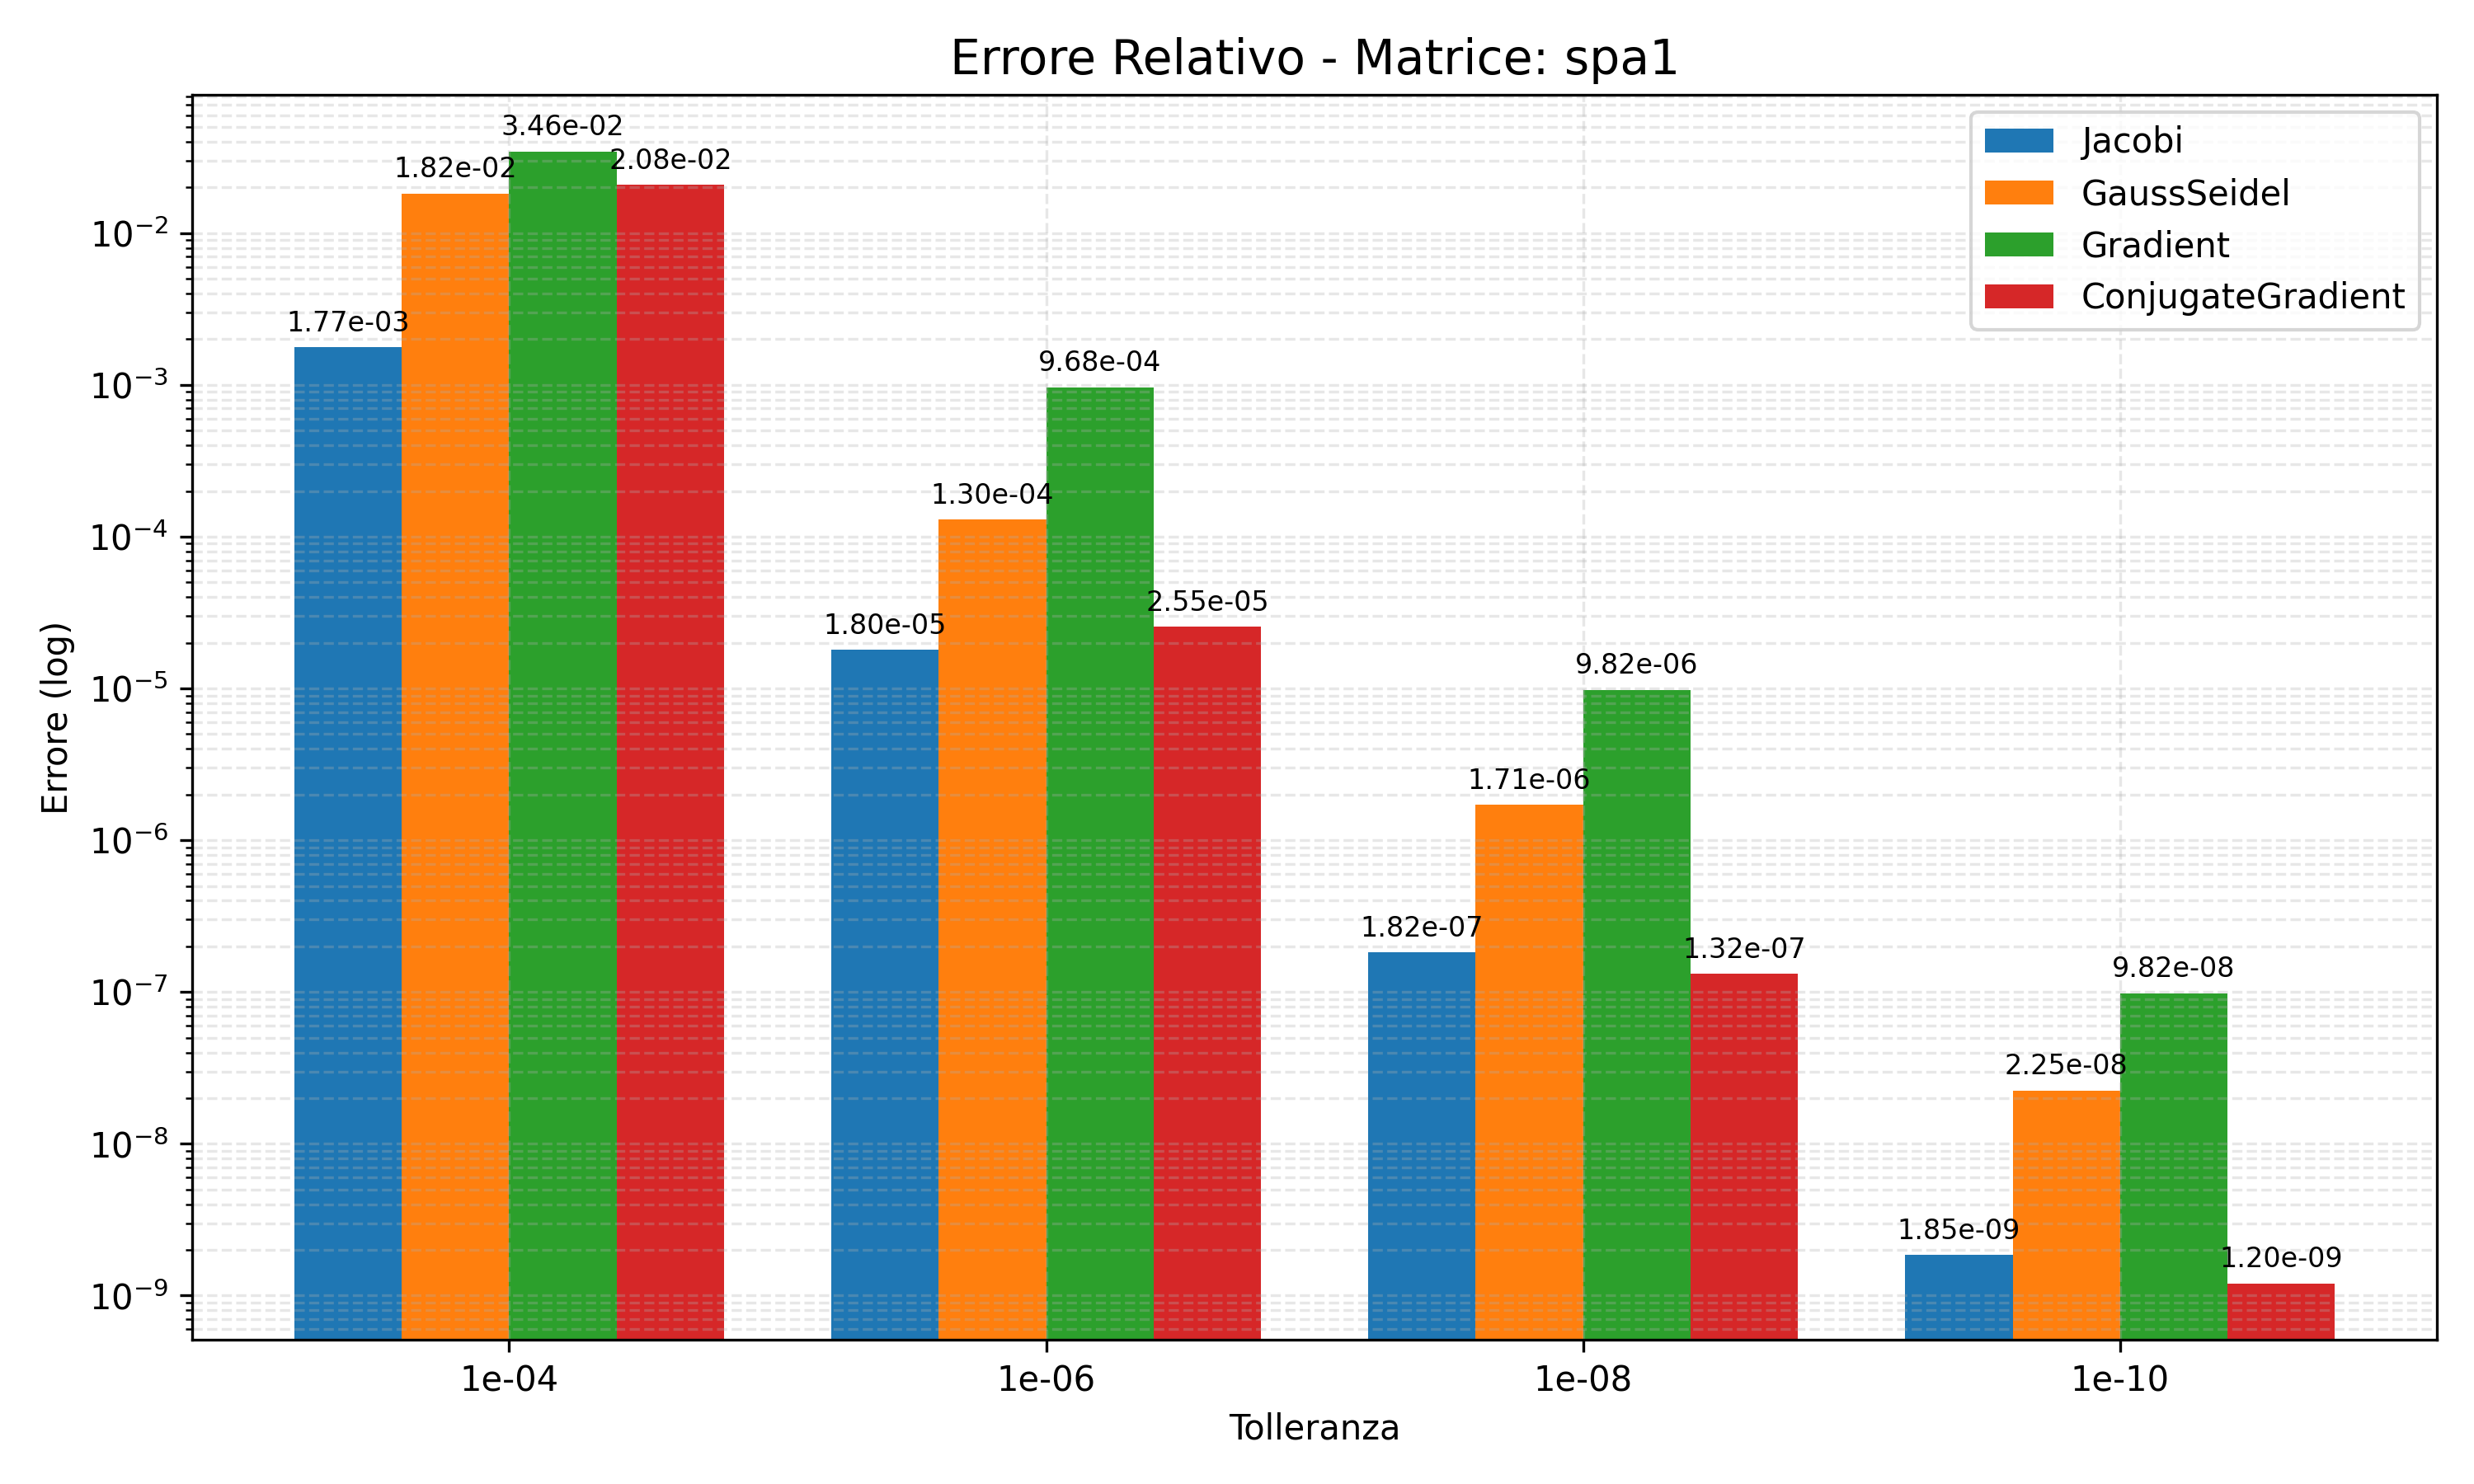
\includegraphics[width=0.9\textwidth]{plots/spa1_error.png}
    \caption{Errore relativo per spa1}
\end{figure}

Si nota che tutti i metodi riescono a soddisfare le tolleranze richieste decrescendo in modo costante. Il metodo del \textbf{Gradiente Coniugato} e quello di \textbf{Jacobi} raggiungono costantemente i valori di errore più bassi, dimostrando un'eccellente precisione finale per ogni soglia di tolleranza. Il metodo di \textbf{Gau\ss{}-Seidel} si posiziona su valori leggermente superiori, mentre il metodo del \textbf{Gradiente} standard registra l'errore relativo più alto a convergenza, confermando le difficoltà numeriche legate al malcondizionamento della matrice.

\section{Matrice: spa2}
\subsection{Analisi della Matrice}
In questa sottosezione viene presentata l'analisi morfologica della matrice \texttt{spa2}. La tabella \ref{tab:analisi_spa2} ne riassume le caratteristiche strutturali, mentre la figura \ref{fig:heatmap_spa2} ne mostra la distribuzione dei valori tramite heatmap.

\begin{figure}[H]
    \centering
    % Prima colonna per la tabella
    \begin{minipage}[c]{0.48\textwidth}
        \centering
        \begin{tabular}{lr}
            \toprule
            \multicolumn{2}{l}{\textbf{Matrice spa2}} \\
            \midrule
            \textbf{Rows} & 3000 \\
            \textbf{Cols} & 3000 \\
            \textbf{Area} & 9000000 \\
            \textbf{Density (\%)} & 18.148 \\
            \textbf{Mean} & 3.3427 \\
            \textbf{Std Dev} & 74.89 \\
            \textbf{Condition Number} & 1412.0 \\
            \bottomrule
        \end{tabular}
        \captionof{table}{Tabella spa2}
        \label{tab:analisi_spa2}
    \end{minipage}\hfill
    \begin{minipage}[c]{0.48\textwidth}
        \centering
        \includegraphics[width=\linewidth]{plots/spa2_heatmap.png}
        \captionof{figure}{Heatmap spa2}
        \label{fig:heatmap_spa2}
    \end{minipage}
\end{figure}

Nonostante il numero di condizionamento di spa2 (1412.0) sia più basso rispetto a spa1 (2048.2), i tempi di esecuzione risultano comunque più alti. Questo è dovuto alle dimensioni notevolmente maggiori del sistema, che aumentano il costo di ogni singola iterazione e compensano ampiamente il vantaggio dato dal condizionamento migliore.

\subsection{Risultati Numerici}
La seguente tabella riassume i risultati ottenuti per i quattro algoritmi al variare della tolleranza richiesta per la matrice \texttt{spa2}.

\begin{table}[H]
    \centering
    \begin{tabular}{|c|c|c|c|c|}
        \hline
        \textbf{Tol} & \textbf{Metodo} & \textbf{Numero iterazioni} & \textbf{Tempo (s)} & \textbf{Errore relativo} \\
        \hline
        $10^{-4}$ & Jacobi & 36 & 0.0498 & $1.77 \cdot 10^{-3}$ \\
                  & Gauss-Seidel & 5 & 1.0700 & $2.60 \cdot 10^{-3}$ \\
                  & Gradient & 161 & 0.1989 & $1.81 \cdot 10^{-2}$ \\
                  & Conjugate Gradient & 42 & 0.0543 & $9.82 \cdot 10^{-3}$ \\
        \hline
        $10^{-6}$ & Jacobi & 57 & 0.0670 & $1.67 \cdot 10^{-5}$ \\
                  & Gauss-Seidel & 8 & 1.7256 & $5.14 \cdot 10^{-5}$ \\
                  & Gradient & 1949 & 2.3218 & $6.69 \cdot 10^{-4}$ \\
                  & Conjugate Gradient & 122 & 0.1482 & $1.20 \cdot 10^{-4}$ \\
        \hline
        $10^{-8}$ & Jacobi & 78 & 0.0873 & $1.57 \cdot 10^{-7}$ \\
                  & Gauss-Seidel & 12 & 2.5786 & $2.79 \cdot 10^{-7}$ \\
                  & Gradient & 5087 & 6.0056 & $6.87 \cdot 10^{-6}$ \\
                  & Conjugate Gradient & 196 & 0.2238 & $5.59 \cdot 10^{-7}$ \\
        \hline
        $10^{-10}$ & Jacobi & 99 & 0.1071 & $1.48 \cdot 10^{-9}$ \\
                  & Gauss-Seidel & 15 & 3.2689 & $5.57 \cdot 10^{-9}$ \\
                  & Gradient & 8285 & 9.6796 & $6.94 \cdot 10^{-8}$ \\
                  & Conjugate Gradient & 240 & 0.2841 & $5.32 \cdot 10^{-9}$ \\
        \hline
    \end{tabular}
    \caption{Risultati numerici per spa2}
\end{table}

\subsection{Analisi delle Iterazioni}
\begin{figure}[H]
    \centering
    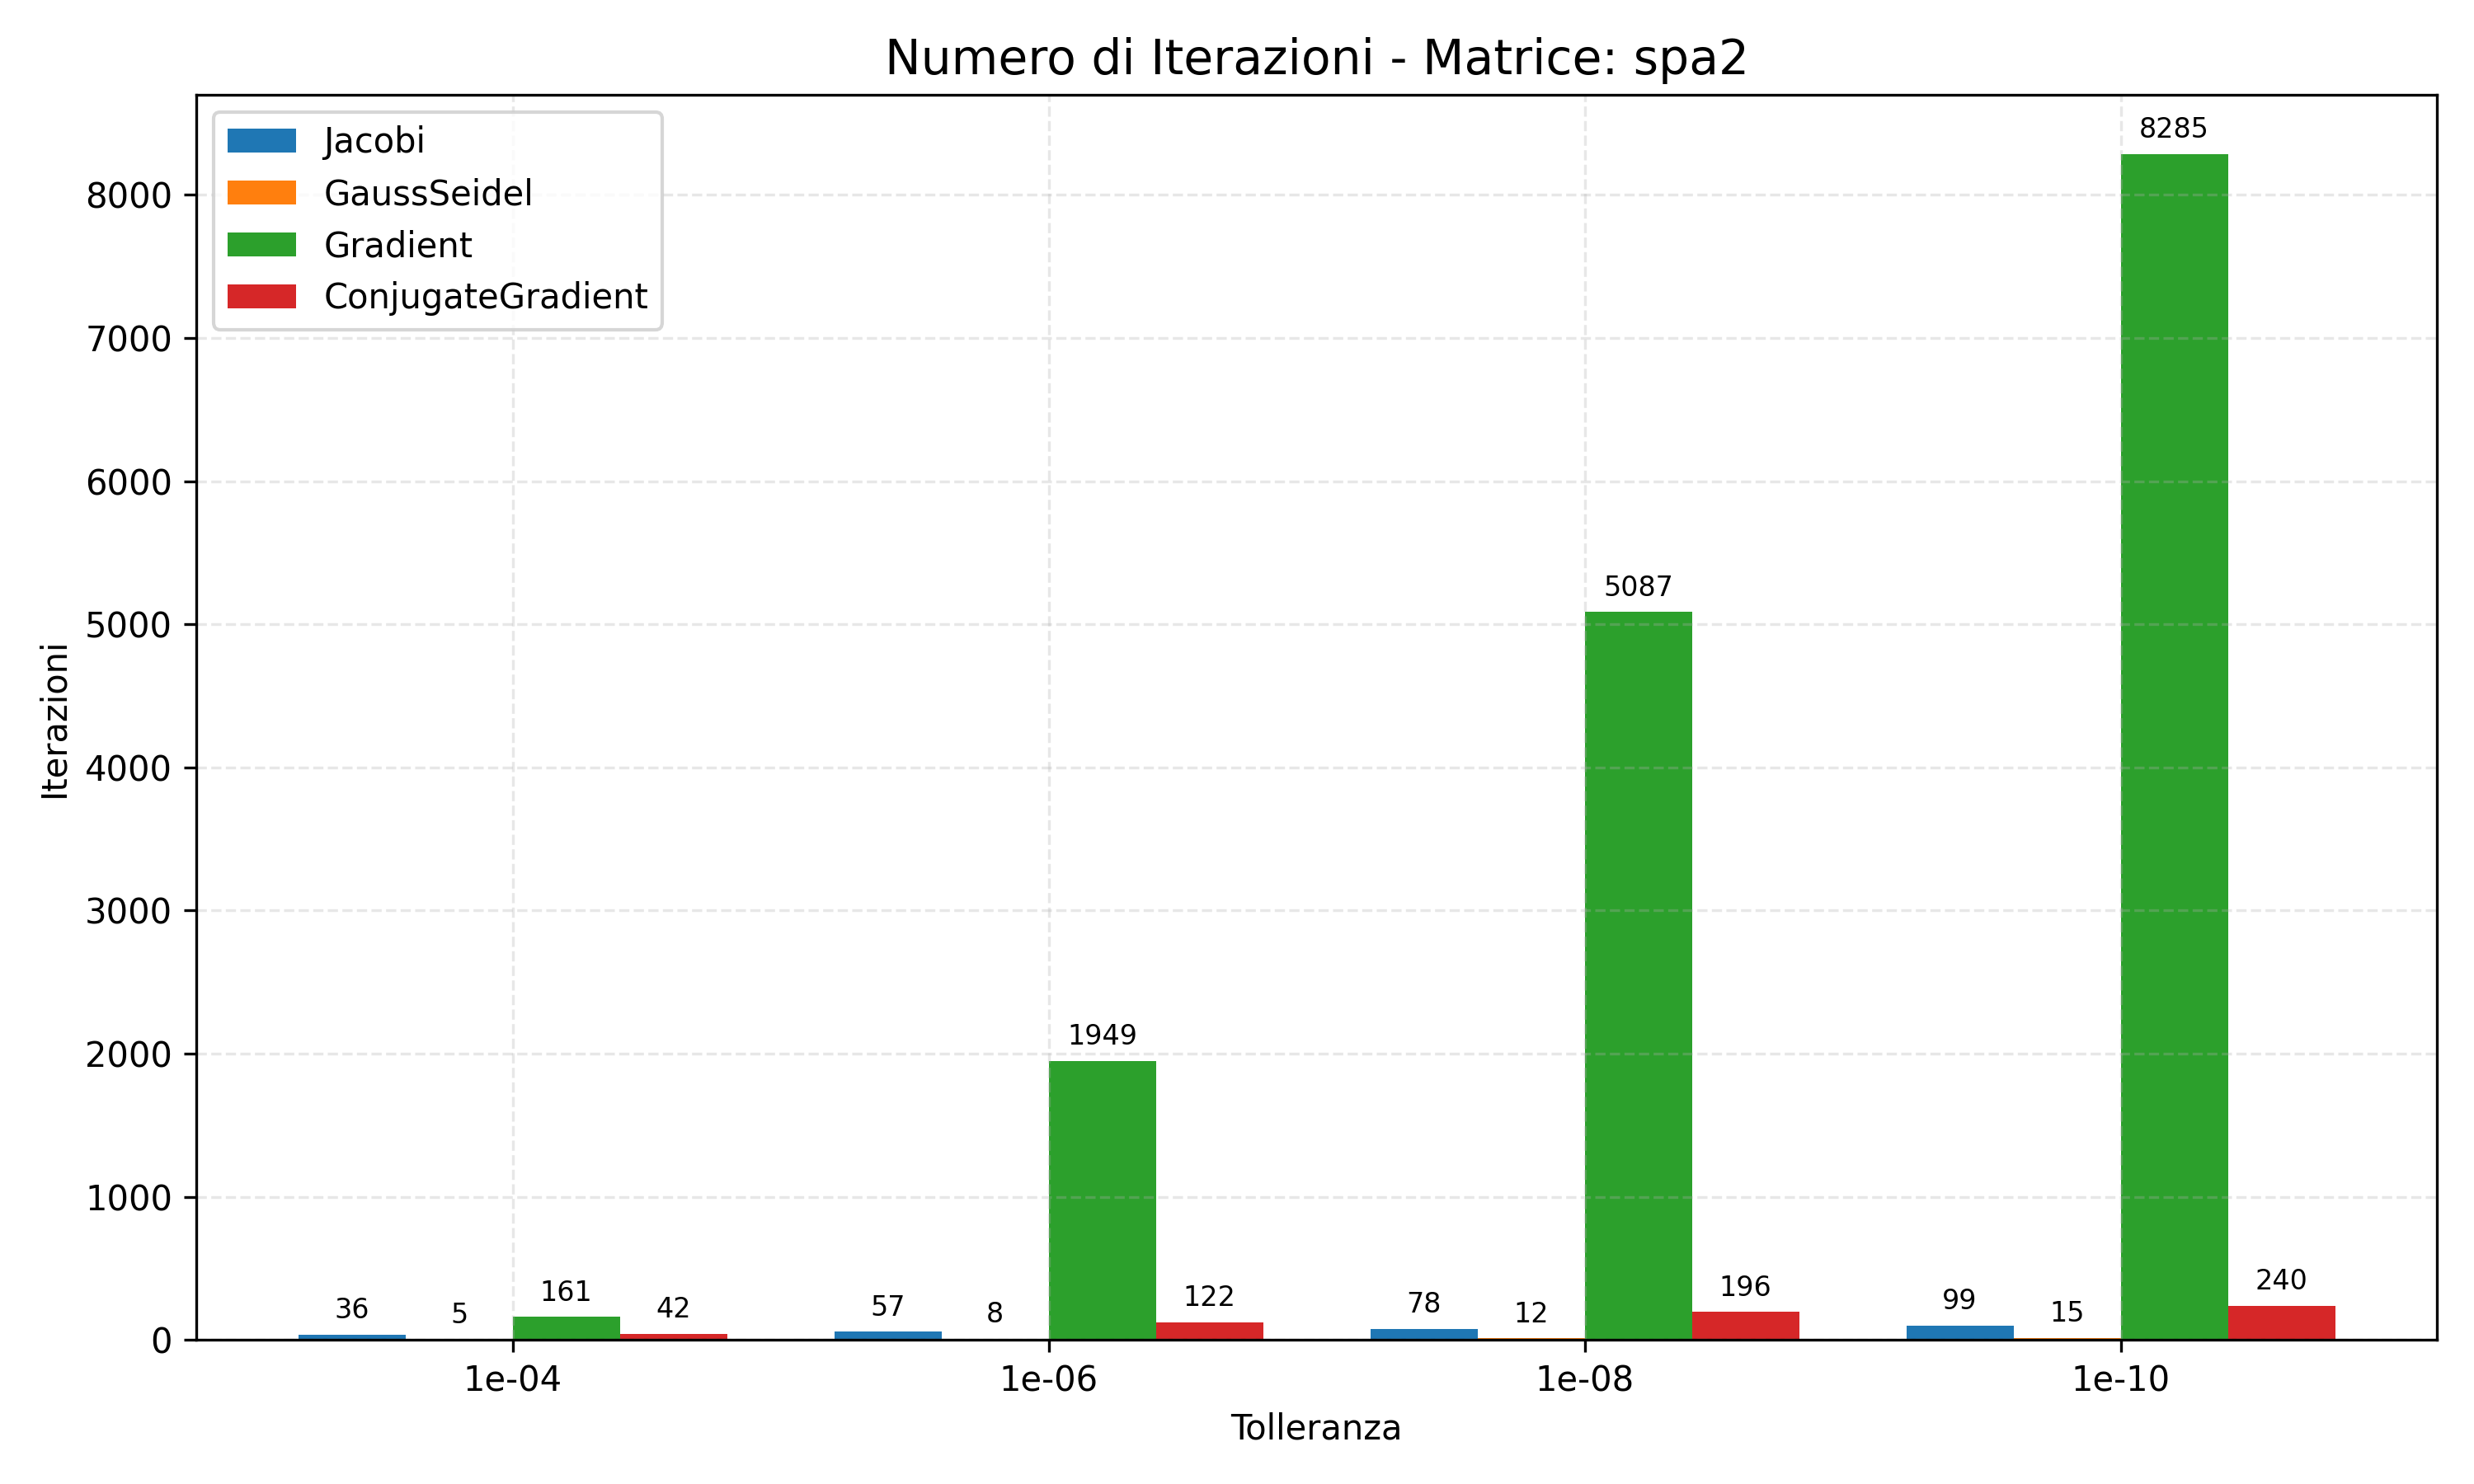
\includegraphics[width=0.9\textwidth]{plots/spa2_iterations.png}
    \caption{Numero di iterazioni per spa2}
\end{figure}

Si osserva un andamento qualitativamente simile a quello riscontrato per \texttt{spa1}. Il metodo del \textbf{Gradiente} mostra una rapida crescita del numero di iterazioni al diminuire della tolleranza, mentre il \textbf{Gau\ss{}-Seidel} risulta di gran lunga il più efficiente, convergendo nel minor numero di iterazioni. A differenza del caso precedente, per la matrice \texttt{spa2} il metodo di \textbf{Jacobi} risulta più performante del \textbf{Gradiente Coniugato}, richiedendo un numero di iterazioni costantemente inferiore per ogni livello di tolleranza. Entrambi si mantengono comunque su valori ottimali, confermando un netto vantaggio rispetto alle scarse prestazioni del Gradiente standard.

\subsection{Analisi dei Tempi}
\begin{figure}[H]
    \centering
    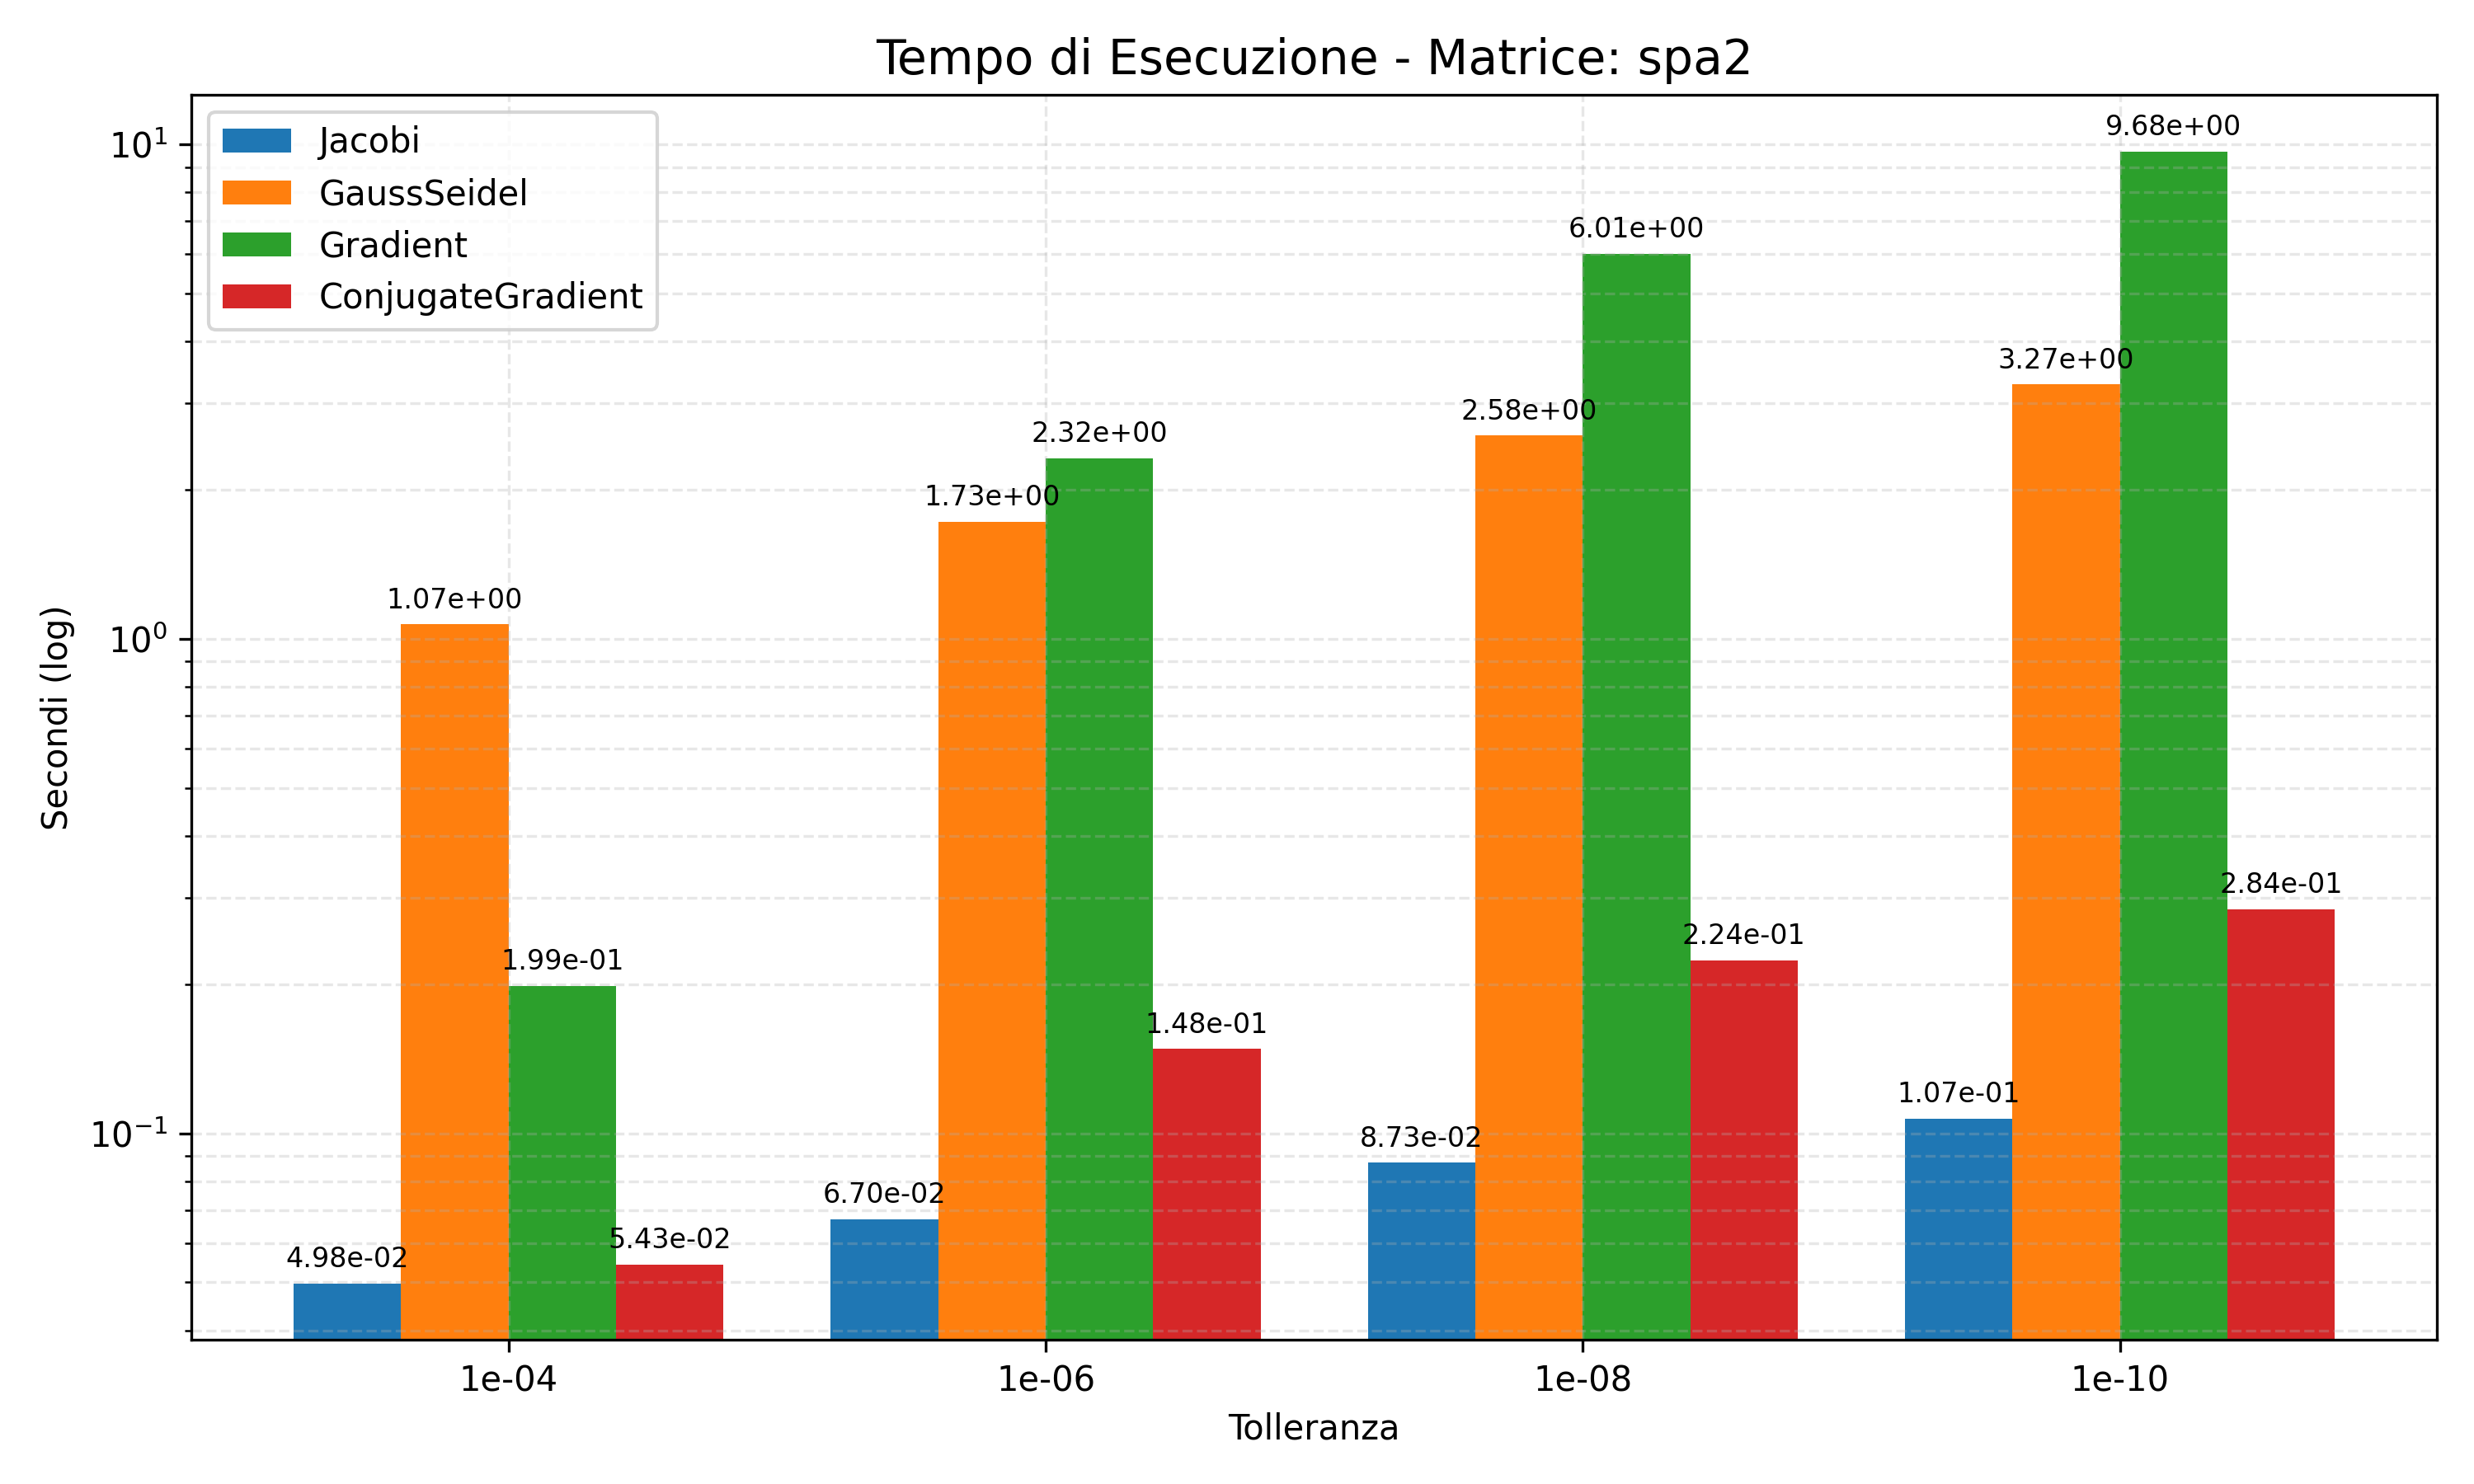
\includegraphics[width=0.9\textwidth]{plots/spa2_time.png}
    \caption{Tempo di esecuzione per spa2}
\end{figure}

Analizzando invece i tempi di esecuzione, il \textbf{Gradiente Coniugato} e il metodo di \textbf{Jacobi} si confermano gli algoritmi più veloci, mostrando entrambi prestazioni eccellenti. Al contrario, sebbene \textbf{Gau\ss{}-Seidel} richieda il minor numero di iterazioni in assoluto, il suo tempo di esecuzione è notevolmente più alto degli altri, venendo superato solo dal \textbf{Gradiente}. Come già osservato in precedenza, questa discrepanza per Gau\ss{}-Seidel è da imputare all'utilizzo della funzione custom per la risoluzione del sistema triangolare inferiore.

\subsection{Confronto Implementazioni Gauß-Seidel}
\begin{figure}[H]
    \centering
    \begin{minipage}{0.48\textwidth}
        \centering
        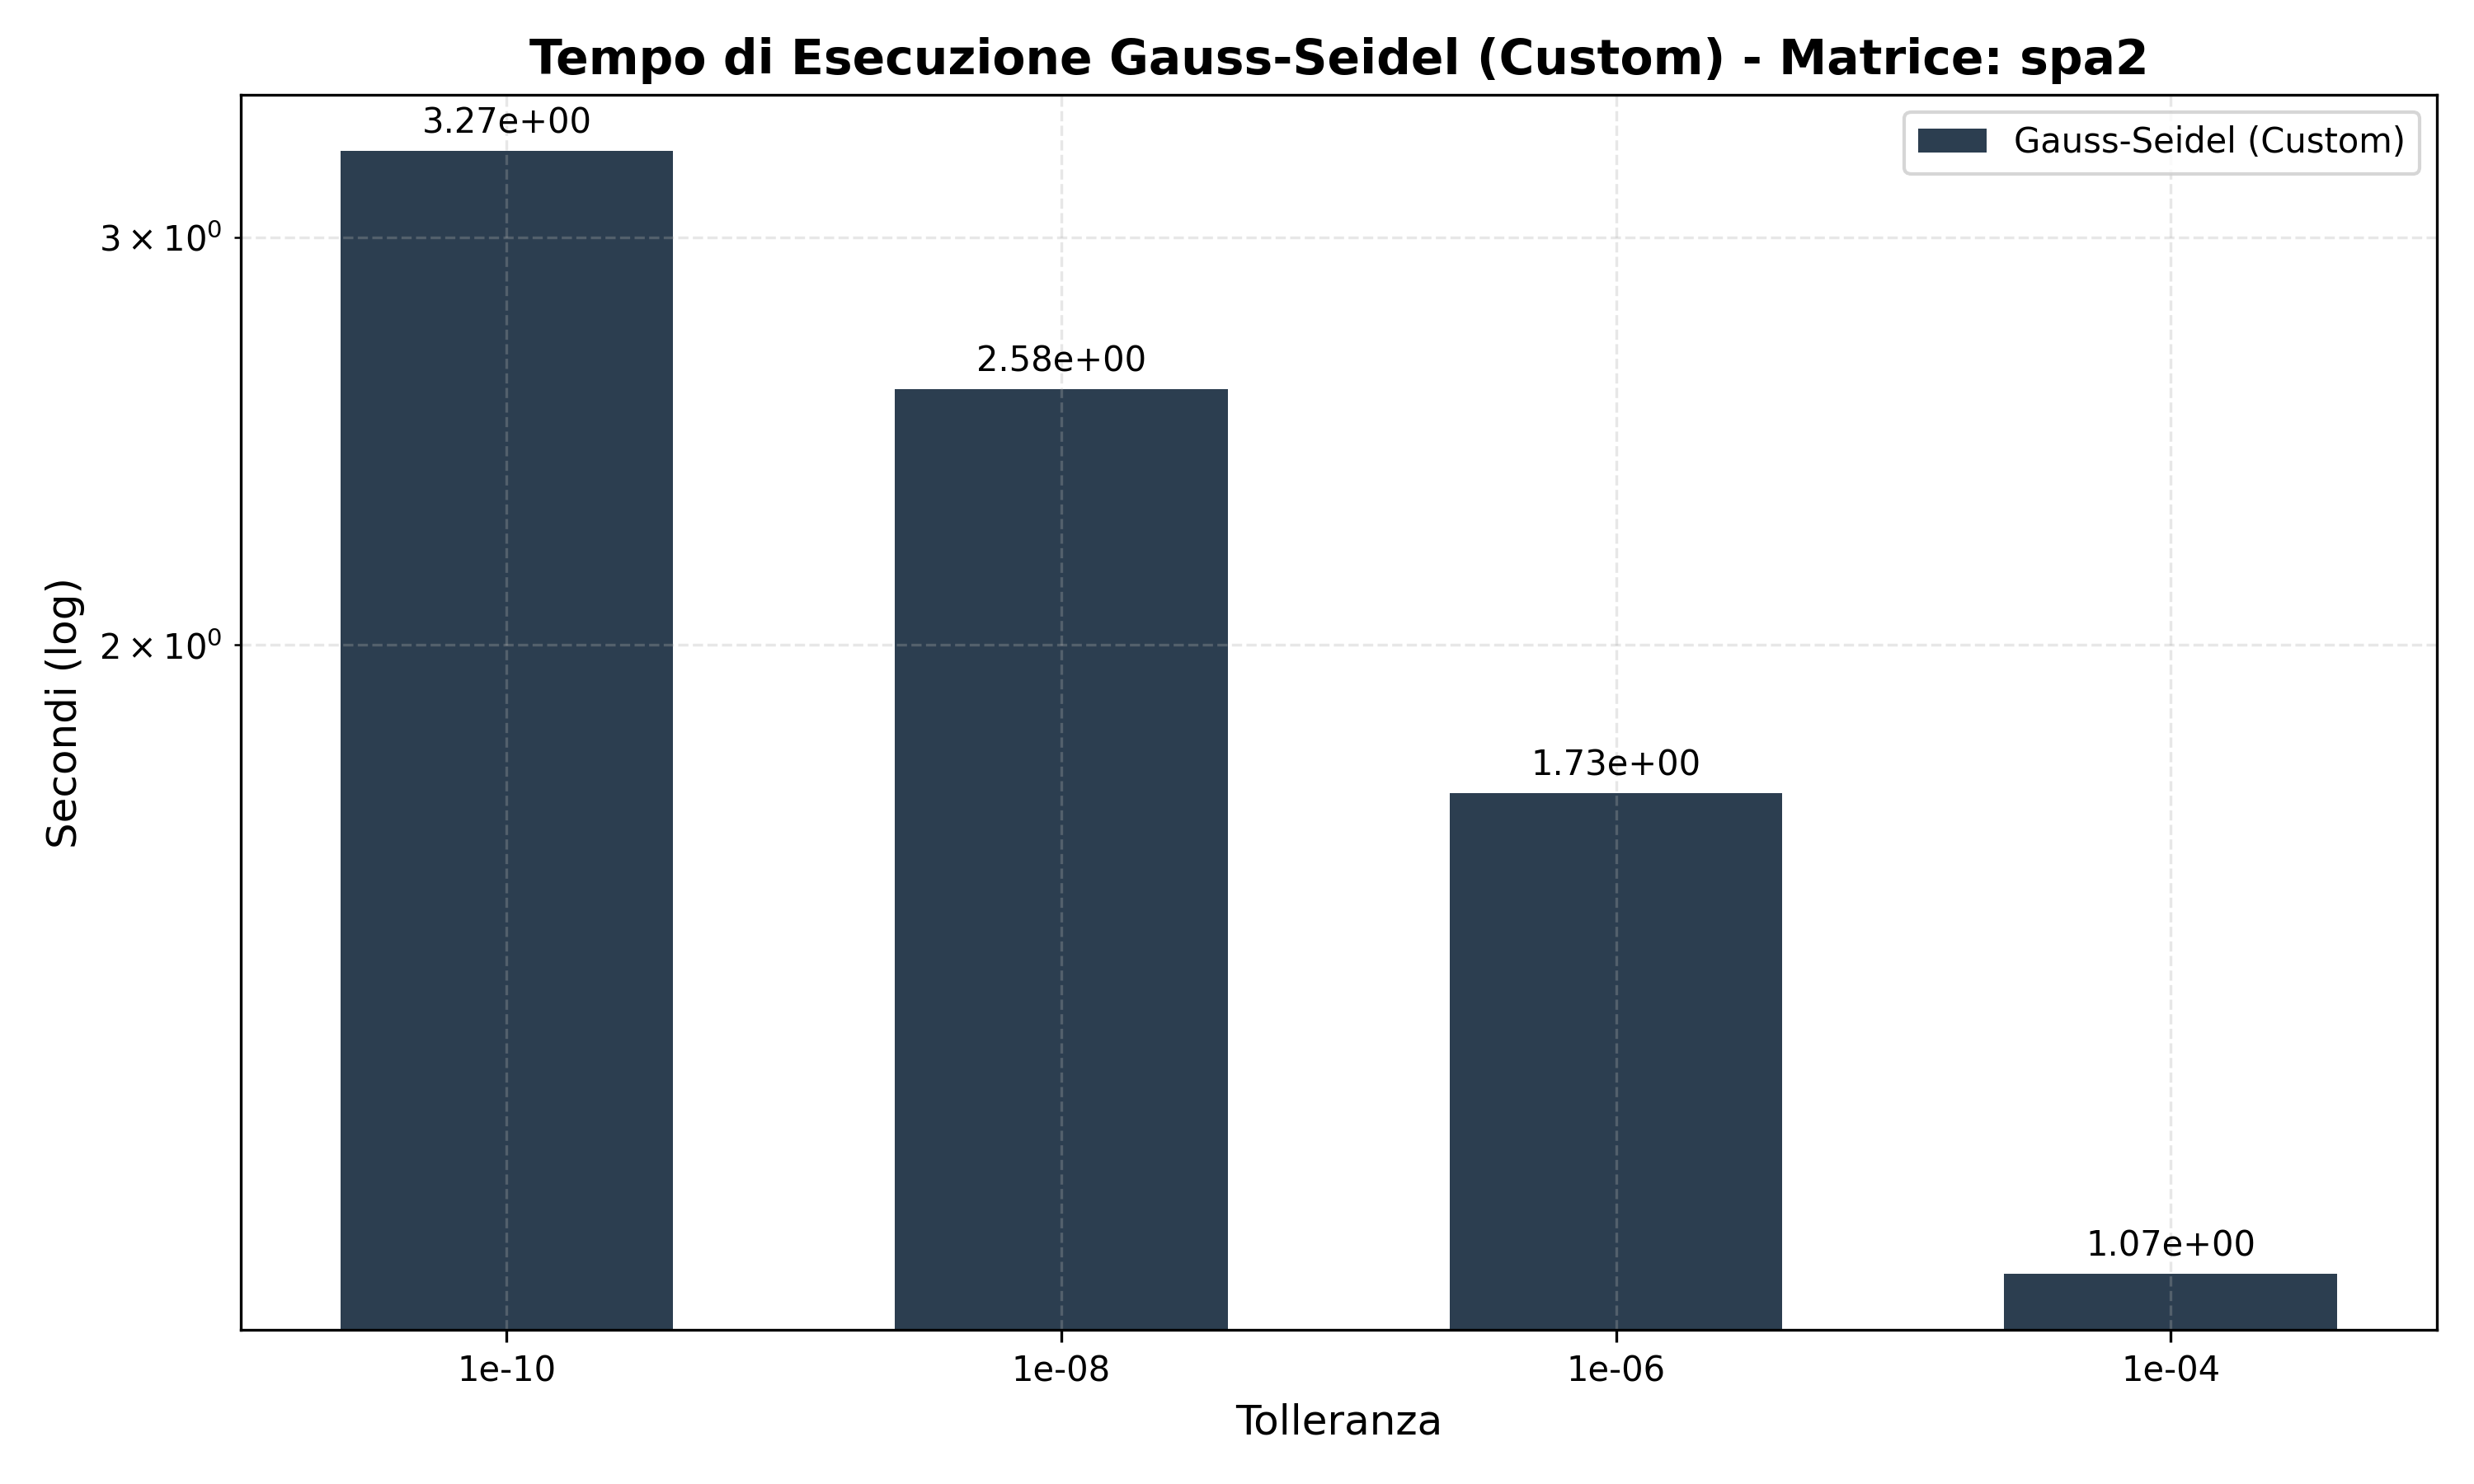
\includegraphics[width=\textwidth]{plots/gs_custom_spa2.png} % Da sostituire
        \caption{GS Custom (Forward Sub)}
    \end{minipage}\hfill
    \begin{minipage}{0.48\textwidth}
        \centering
        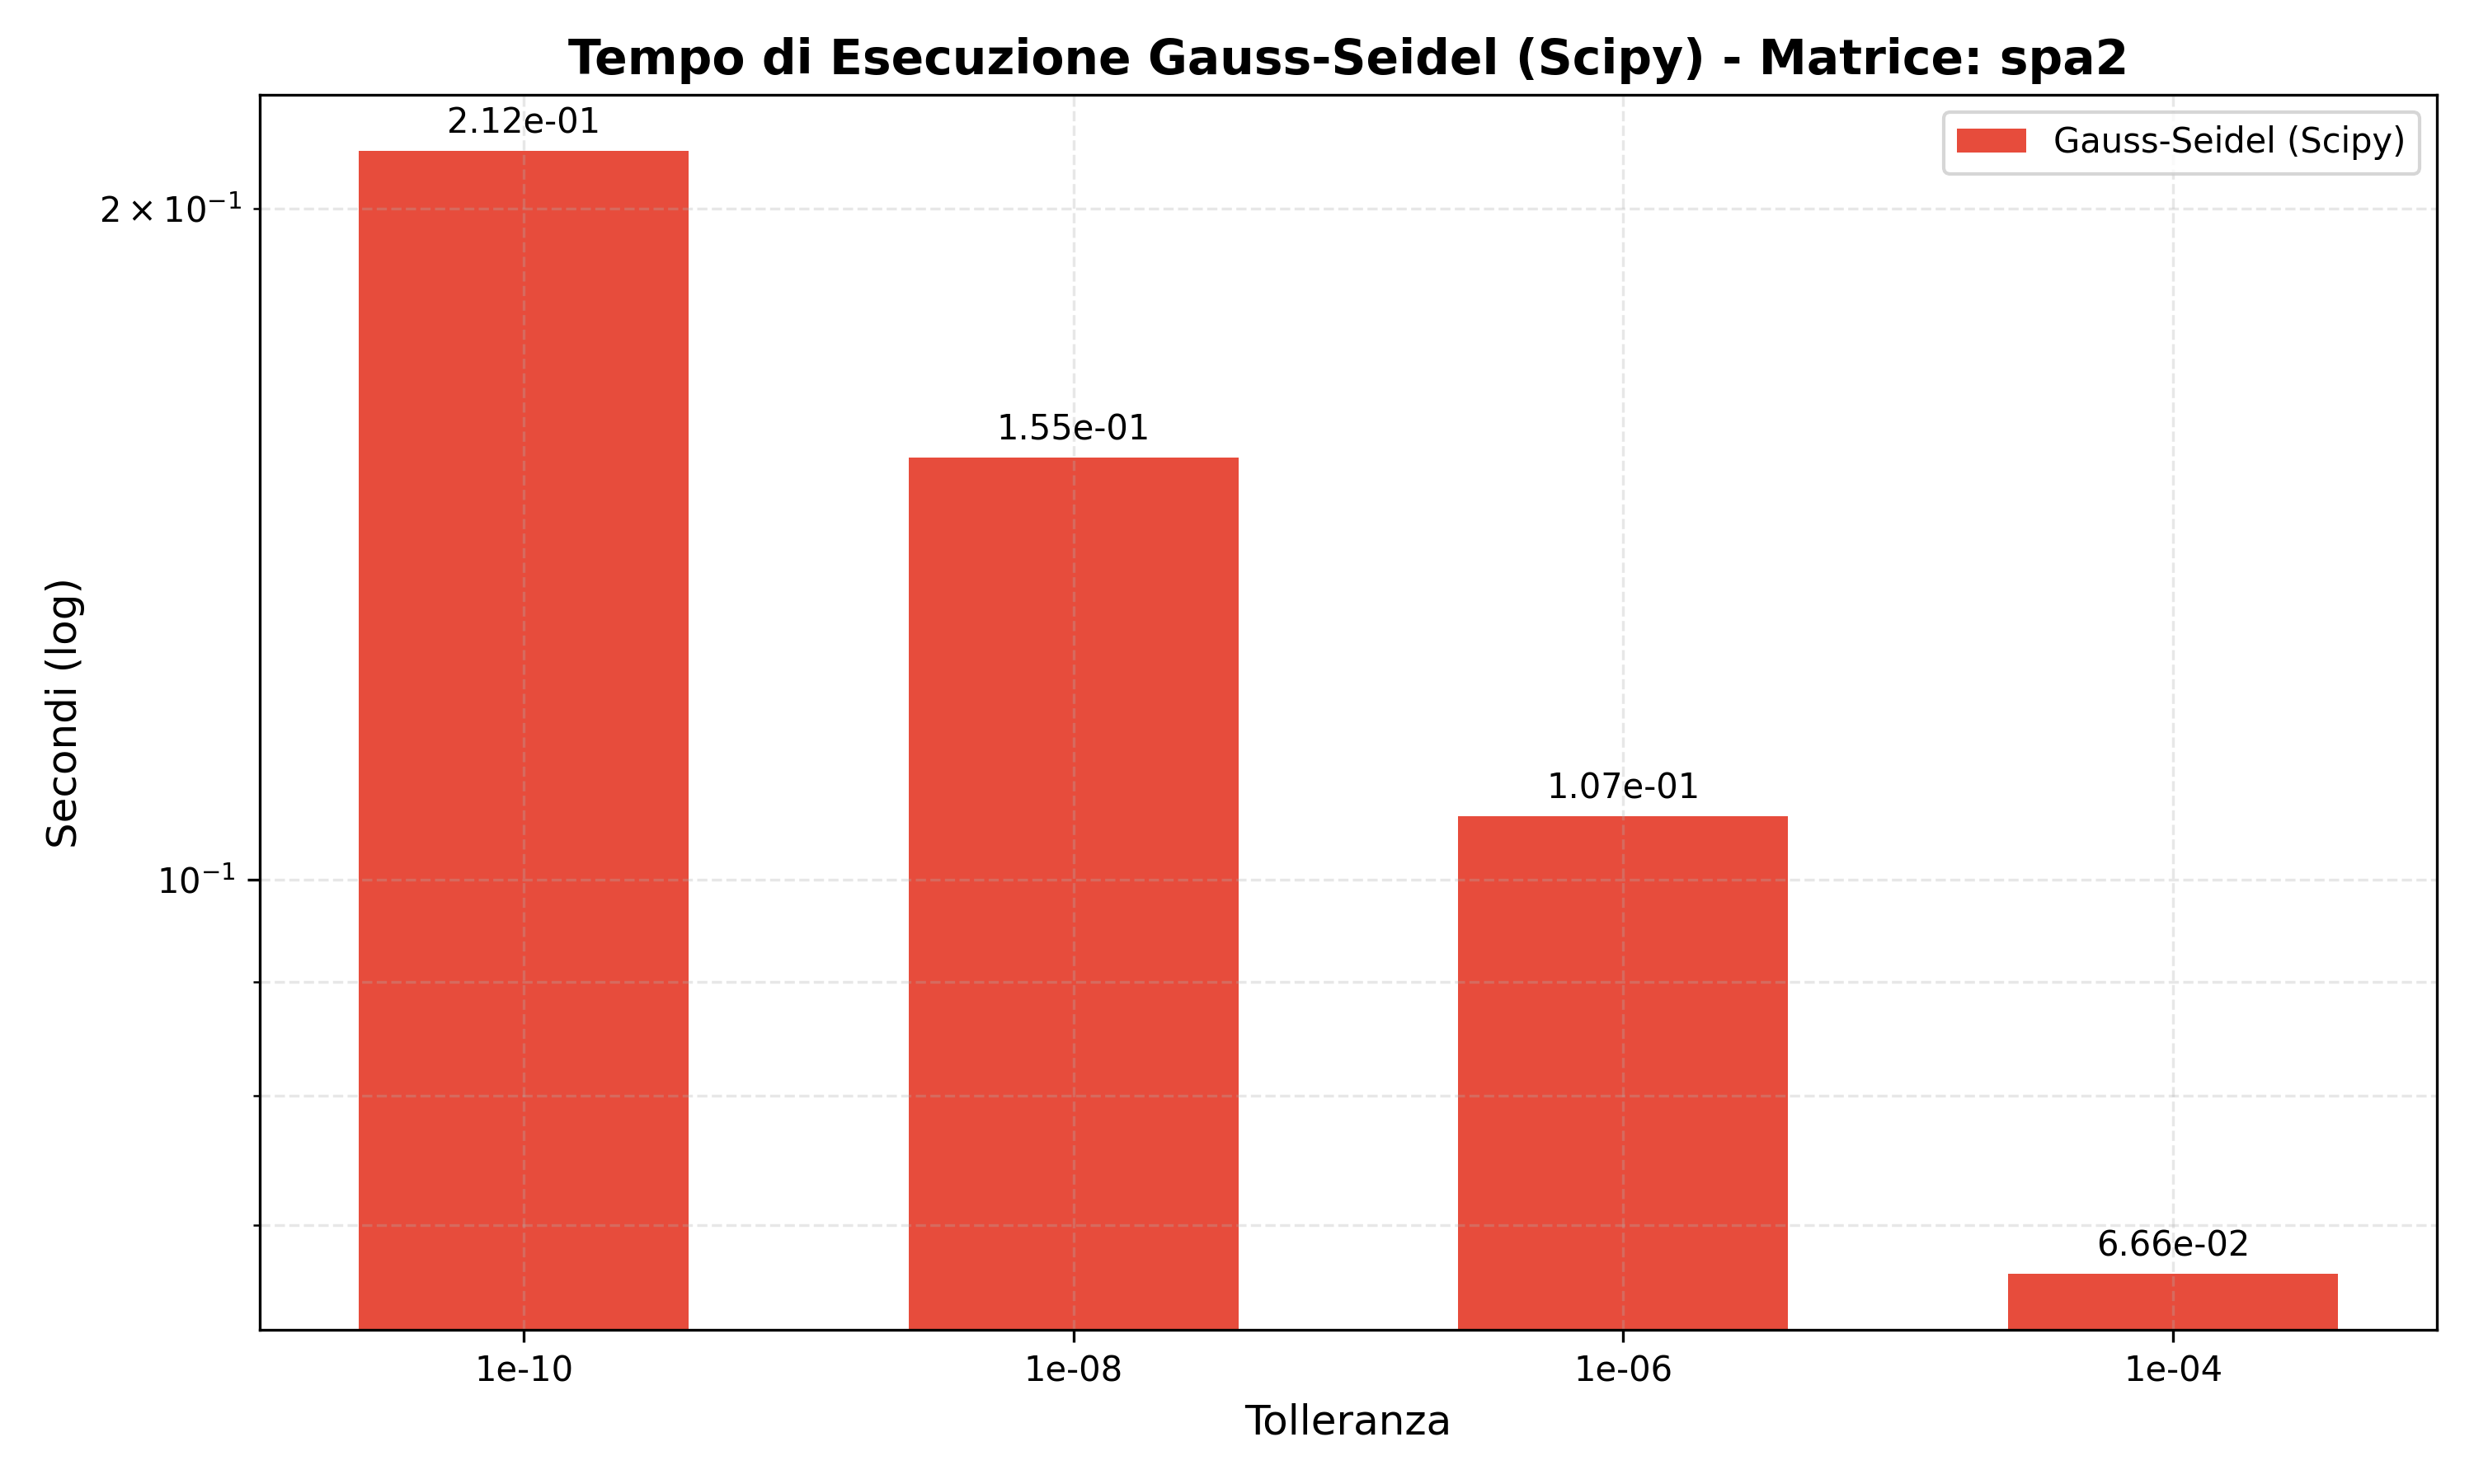
\includegraphics[width=\textwidth]{plots/gs_scipy_spa2.png} % Da sostituire
        \caption{GS SciPy (spsolve\_triangular)}
    \end{minipage}
\end{figure}

Come discusso nel capitolo precedente, è stato condotto un confronto diretto tra l'implementazione custom di sostituzione in avanti e la funzione ottimizzata in C offerta da SciPy (\texttt{spsolve\_triangular}). I grafici illustrano il tempo totale di esecuzione dell'algoritmo, e non quello della singola iterazione. A parità di iterazioni e di errore relativo, l'implementazione manuale mostra una notevole lentezza del loop nativo di Python rispetto alle funzioni pre-compilate della libreria.

\subsection{Analisi dell'Errore Relativo}
\begin{figure}[H]
    \centering
    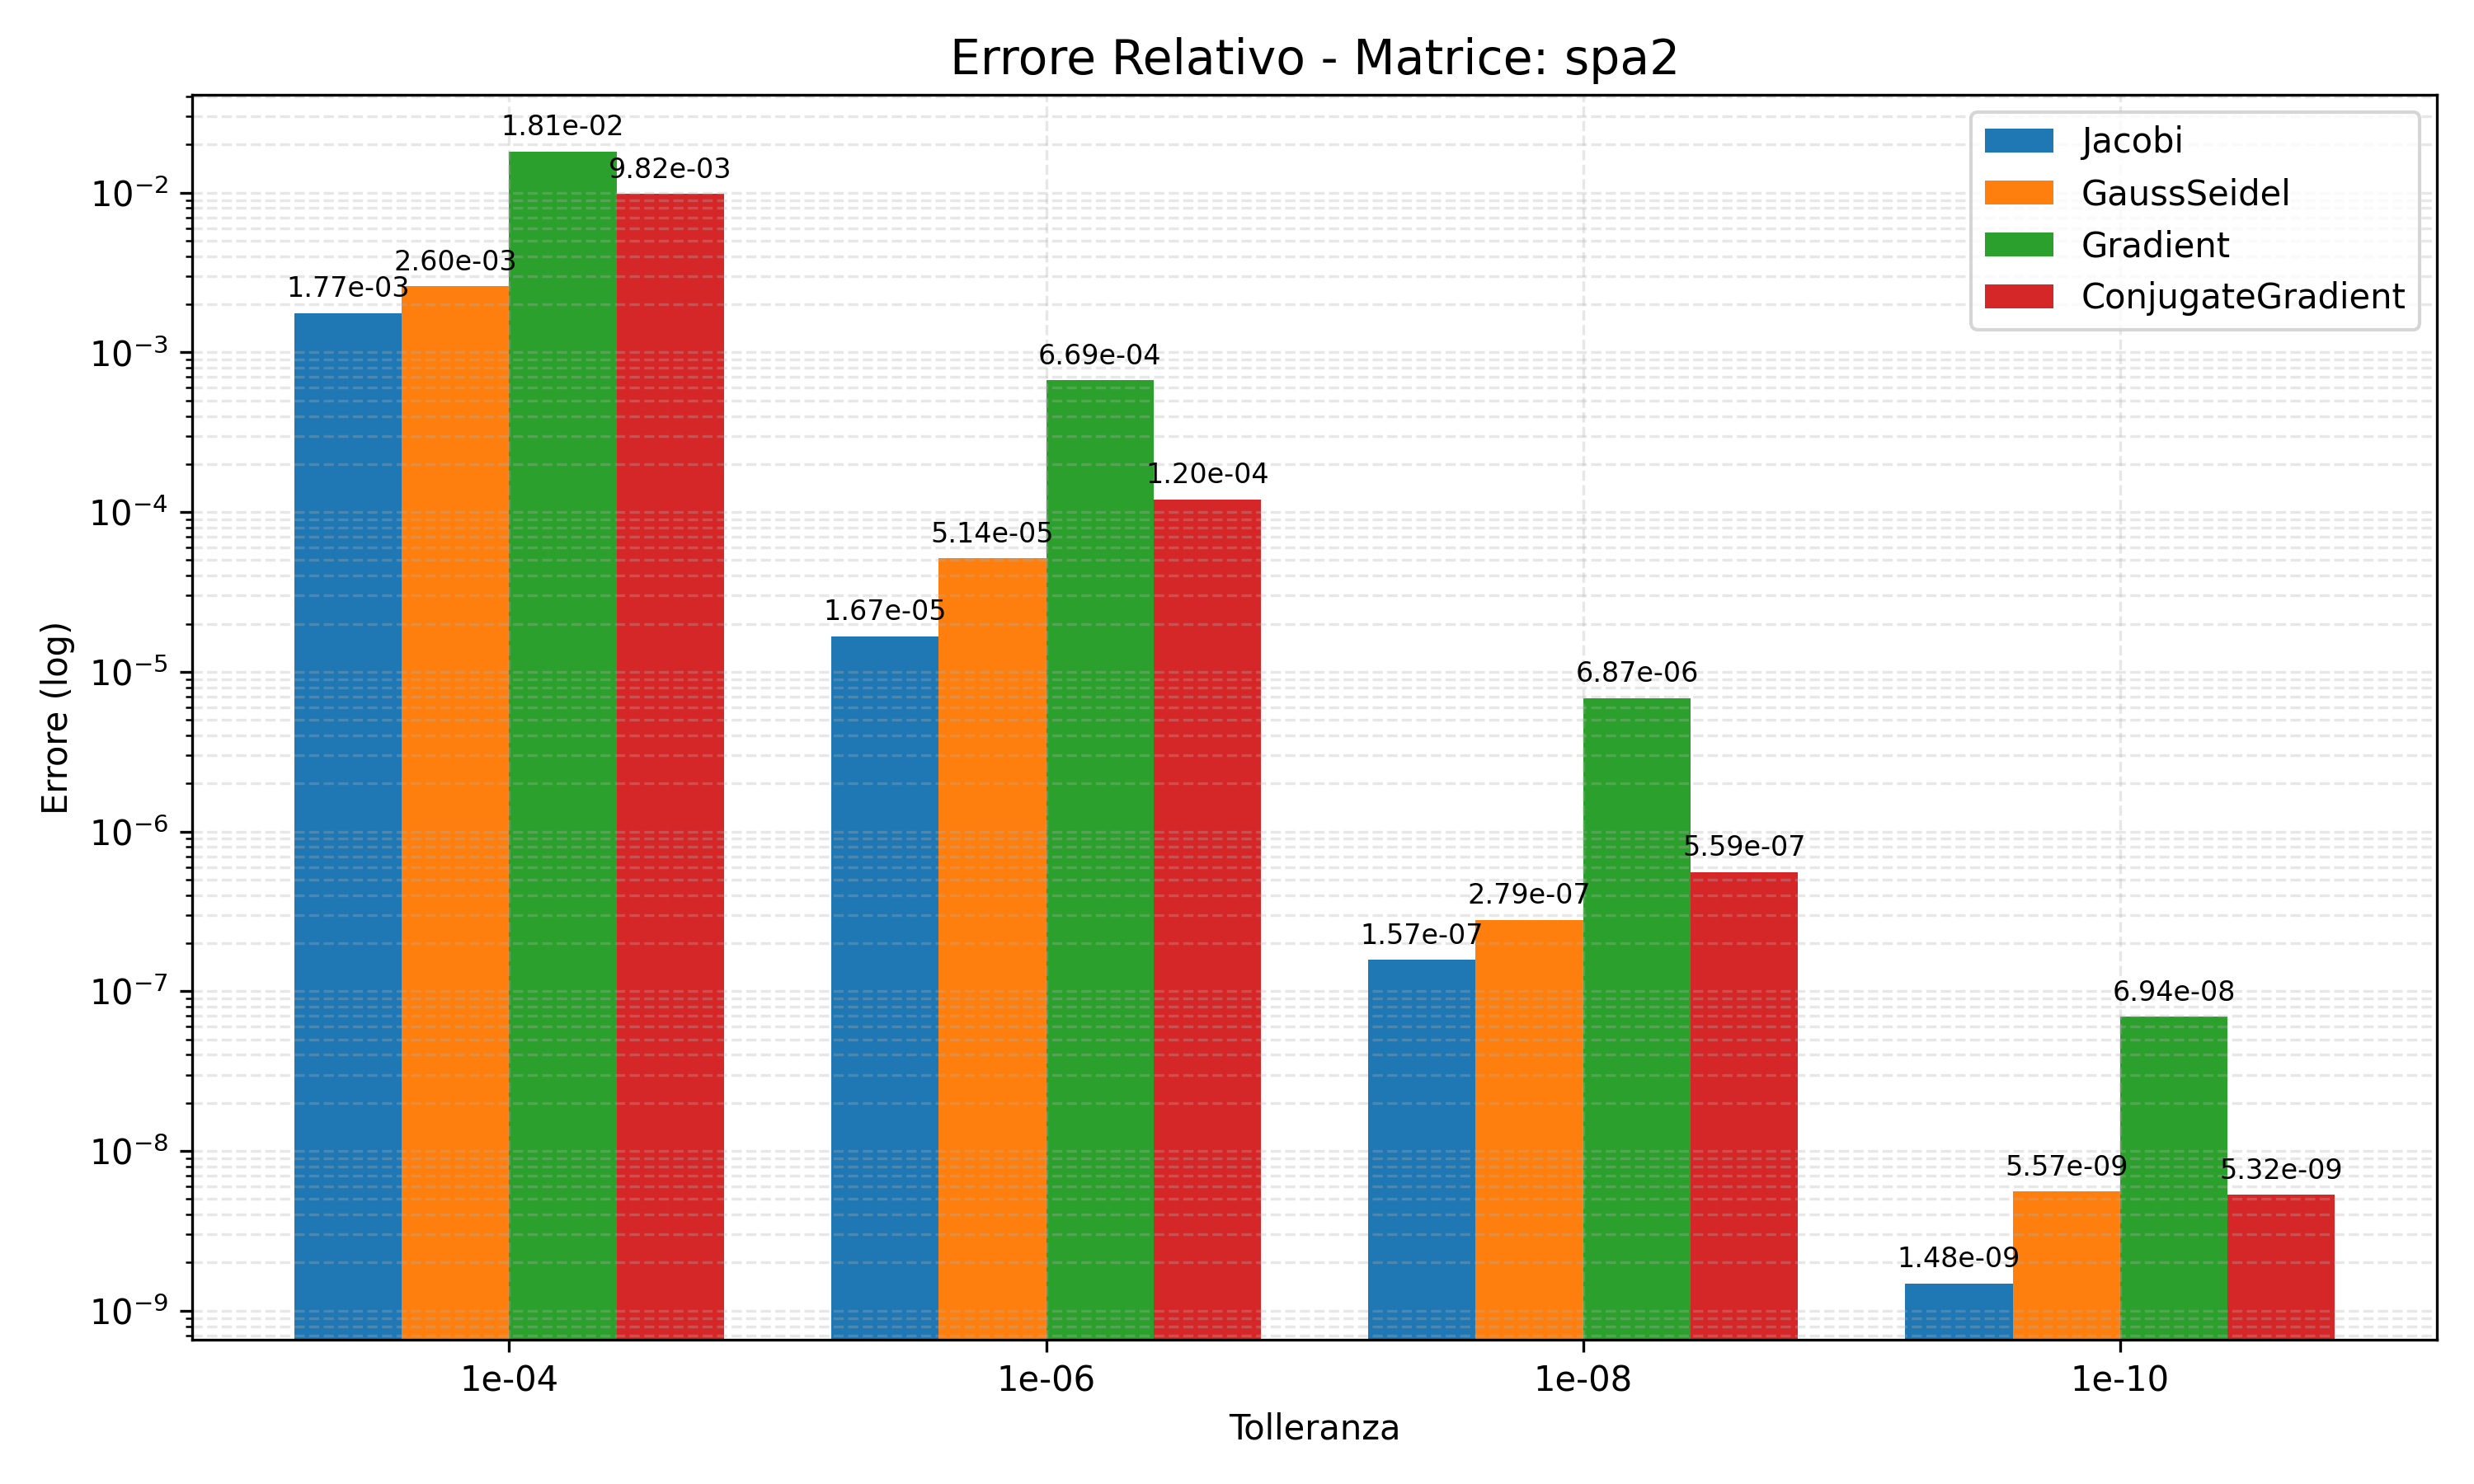
\includegraphics[width=0.9\textwidth]{plots/spa2_error.png}
    \caption{Errore relativo per spa2}
\end{figure}

Si nota che tutti i metodi riescono a soddisfare i requisiti decrescendo in modo costante. Il metodo di \textbf{Jacobi} raggiunge costantemente i valori di errore più bassi. Il metodo di \textbf{Gau\ss{}-Seidel} e il \textbf{Gradiente Coniugato} si alternano o si equivalgono nelle prestazioni: mentre a tolleranze alte Gau\ss{}-Seidel ottiene un errore leggermente inferiore, abbassando la soglia è il Gradiente Coniugato a risultare leggermente più preciso. Infine, il metodo del \textbf{Gradiente} standard registra sempre l'errore relativo più alto a convergenza.

\section{Matrice: vem1}
\subsection{Analisi della Matrice}
In questa sottosezione viene presentata l'analisi morfologica della matrice \texttt{vem1}. La tabella \ref{tab:analisi_vem1} ne riassume le caratteristiche strutturali, mentre la figura \ref{fig:heatmap_vem1} ne mostra la distribuzione dei valori tramite heatmap.

\begin{figure}[H]
    \centering
    % Prima colonna per la tabella
    \begin{minipage}[c]{0.48\textwidth}
        \centering
        \begin{tabular}{lr}
            \toprule
            \multicolumn{2}{l}{\textbf{Matrice vem1}} \\
            \midrule
            \textbf{Rows} & 1681 \\
            \textbf{Cols} & 1681 \\
            \textbf{Area} & 2825761 \\
            \textbf{Density (\%)} & 0.474 \\
            \textbf{Mean} & 0.0235 \\
            \textbf{Std Dev} & 1.08 \\
            \textbf{Condition Number} & 324.6 \\
            \bottomrule
        \end{tabular}
        \captionof{table}{Analisi vem1}
        \label{tab:analisi_vem1}
    \end{minipage}\hfill
    % Seconda colonna per l'immagine
    \begin{minipage}[c]{0.48\textwidth}
        \centering
        \includegraphics[width=\linewidth]{plots/vem1_heatmap.png}
        \captionof{figure}{Heatmap di vem1}
        \label{fig:heatmap_vem1}
    \end{minipage}
\end{figure}
La matrice \texttt{vem1} è estremamente sparsa (0.47\%) e presenta un numero di condizionamento molto basso (324.6). Questo la rende la matrice più "facile" tra quelle analizzate, e ci si aspetta che tutti i metodi raggiungano la convergenza in poche iterazioni.

\subsection{Risultati Numerici}
La seguente tabella riassume i risultati ottenuti per i quattro algoritmi al variare della tolleranza richiesta per la matrice \texttt{vem1}.

\begin{table}[H]
    \centering
    \begin{tabular}{|c|c|c|c|c|}
        \hline
        \textbf{Tol} & \textbf{Metodo} & \textbf{Numero iterazioni} & \textbf{Tempo (s)} & \textbf{Errore relativo} \\
        \hline
        $10^{-4}$ & Jacobi & 1314 & 0.0272 & $3.54 \cdot 10^{-3}$ \\
                  & Gauss-Seidel & 659 & 1.8199 & $3.51 \cdot 10^{-3}$ \\
                  & Gradient & 890 & 0.0228 & $2.70 \cdot 10^{-3}$ \\
                  & Conjugate Gradient & 38 & 0.0009 & $4.08 \cdot 10^{-5}$ \\
        \hline
        $10^{-6}$ & Jacobi & 2433 & 0.0423 & $3.54 \cdot 10^{-5}$ \\
                  & Gauss-Seidel & 1218 & 3.2280 & $3.53 \cdot 10^{-5}$ \\
                  & Gradient & 1612 & 0.0351 & $2.71 \cdot 10^{-5}$ \\
                  & Conjugate Gradient & 45 & 0.0014 & $3.73 \cdot 10^{-7}$ \\
        \hline
        $10^{-8}$ & Jacobi & 3552 & 0.0668 & $3.54 \cdot 10^{-7}$ \\
                  & Gauss-Seidel & 1778 & 4.7280 & $3.52 \cdot 10^{-7}$ \\
                  & Gradient & 2336 & 0.0487 & $2.70 \cdot 10^{-7}$ \\
                  & Conjugate Gradient & 53 & 0.0011 & $2.83 \cdot 10^{-9}$ \\
        \hline
        $10^{-10}$ & Jacobi & 4671 & 0.0878 & $3.54 \cdot 10^{-9}$ \\
                  & Gauss-Seidel & 2338 & 6.2791 & $3.51 \cdot 10^{-9}$ \\
                  & Gradient & 3058 & 0.0667 & $2.71 \cdot 10^{-9}$ \\
                  & Conjugate Gradient & 59 & 0.0013 & $2.19 \cdot 10^{-11}$ \\
        \hline
    \end{tabular}
    \caption{Risultati numerici per vem1}
\end{table}

\subsection{Analisi delle Iterazioni}
\begin{figure}[H]
    \centering
    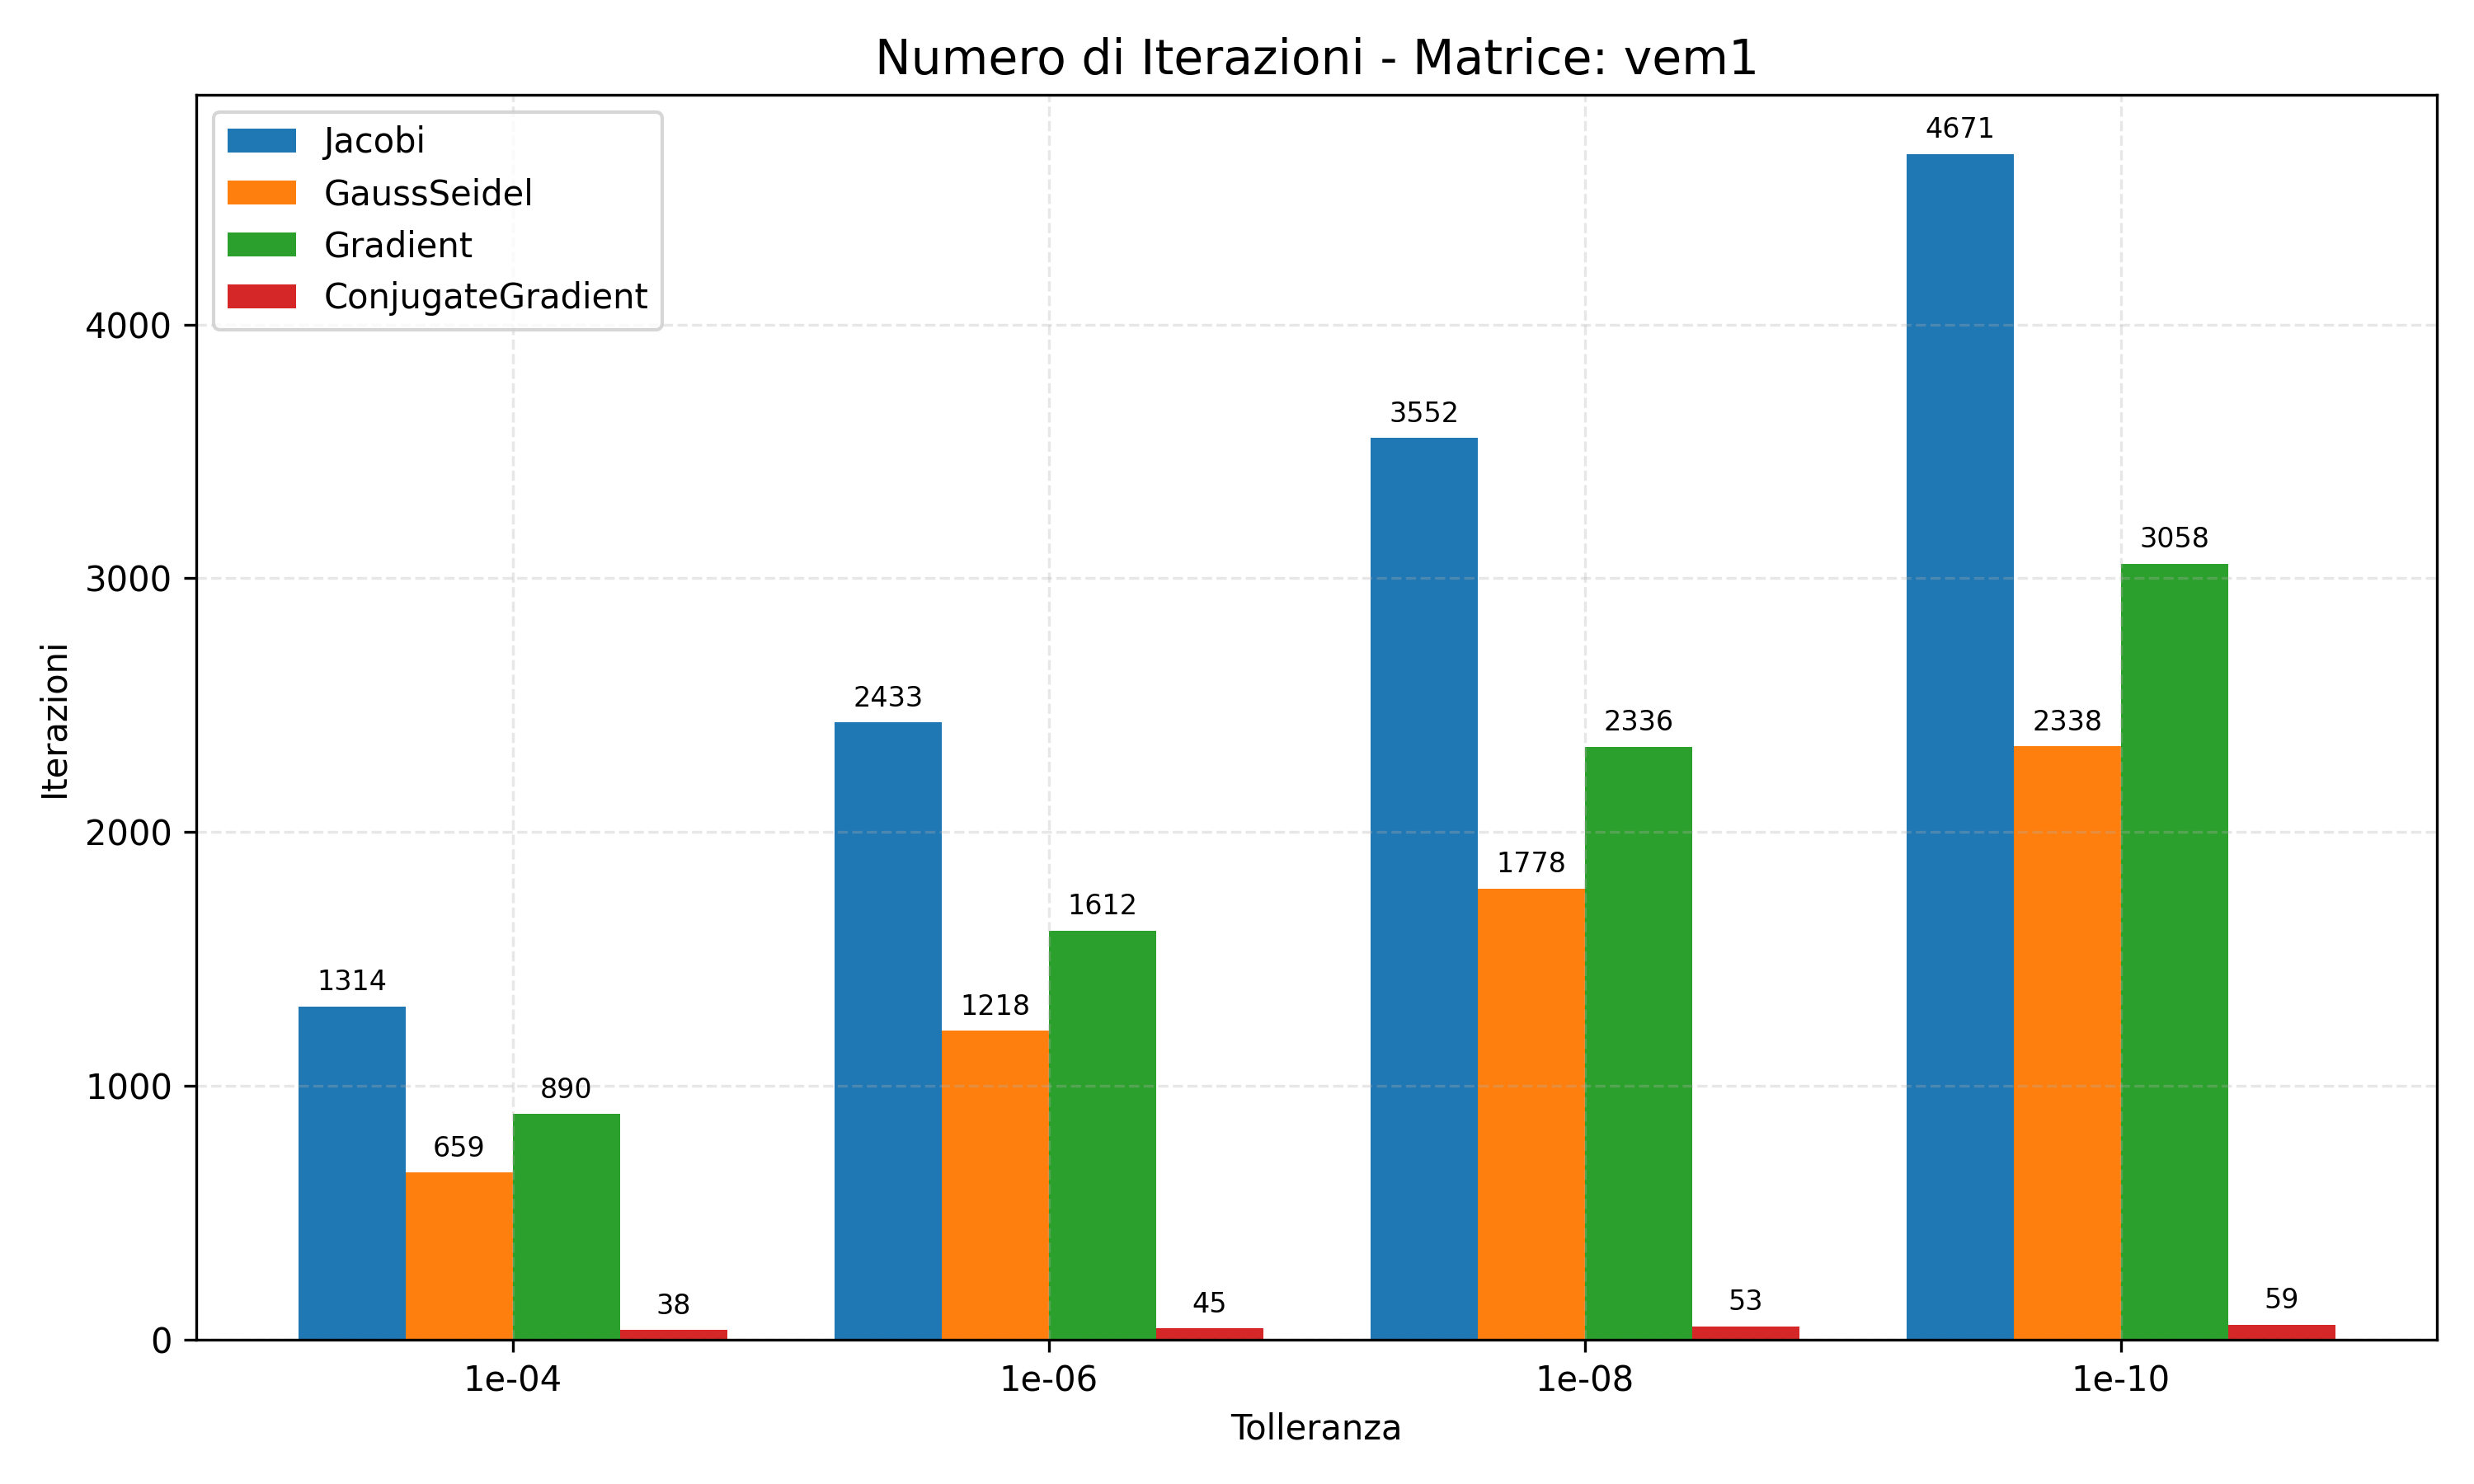
\includegraphics[width=0.9\textwidth]{plots/vem1_iterations.png}
    \caption{Numero di iterazioni per vem1}
\end{figure}

Il \textbf{Gradiente Coniugato} si conferma il più veloce, convergendo in pochissimi passi grazie al basso numero di condizionamento della matrice. \textbf{Jacobi} risulta invece il metodo più lento in assoluto, richiedendo migliaia di iterazioni. \textbf{Gau\ss{}-Seidel} e il \textbf{Gradiente} standard si collocano su valori intermedi, con Gau\ss{}-Seidel che mantiene un leggero vantaggio. Questo comportamento è molto diverso da quanto osservato nelle matrici precedenti, dove erano invece i metodi stazionari a convergere più rapidamente.

\subsection{Analisi dei Tempi}
\begin{figure}[H]
    \centering
    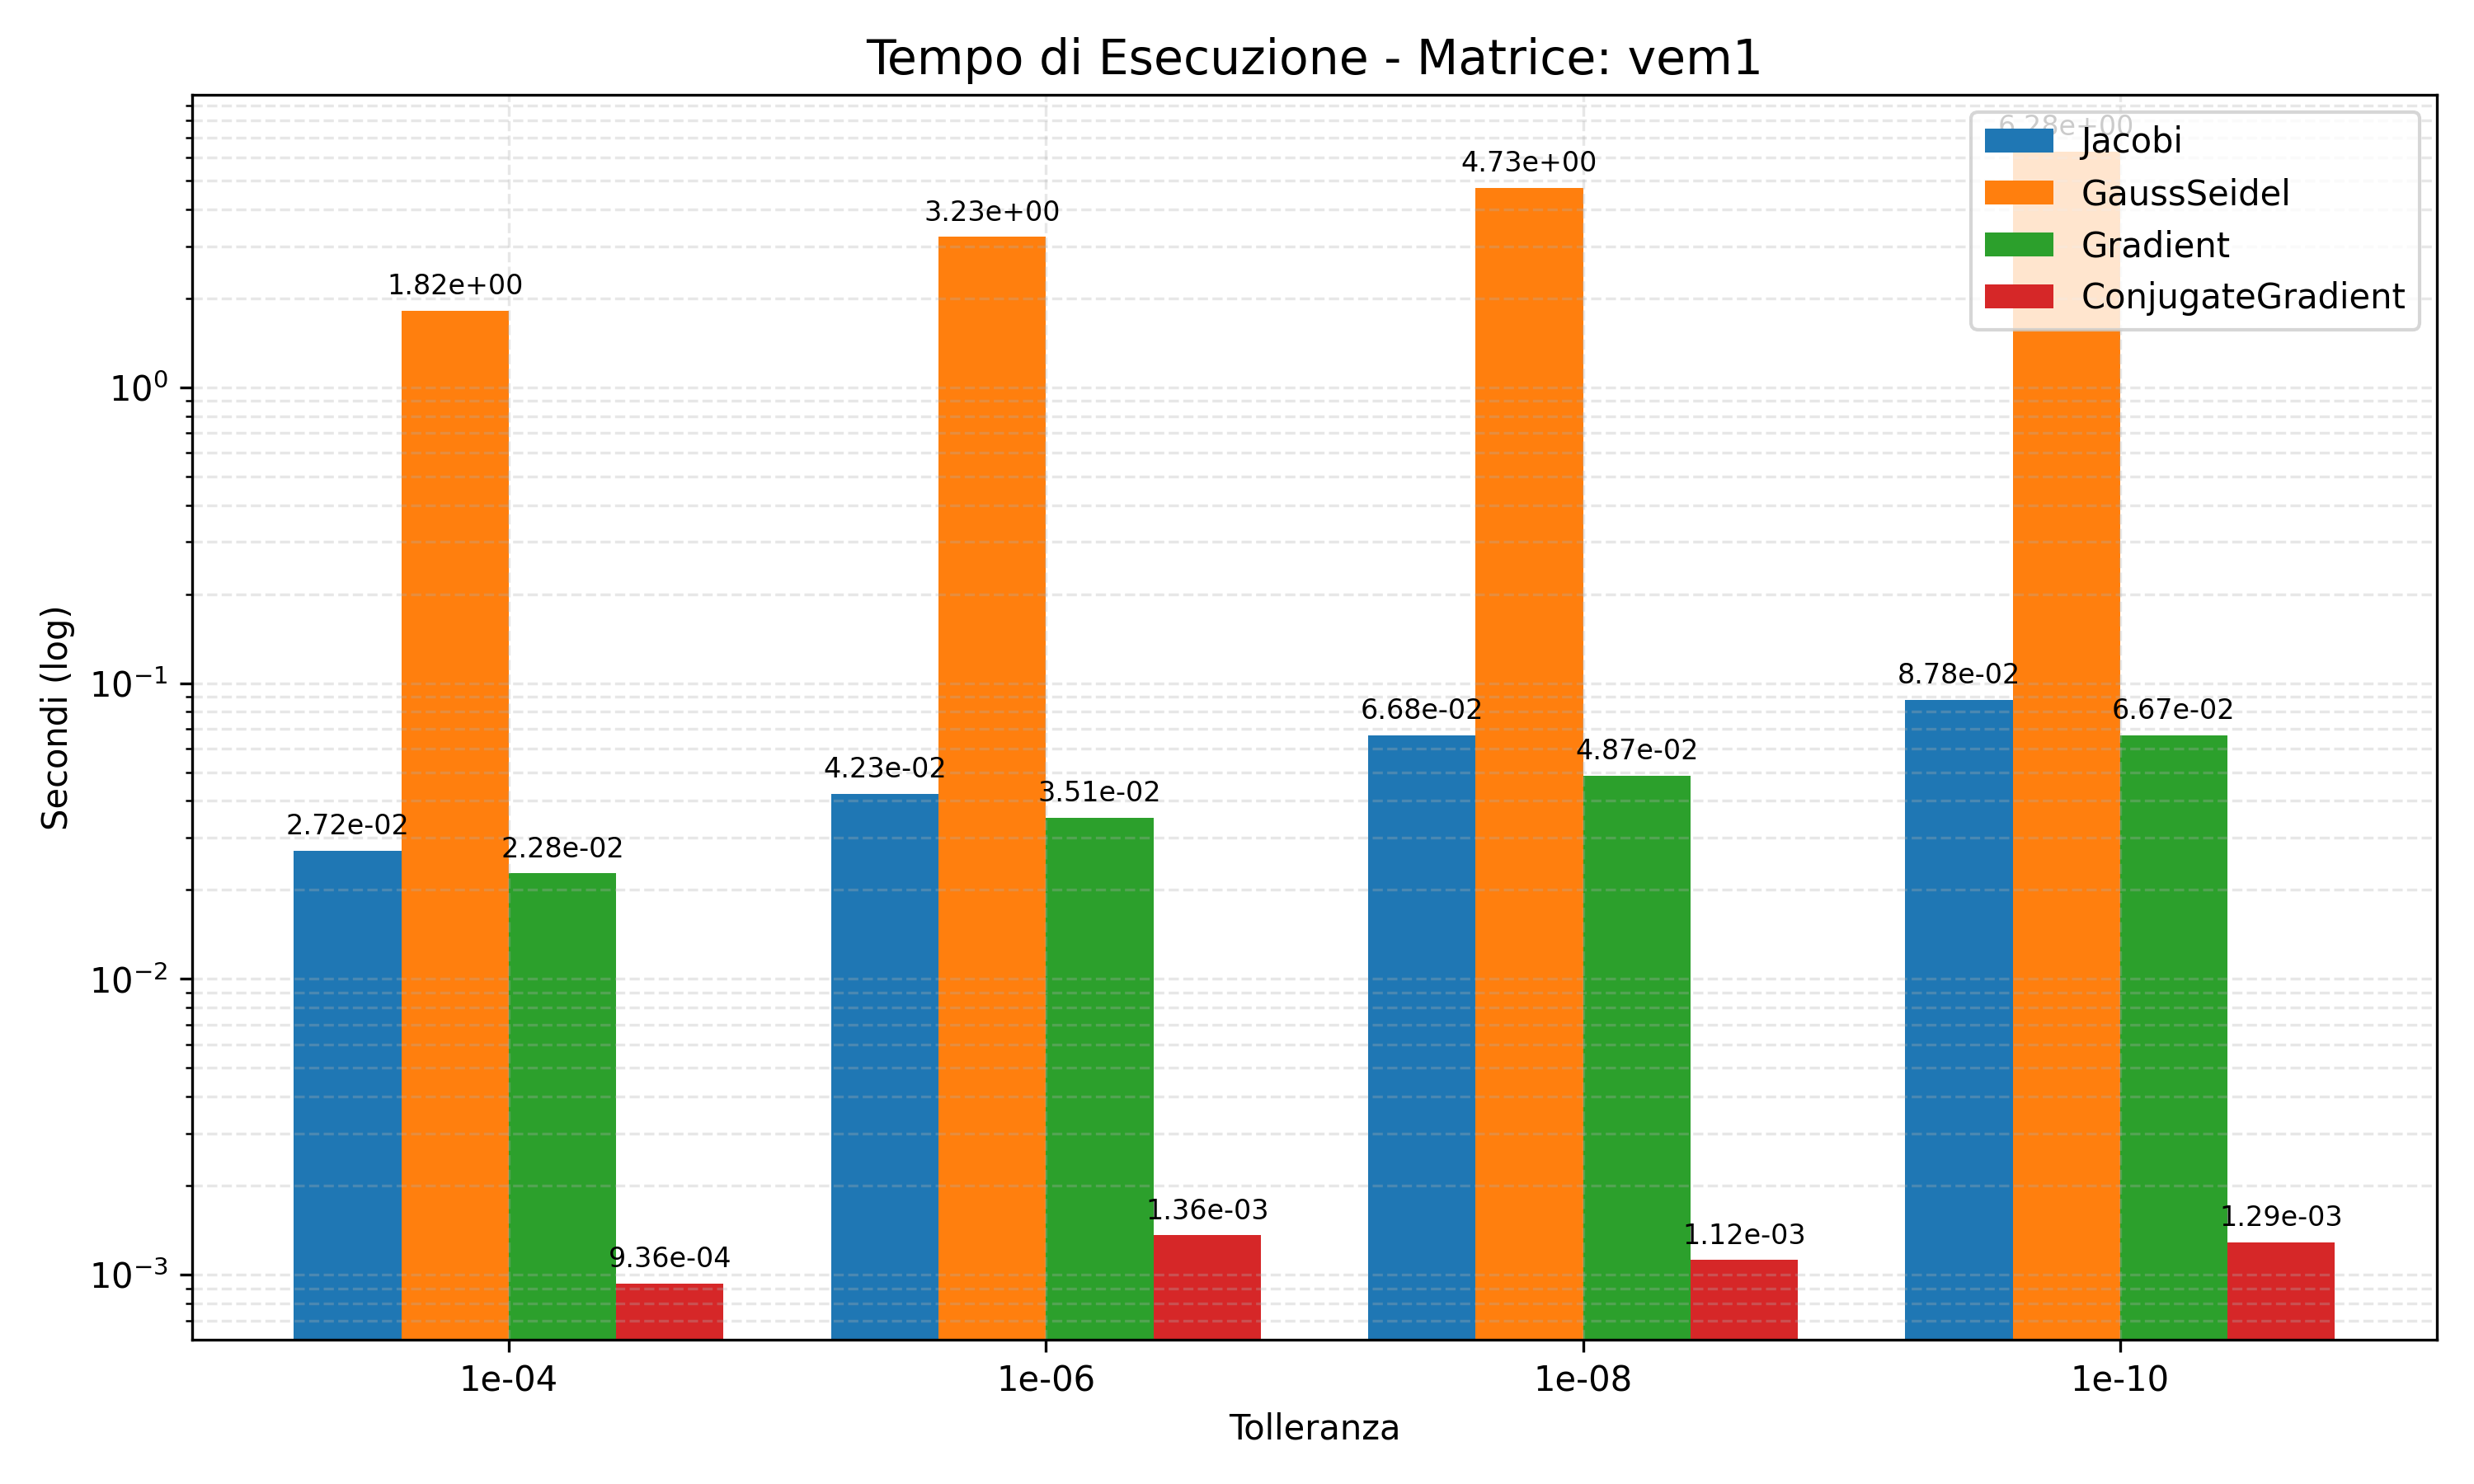
\includegraphics[width=0.9\textwidth]{plots/vem1_time.png}
    \caption{Tempo di esecuzione per vem1}
\end{figure}

Analizzando invece i tempi di esecuzione, il \textbf{Gradiente Coniugato} si conferma l'algoritmo più veloce in assoluto, coerentemente con il basso numero di iterazioni richieste. \textbf{Jacobi} e il \textbf{Gradiente} seguono a distanza ravvicinata, mentre \textbf{Gau\ss{}-Seidel} risulta invece il più lento, superando persino il \textbf{Gradiente} nonostante il minor numero di iterazioni. Questa discrepanza, ancor più marcata rispetto alle matrici precedenti, è da imputare nuovamente all'utilizzo della funzione custom per la risoluzione del sistema triangolare inferiore.

\subsection{Confronto Implementazioni Gauß-Seidel}
\begin{figure}[H]
    \centering
    \begin{minipage}{0.5\textwidth}
        \centering
        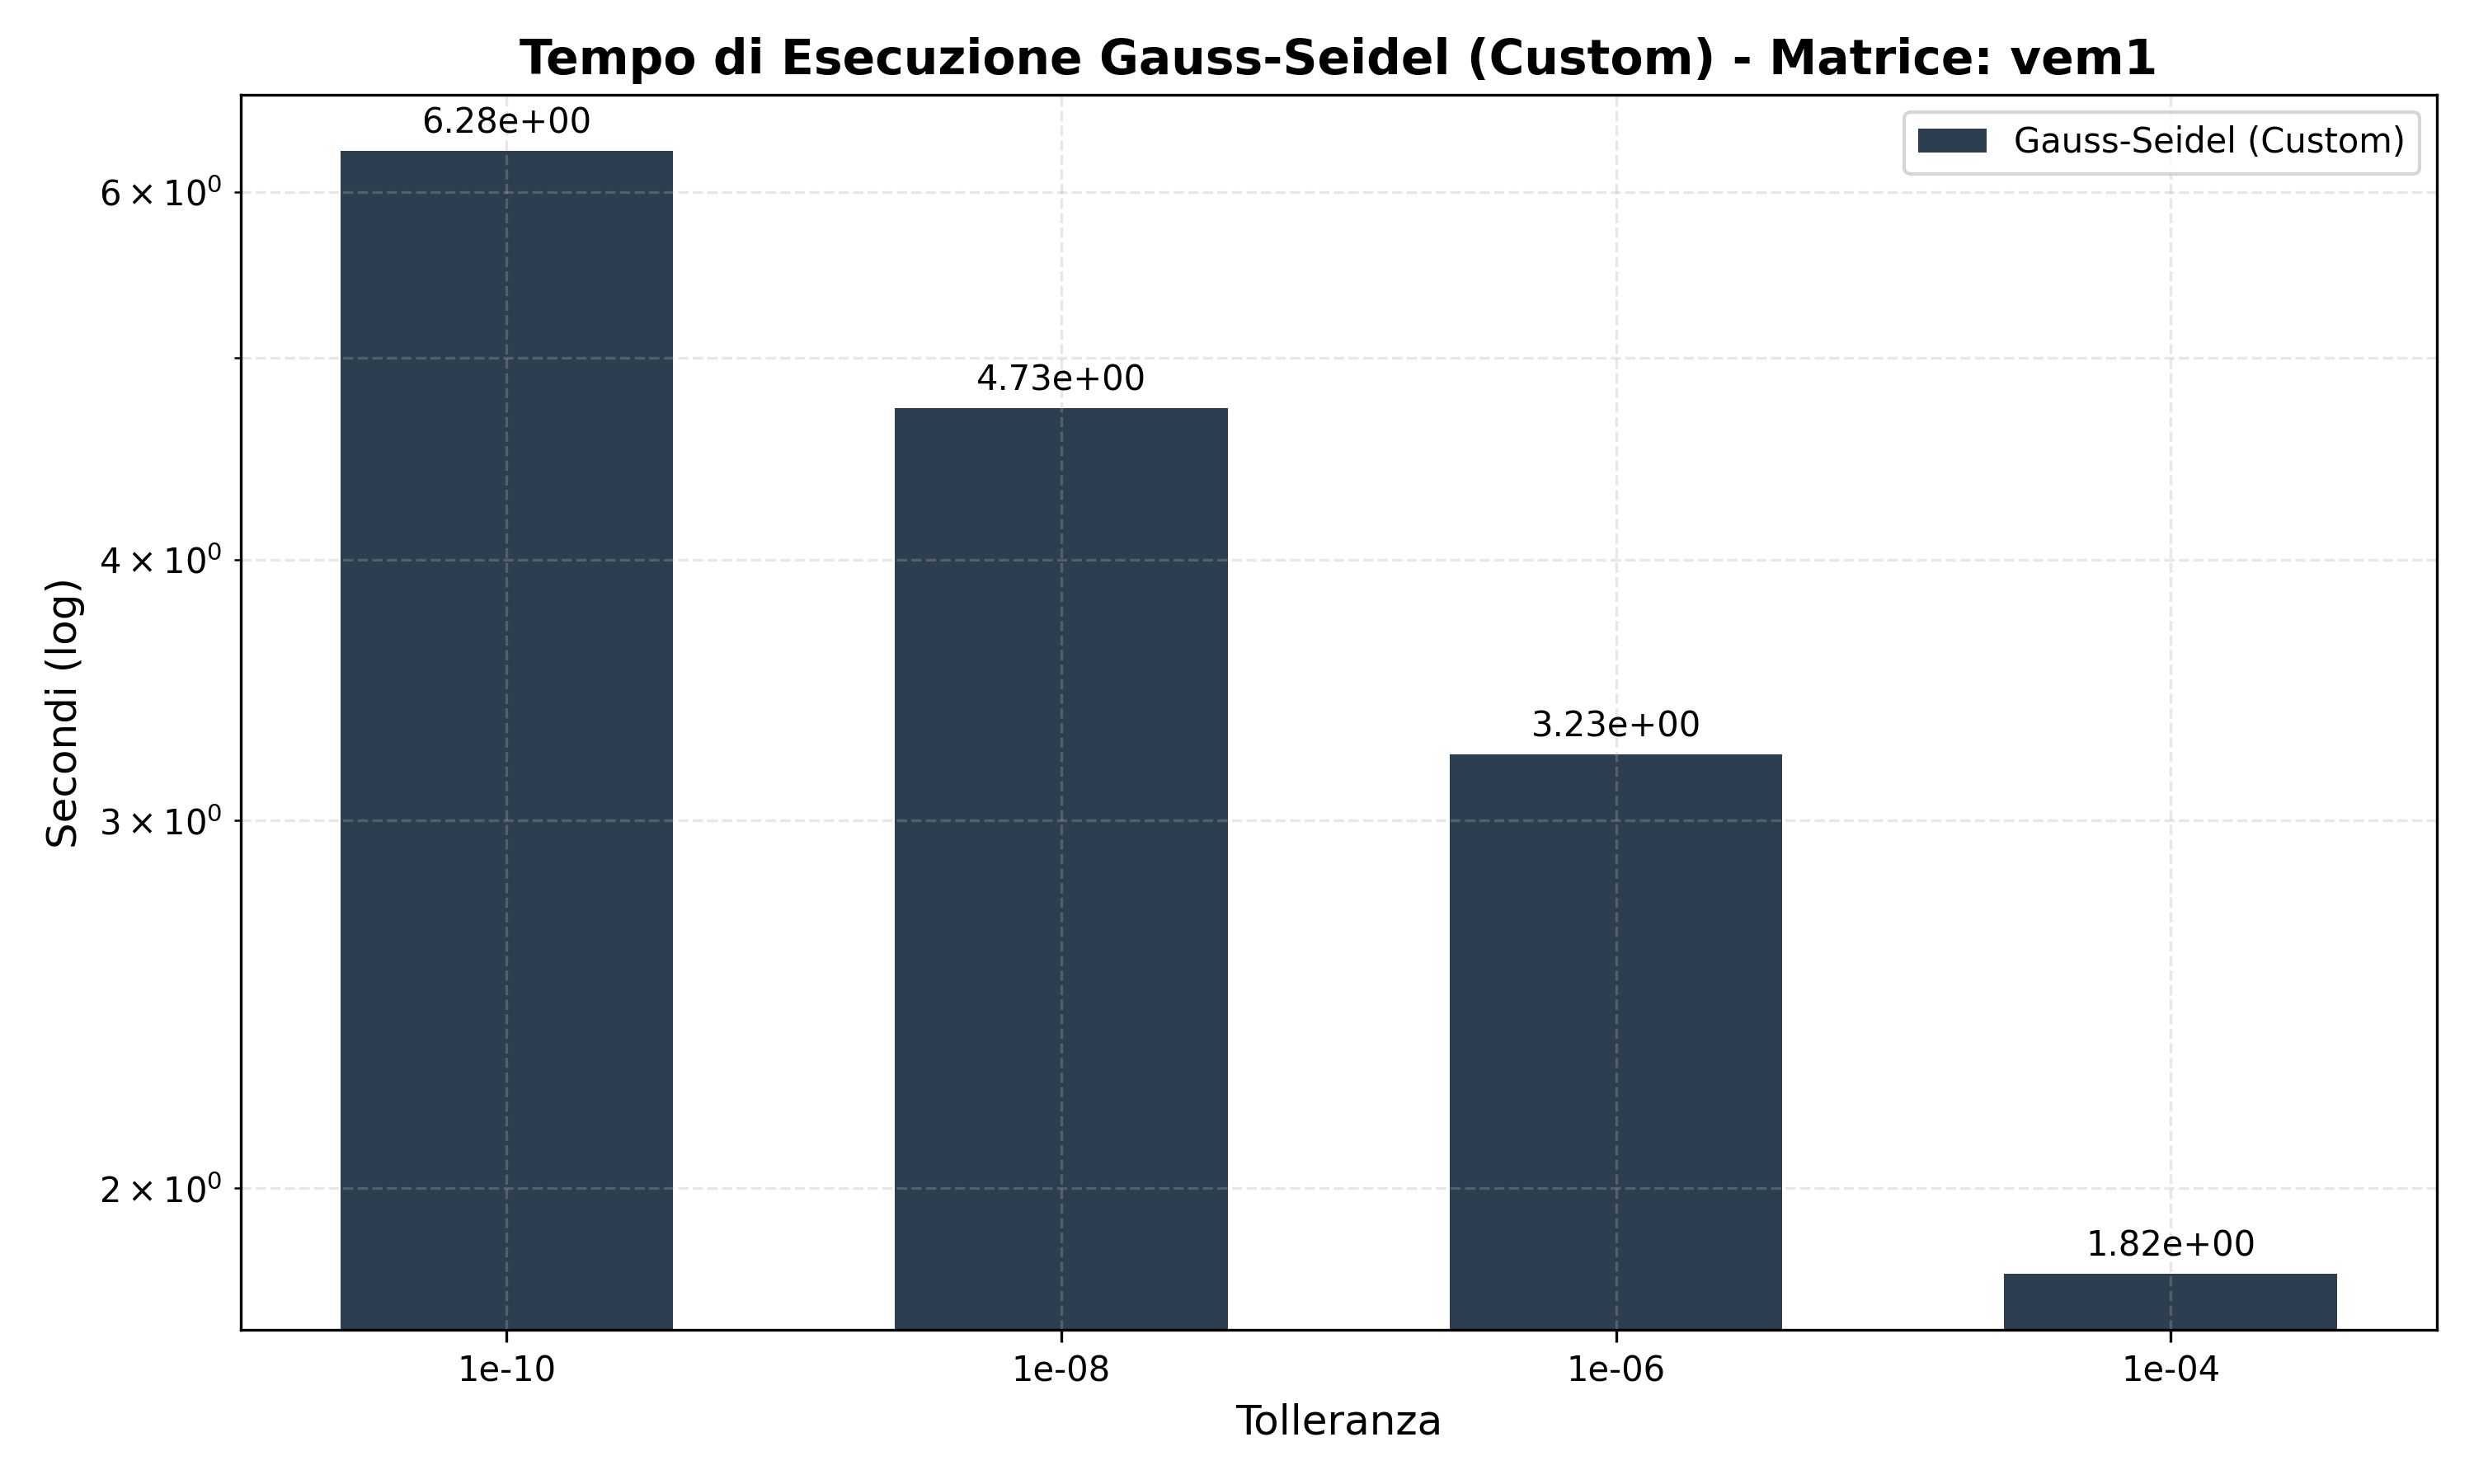
\includegraphics[width=\textwidth]{plots/gs_custom_vem1.png} % Da sostituire
        \caption{GS Custom (Forward Sub)}
    \end{minipage}\hfill
    \begin{minipage}{0.5\textwidth}
        \centering
        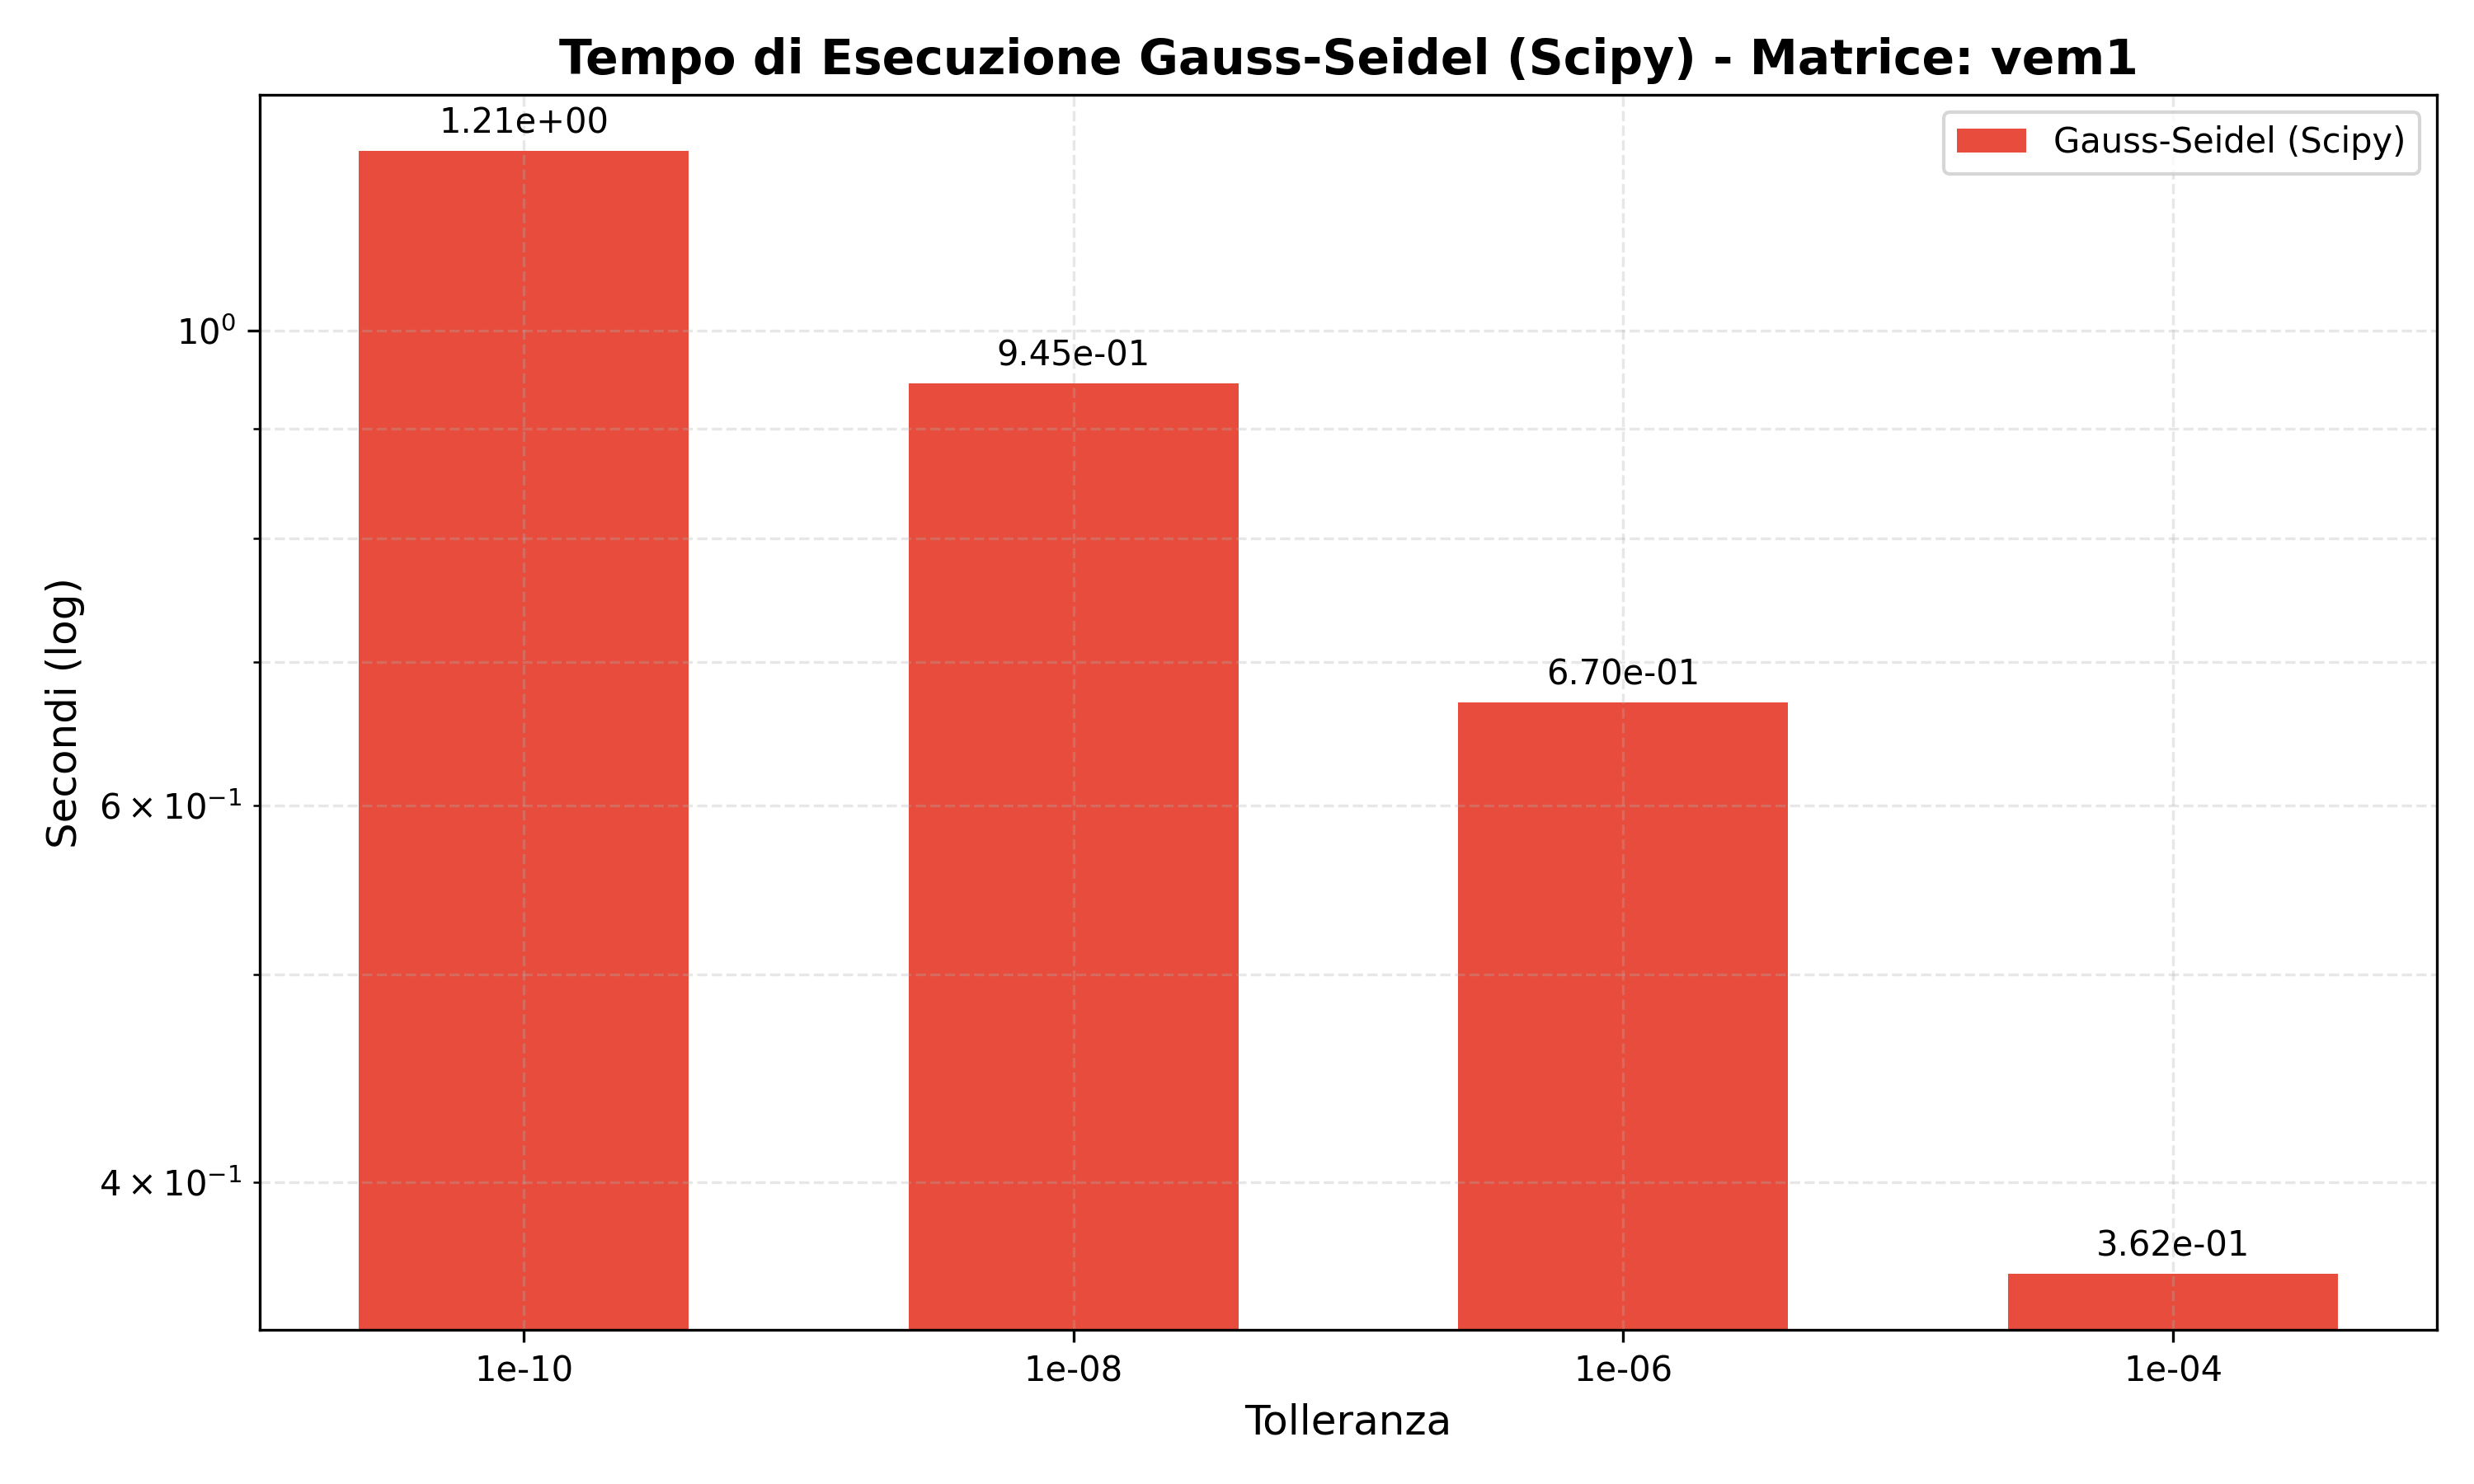
\includegraphics[width=\textwidth]{plots/gs_scipy_vem1.png} % Da sostituire
        \caption{GS SciPy (spsolve\_triangular)}
    \end{minipage}
\end{figure}

Come discusso nel capitolo precedente, è stato condotto un confronto diretto tra l'implementazione custom di sostituzione in avanti e la funzione ottimizzata in C offerta da SciPy (\texttt{spsolve\_triangular}). I grafici illustrano il tempo totale di esecuzione dell'algoritmo, e non quello della singola iterazione. A parità di iterazioni e di errore relativo, l'implementazione manuale mostra una notevole lentezza del loop nativo di Python rispetto alle funzioni pre-compilate della libreria.

\subsection{Analisi dell'Errore Relativo}
\begin{figure}[H]
    \centering
    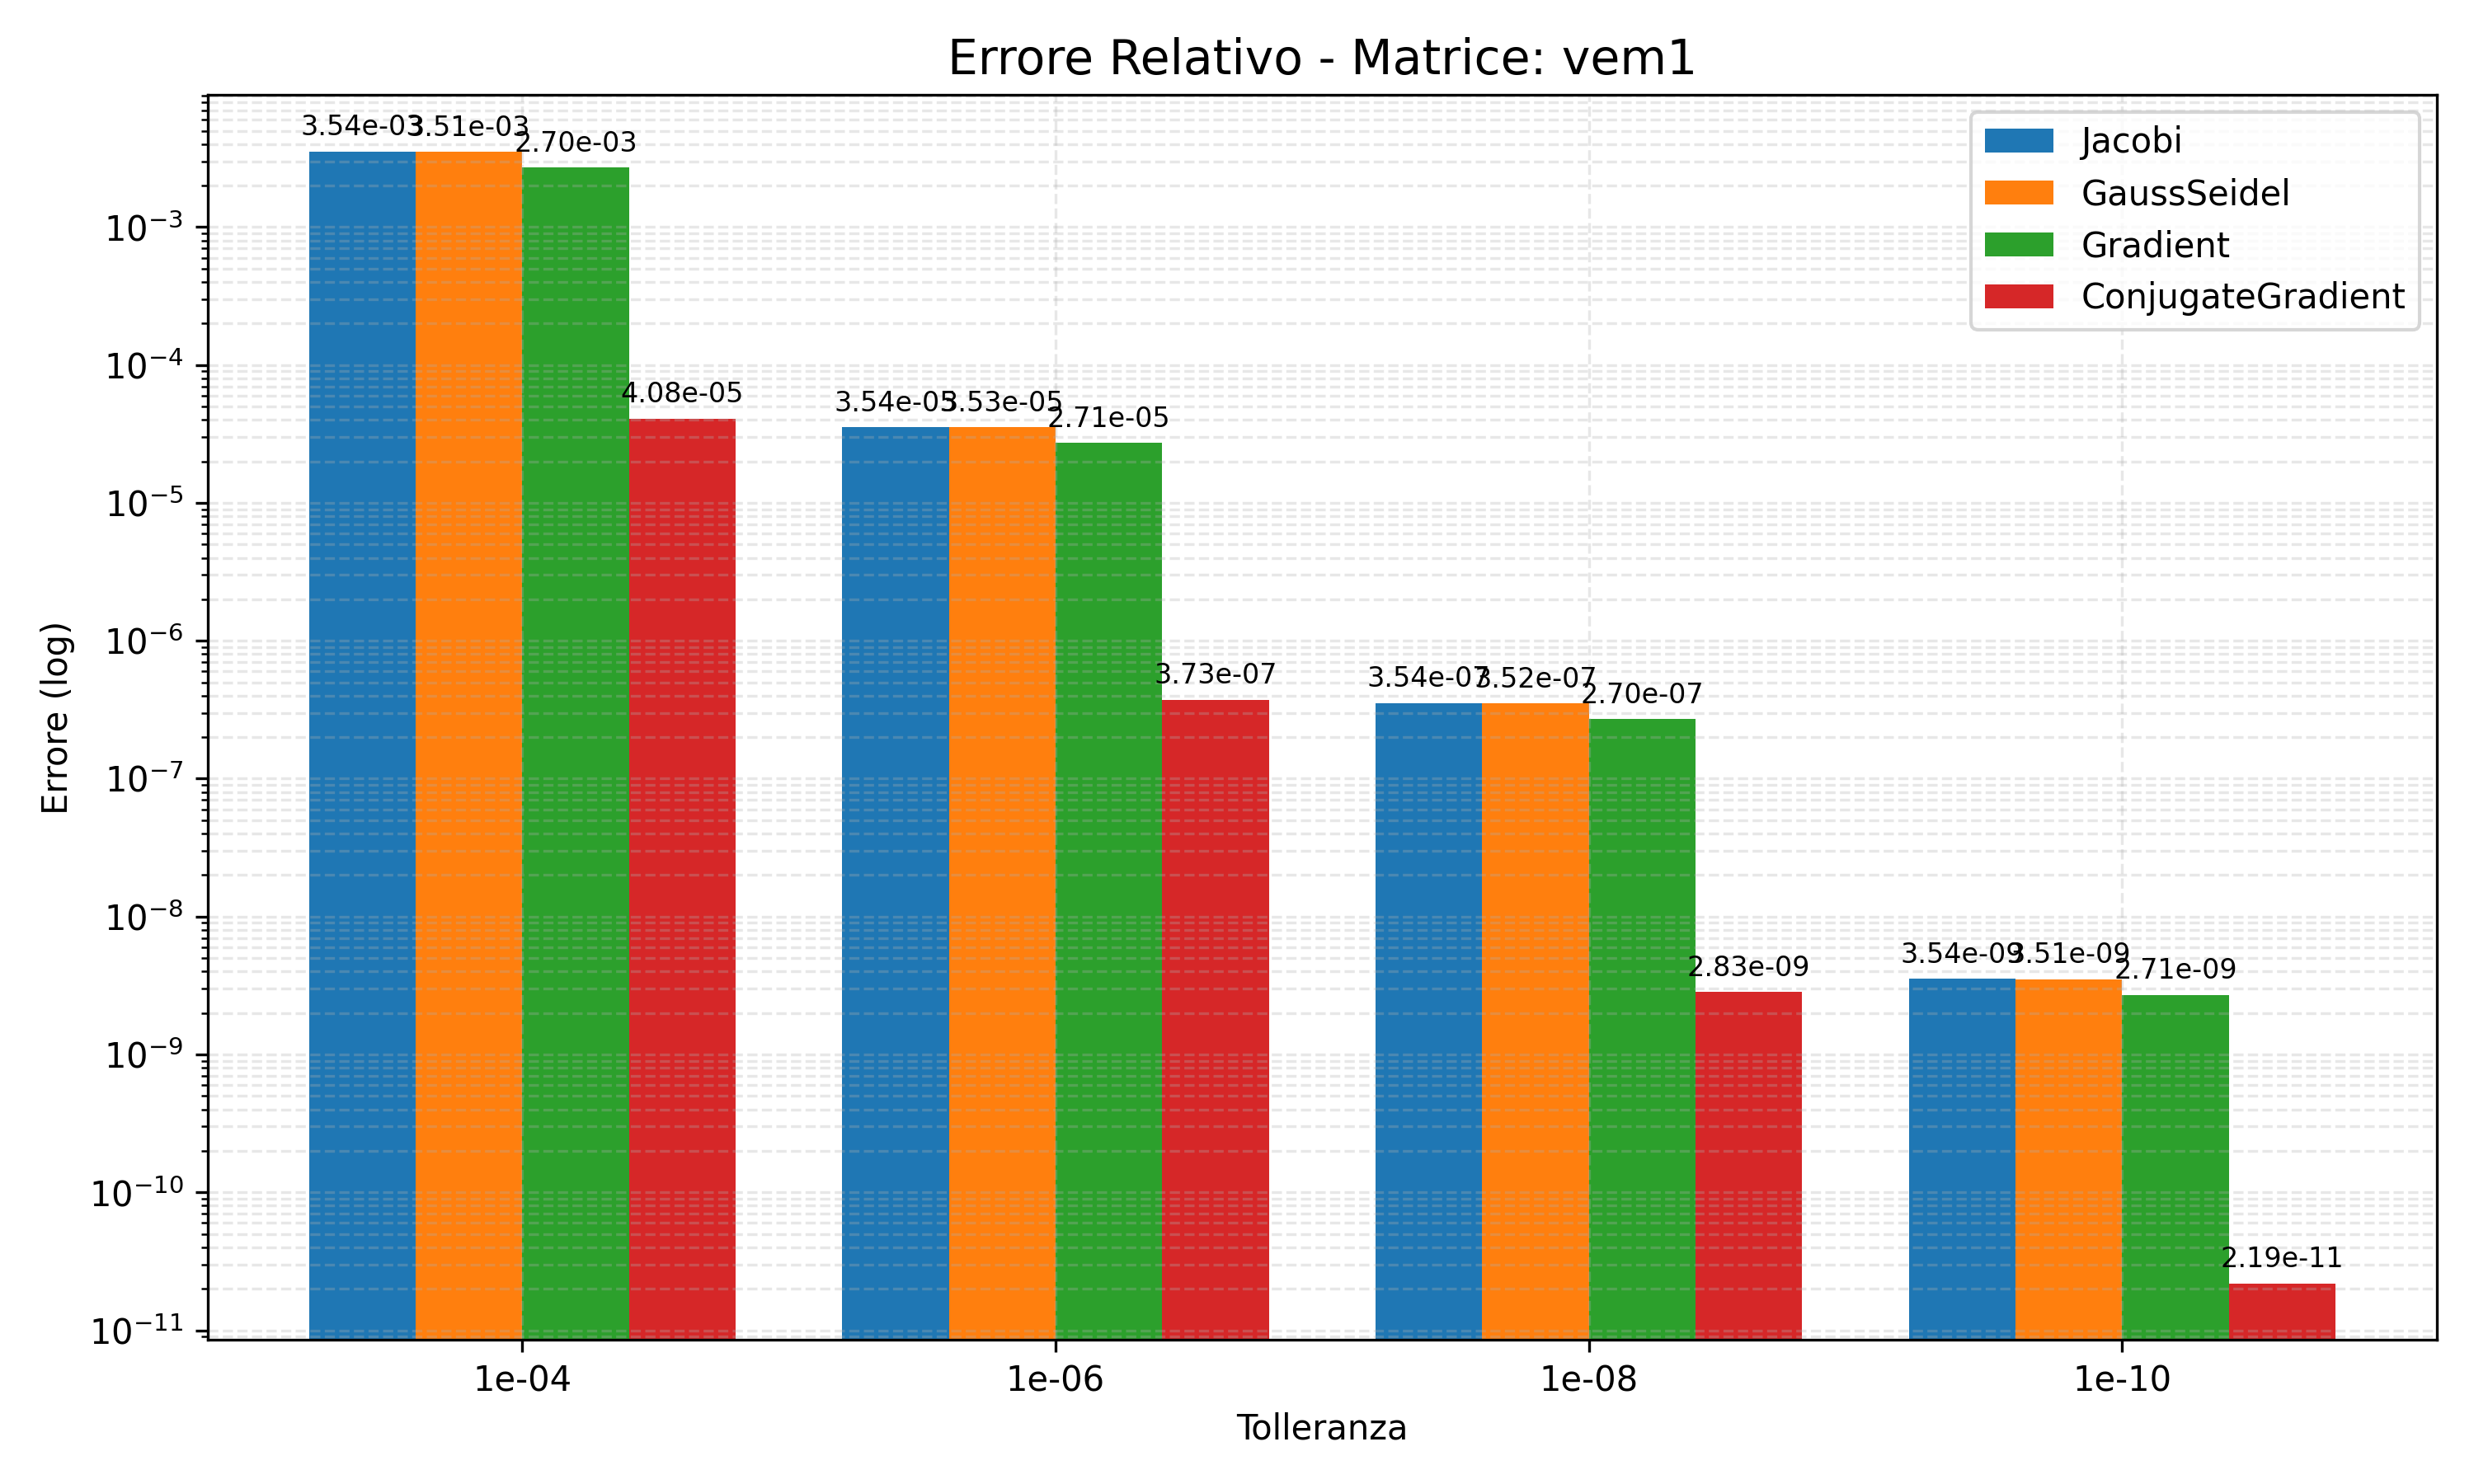
\includegraphics[width=0.9\textwidth]{plots/vem1_error.png}
    \caption{Errore relativo per vem1}
\end{figure}

A differenza delle matrici precedenti, \textbf{Jacobi}, \textbf{Gau\ss{}-Seidel} e il \textbf{Gradiente} standard mostrano valori di errore praticamente identici per ogni livello di tolleranza. Il \textbf{Gradiente Coniugato}, invece, si distingue nettamente dagli altri, infatti pur attestandosi su valori simili per tolleranze alte, raggiunge una precisione significativamente superiore al diminuire della soglia. Questo conferma i benefici del basso numero di condizionamento di \texttt{vem1} per questo metodo.

\section{Matrice: vem2}
\subsection{Analisi della Matrice}
In questa sottosezione viene presentata l'analisi morfologica della matrice \texttt{vem2}. La tabella \ref{tab:analisi_vem2} ne riassume le caratteristiche strutturali, mentre la figura \ref{fig:heatmap_vem2} ne mostra la distribuzione dei valori tramite heatmap.

\begin{figure}[H]
    \centering
    % Prima colonna per la tabella
    \begin{minipage}[c]{0.48\textwidth}
        \centering
        \begin{tabular}{lr}
            \toprule
            \multicolumn{2}{l}{\textbf{Matrice vem2}} \\
            \midrule
            \textbf{Rows} & 2601 \\
            \textbf{Cols} & 2601 \\
            \textbf{Area} & 6765201 \\
            \textbf{Density (\%)} & 0.314 \\
            \textbf{Mean} & 0.0186 \\
            \textbf{Std Dev} & 1.08 \\
            \textbf{Condition Number} & 507.0 \\
            \bottomrule
        \end{tabular}
        \captionof{table}{Analisi vem2}
        \label{tab:analisi_vem2}
    \end{minipage}\hfill
    % Seconda colonna per l'immagine
    \begin{minipage}[c]{0.48\textwidth}
        \centering
        \includegraphics[width=\linewidth]{plots/vem2_heatmap.png}
        \captionof{figure}{Heatmap di vem2}
        \label{fig:heatmap_vem2}
    \end{minipage}
\end{figure}

La matrice \texttt{vem2} è la più sparsa dell'intero set, con una densità dello 0.31\%. Il suo numero di condizionamento (507.0) è leggermente superiore rispetto a \texttt{vem1}, ma rimane comunque basso, rendendo questa matrice altrettanto favorevole per tutti i metodi iterativi analizzati.

\subsection{Risultati Numerici}
La seguente tabella riassume i risultati ottenuti per i quattro algoritmi al variare della tolleranza richiesta per la matrice \texttt{vem2}.

\begin{table}[H]
    \centering
    \begin{tabular}{|c|c|c|c|c|}
        \hline
        \textbf{Tol} & \textbf{Metodo} & \textbf{Numero iterazioni} & \textbf{Tempo (s)} & \textbf{Errore relativo} \\
        \hline
        $10^{-4}$ & Jacobi & 1927 & 0.0585 & $4.97 \cdot 10^{-3}$ \\
                  & Gauss-Seidel & 965 & 4.0953 & $4.95 \cdot 10^{-3}$ \\
                  & Gradient & 1308 & 0.0380 & $3.81 \cdot 10^{-3}$ \\
                  & Conjugate Gradient & 47 & 0.0021 & $5.73 \cdot 10^{-5}$ \\
        \hline
        $10^{-6}$ & Jacobi & 3676 & 0.0942 & $4.97 \cdot 10^{-5}$ \\
                  & Gauss-Seidel & 1840 & 7.4654 & $4.94 \cdot 10^{-5}$ \\
                  & Gradient & 2438 & 0.0614 & $3.79 \cdot 10^{-5}$ \\
                  & Conjugate Gradient & 56 & 0.0016 & $4.74 \cdot 10^{-7}$ \\
        \hline
        $10^{-8}$ & Jacobi & 5425 & 0.1174 & $4.97 \cdot 10^{-7}$ \\
                  & Gauss-Seidel & 2714 & 10.8939 & $4.96 \cdot 10^{-7}$ \\
                  & Gradient & 3566 & 0.0898 & $3.81 \cdot 10^{-7}$ \\
                  & Conjugate Gradient & 66 & 0.0019 & $4.30 \cdot 10^{-9}$ \\
        \hline
        $10^{-10}$ & Jacobi & 7174 & 0.1560 & $4.96 \cdot 10^{-9}$ \\
                  & Gauss-Seidel & 3589 & 14.3936 & $4.95 \cdot 10^{-9}$ \\
                  & Gradient & 4696 & 0.1180 & $3.80 \cdot 10^{-9}$ \\
                  & Conjugate Gradient & 74 & 0.0021 & $2.25 \cdot 10^{-11}$ \\
        \hline
    \end{tabular}
    \caption{Risultati numerici per vem2}
\end{table}

\subsection{Analisi delle Iterazioni}
\begin{figure}[H]
    \centering
    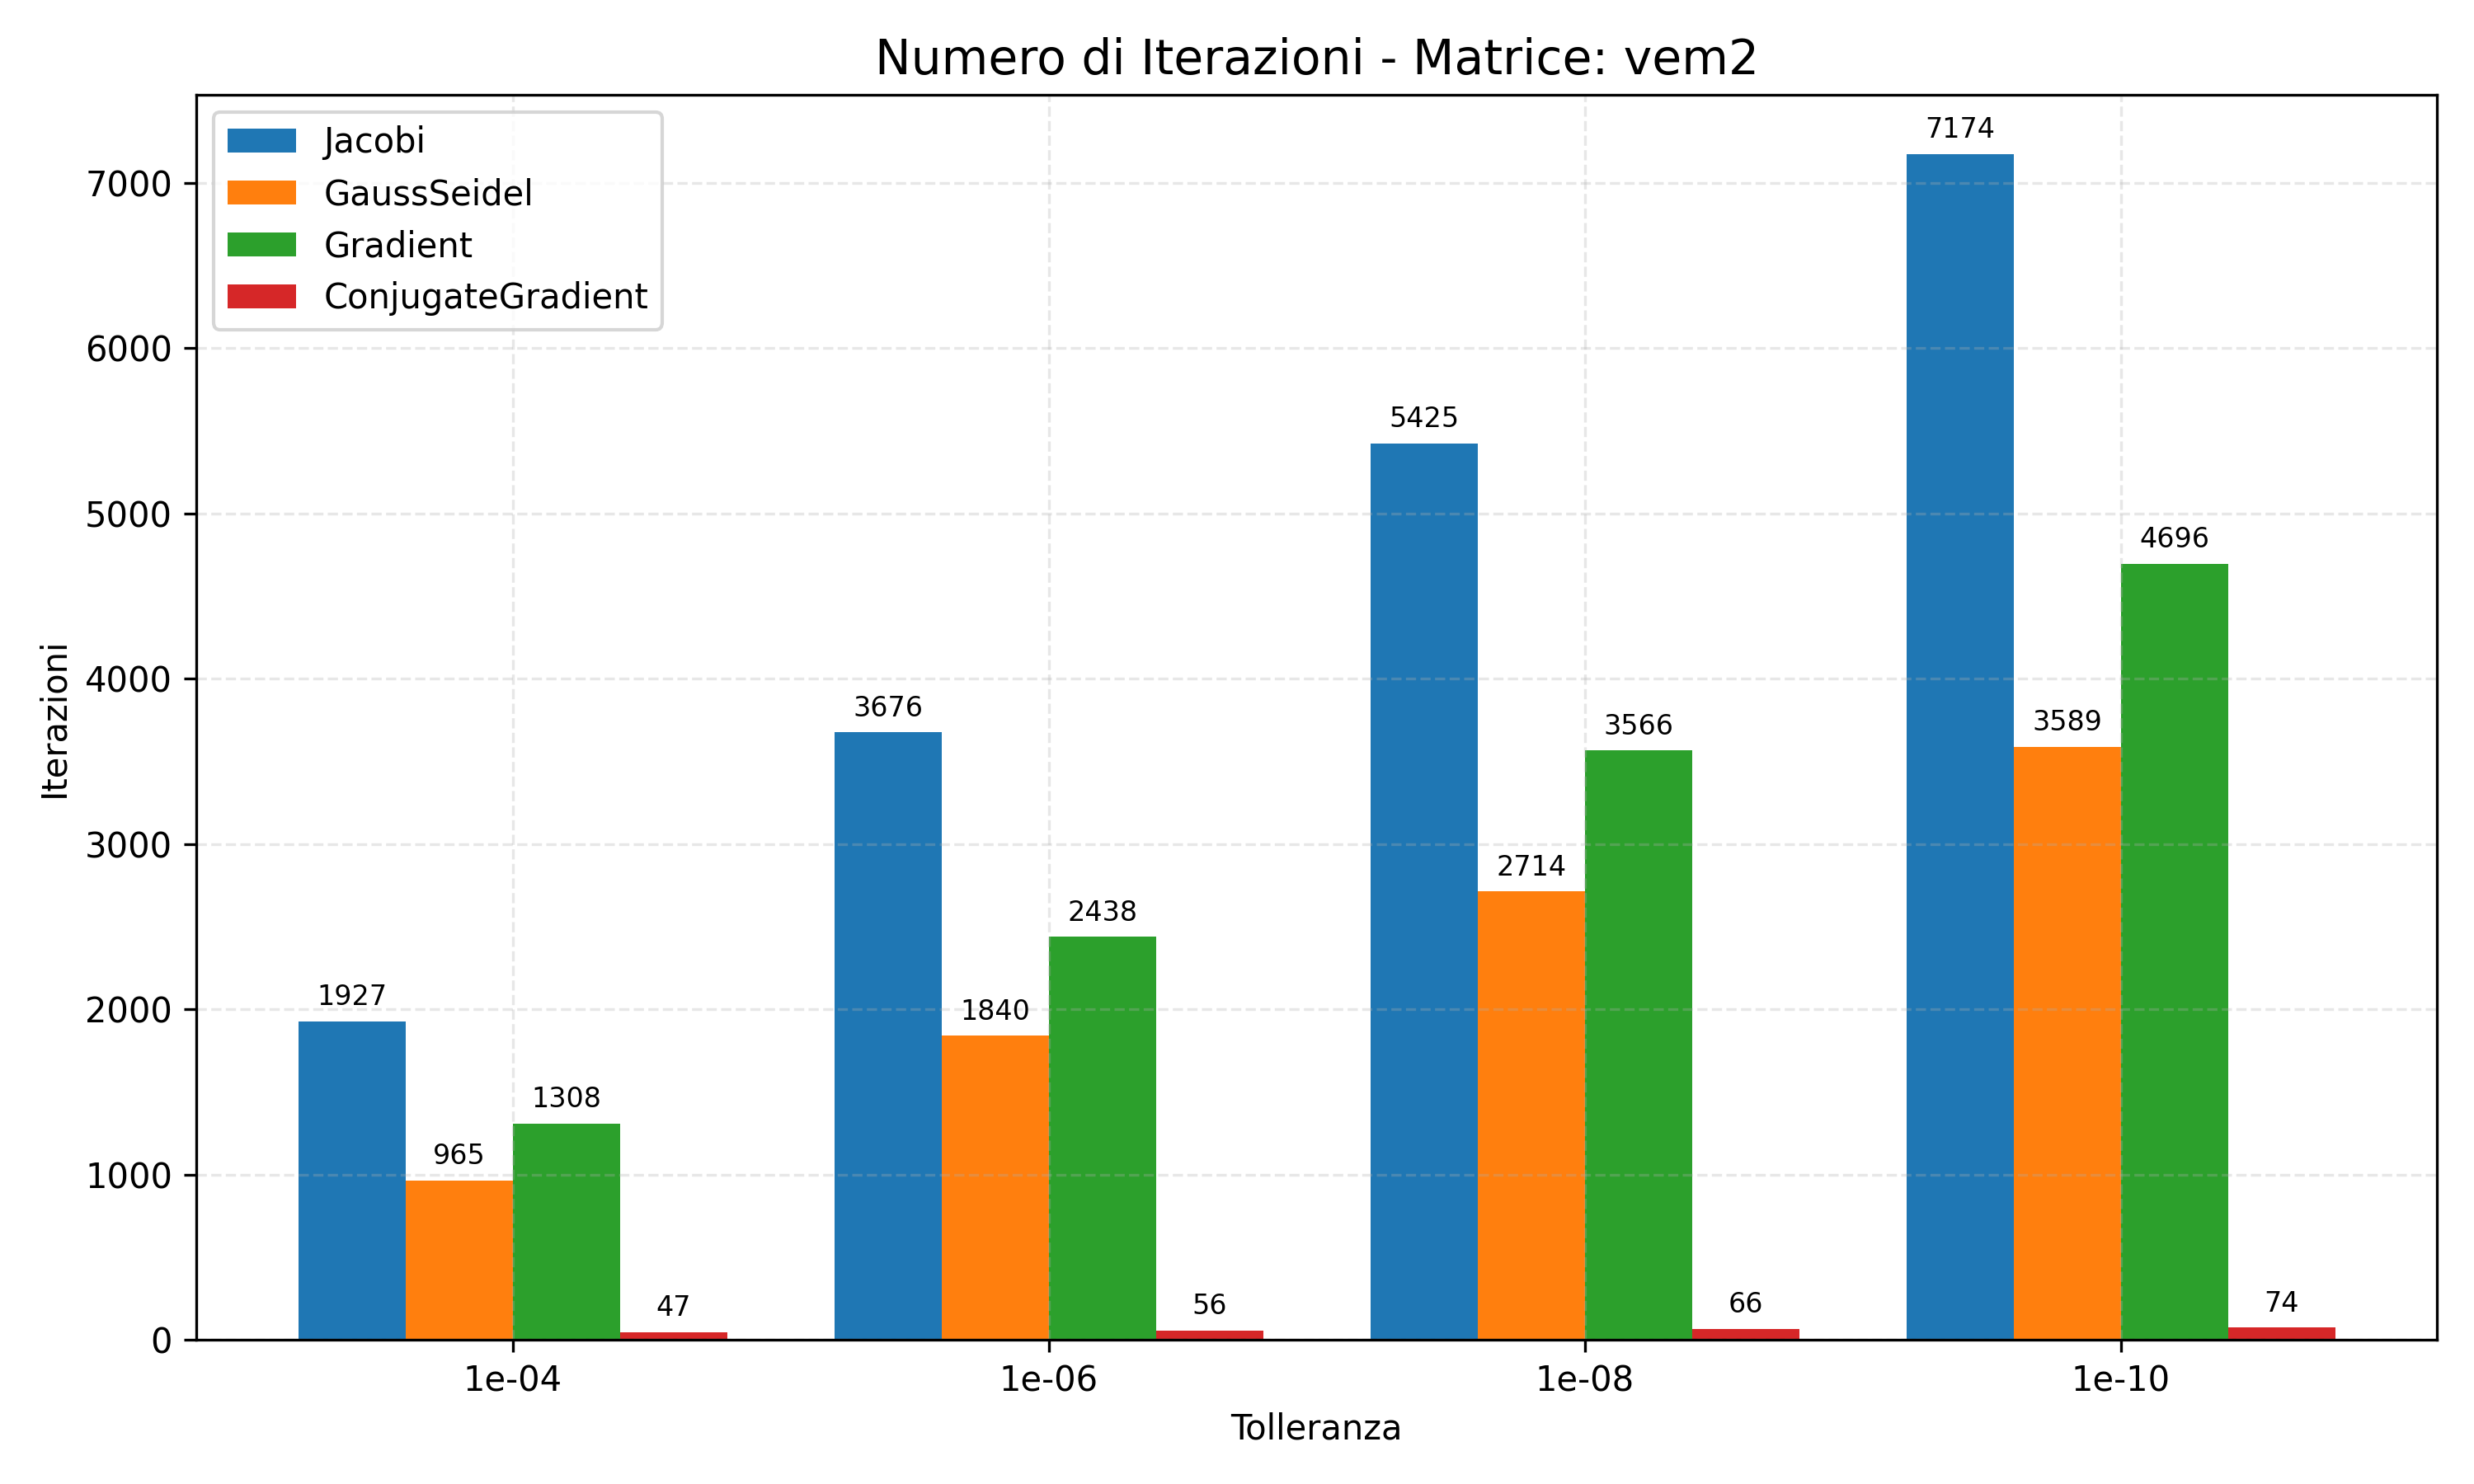
\includegraphics[width=0.9\textwidth]{plots/vem2_iterations.png}
    \caption{Numero di iterazioni per vem2}
\end{figure}

Per la matrice \texttt{vem2}, l'andamento delle iterazioni rispecchia quanto già osservato per \texttt{vem1}. Il \textbf{Gradiente Coniugato} si conferma il più efficiente in assoluto, convergendo in pochissimi passi. \textbf{Jacobi} risulta nuovamente il metodo più lento, richiedendo il maggior numero di iterazioni per ogni livello di tolleranza. Sempre come per la matrice precedente inoltre, \textbf{Gau\ss{}-Seidel} e il \textbf{Gradiente} si mantengono su valori intermedi, con Gau\ss{}-Seidel che converge con un numero di passi costantemente inferiore.

\subsection{Analisi dei Tempi}
\begin{figure}[H]
    \centering
    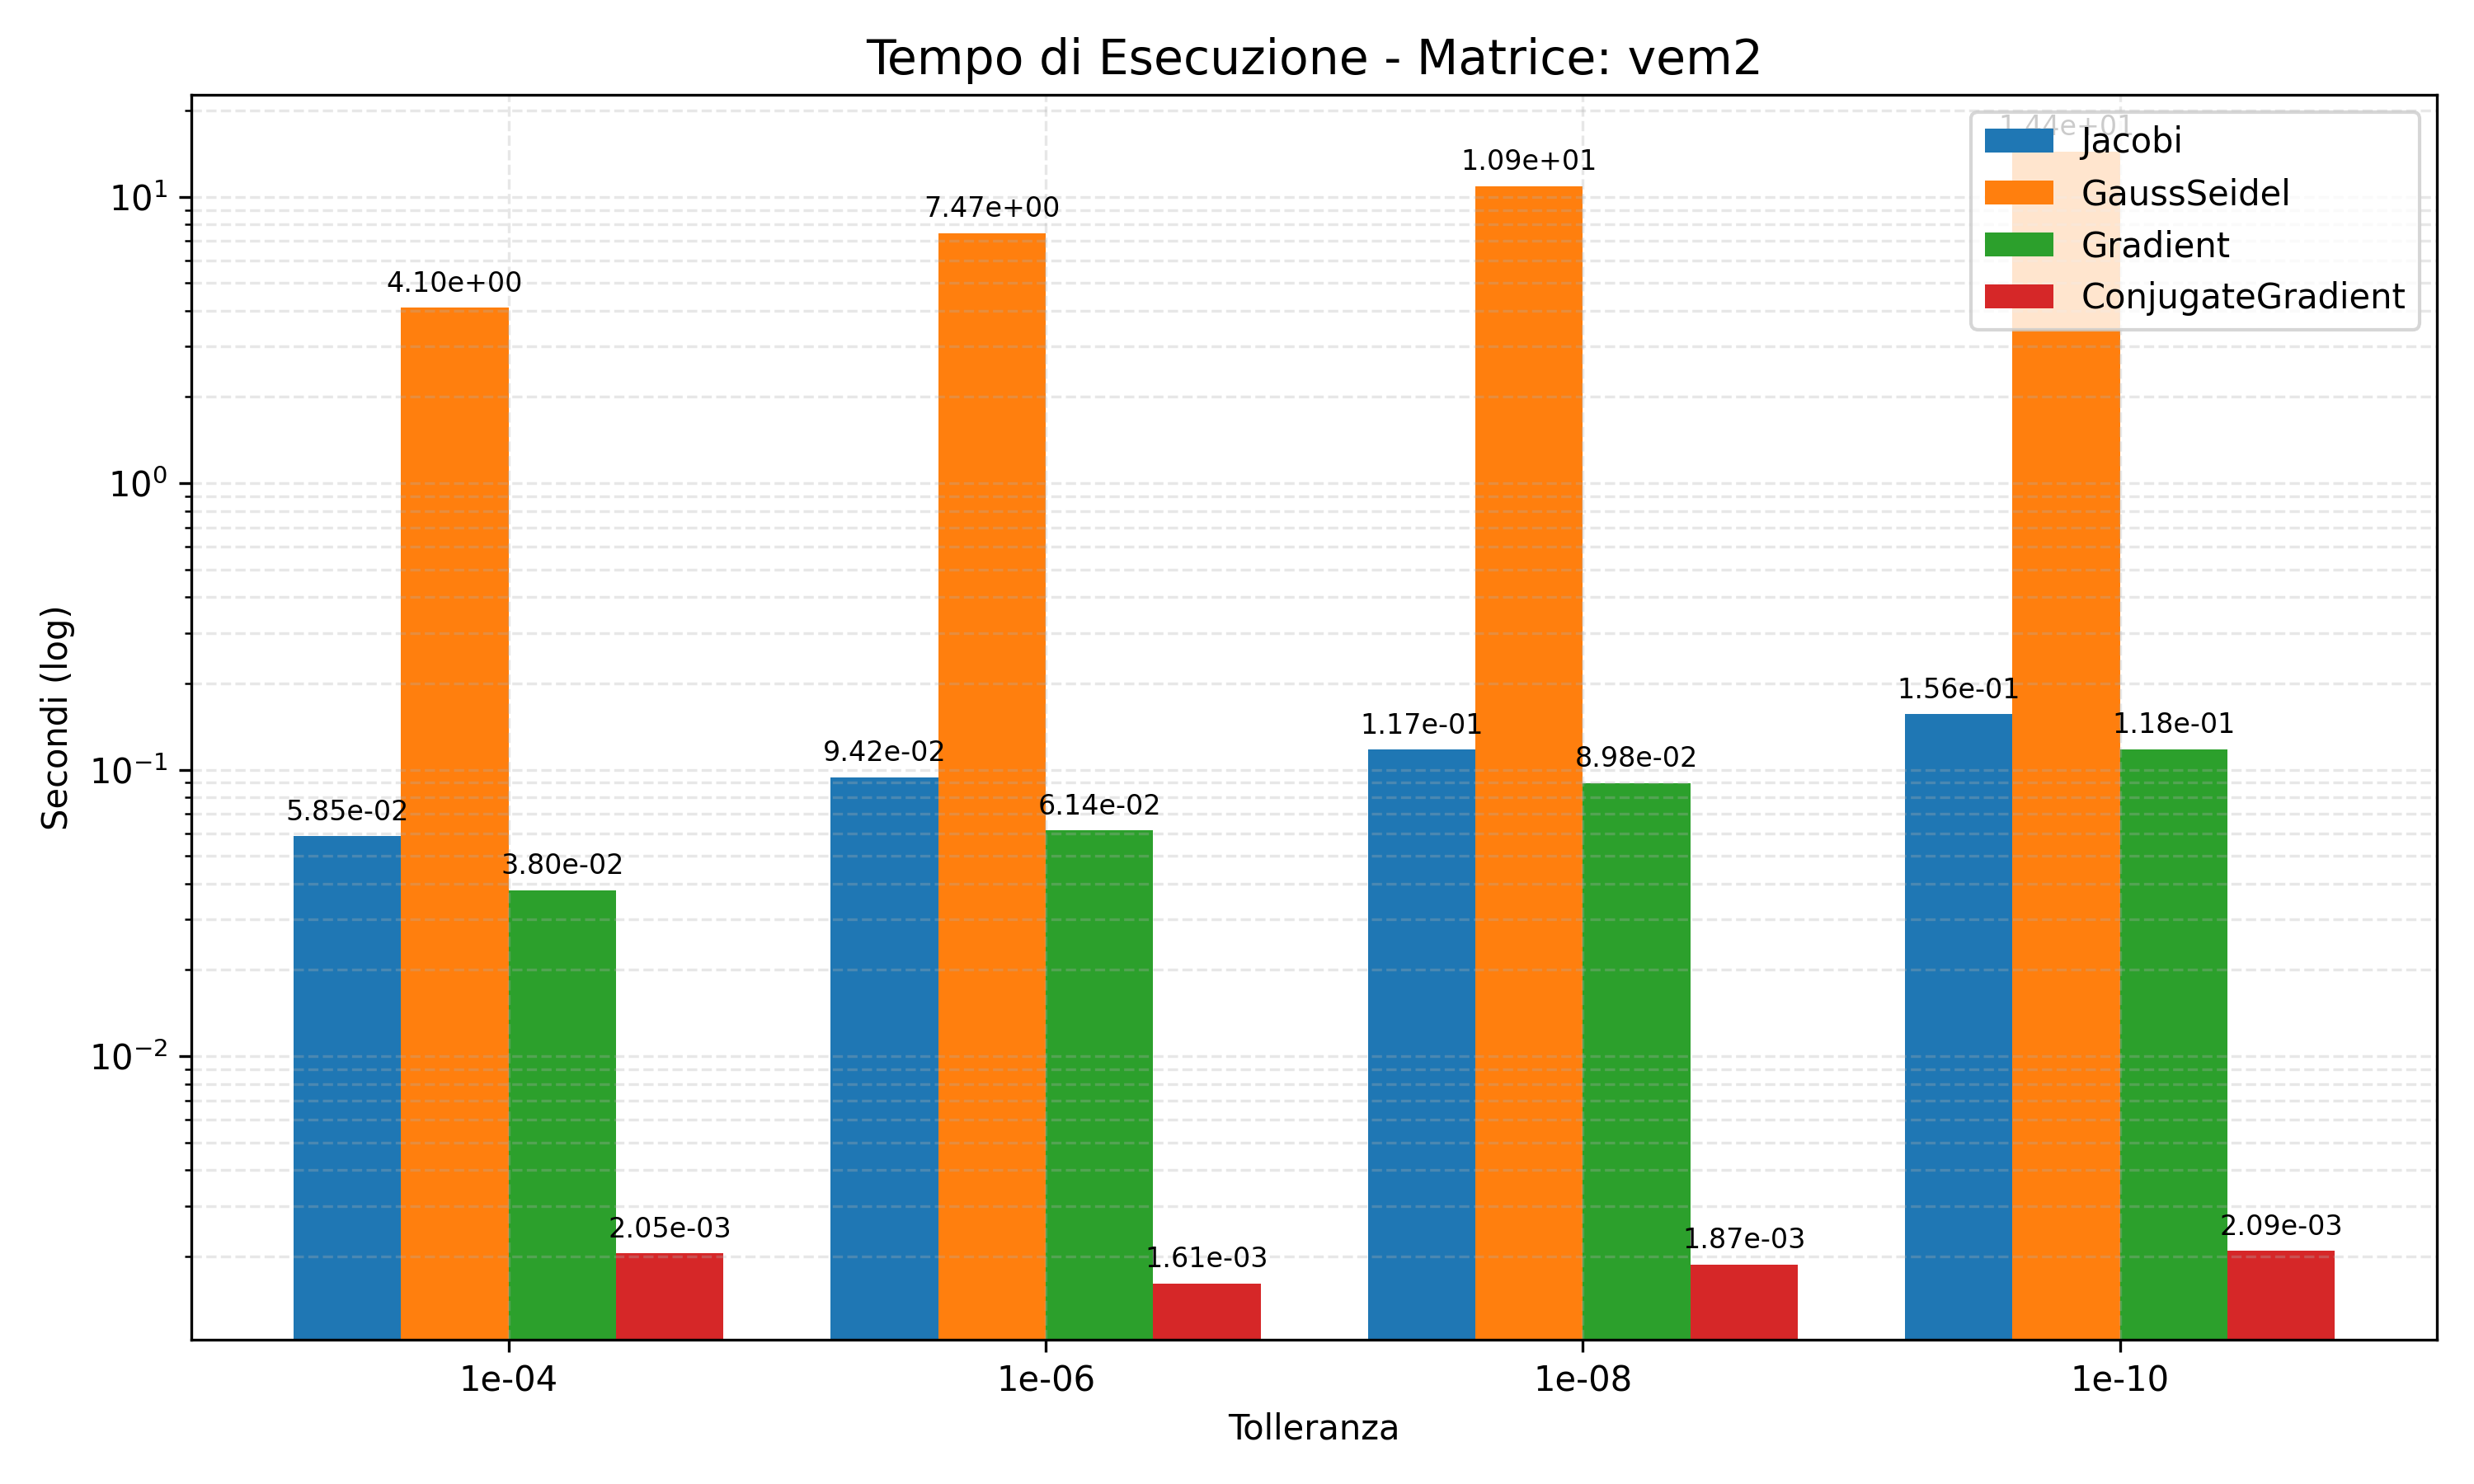
\includegraphics[width=0.9\textwidth]{plots/vem2_time.png}
    \caption{Tempo di esecuzione per vem2}
\end{figure}

Il \textbf{Gradiente Coniugato} si conferma l'algoritmo più veloce in assoluto, completando l'esecuzione in pochi millisecondi. \textbf{Jacobi} e il \textbf{Gradiente} seguono a distanza ravvicinata, mentre \textbf{Gau\ss{}-Seidel} risulta di gran lunga il più lento, con tempi di esecuzione notevolmente superiori rispetto al \textbf{Gradiente Coniugato}.

\subsection{Confronto Implementazioni Gauß-Seidel}
\begin{figure}[H]
    \centering
    \begin{minipage}{0.48\textwidth}
        \centering
        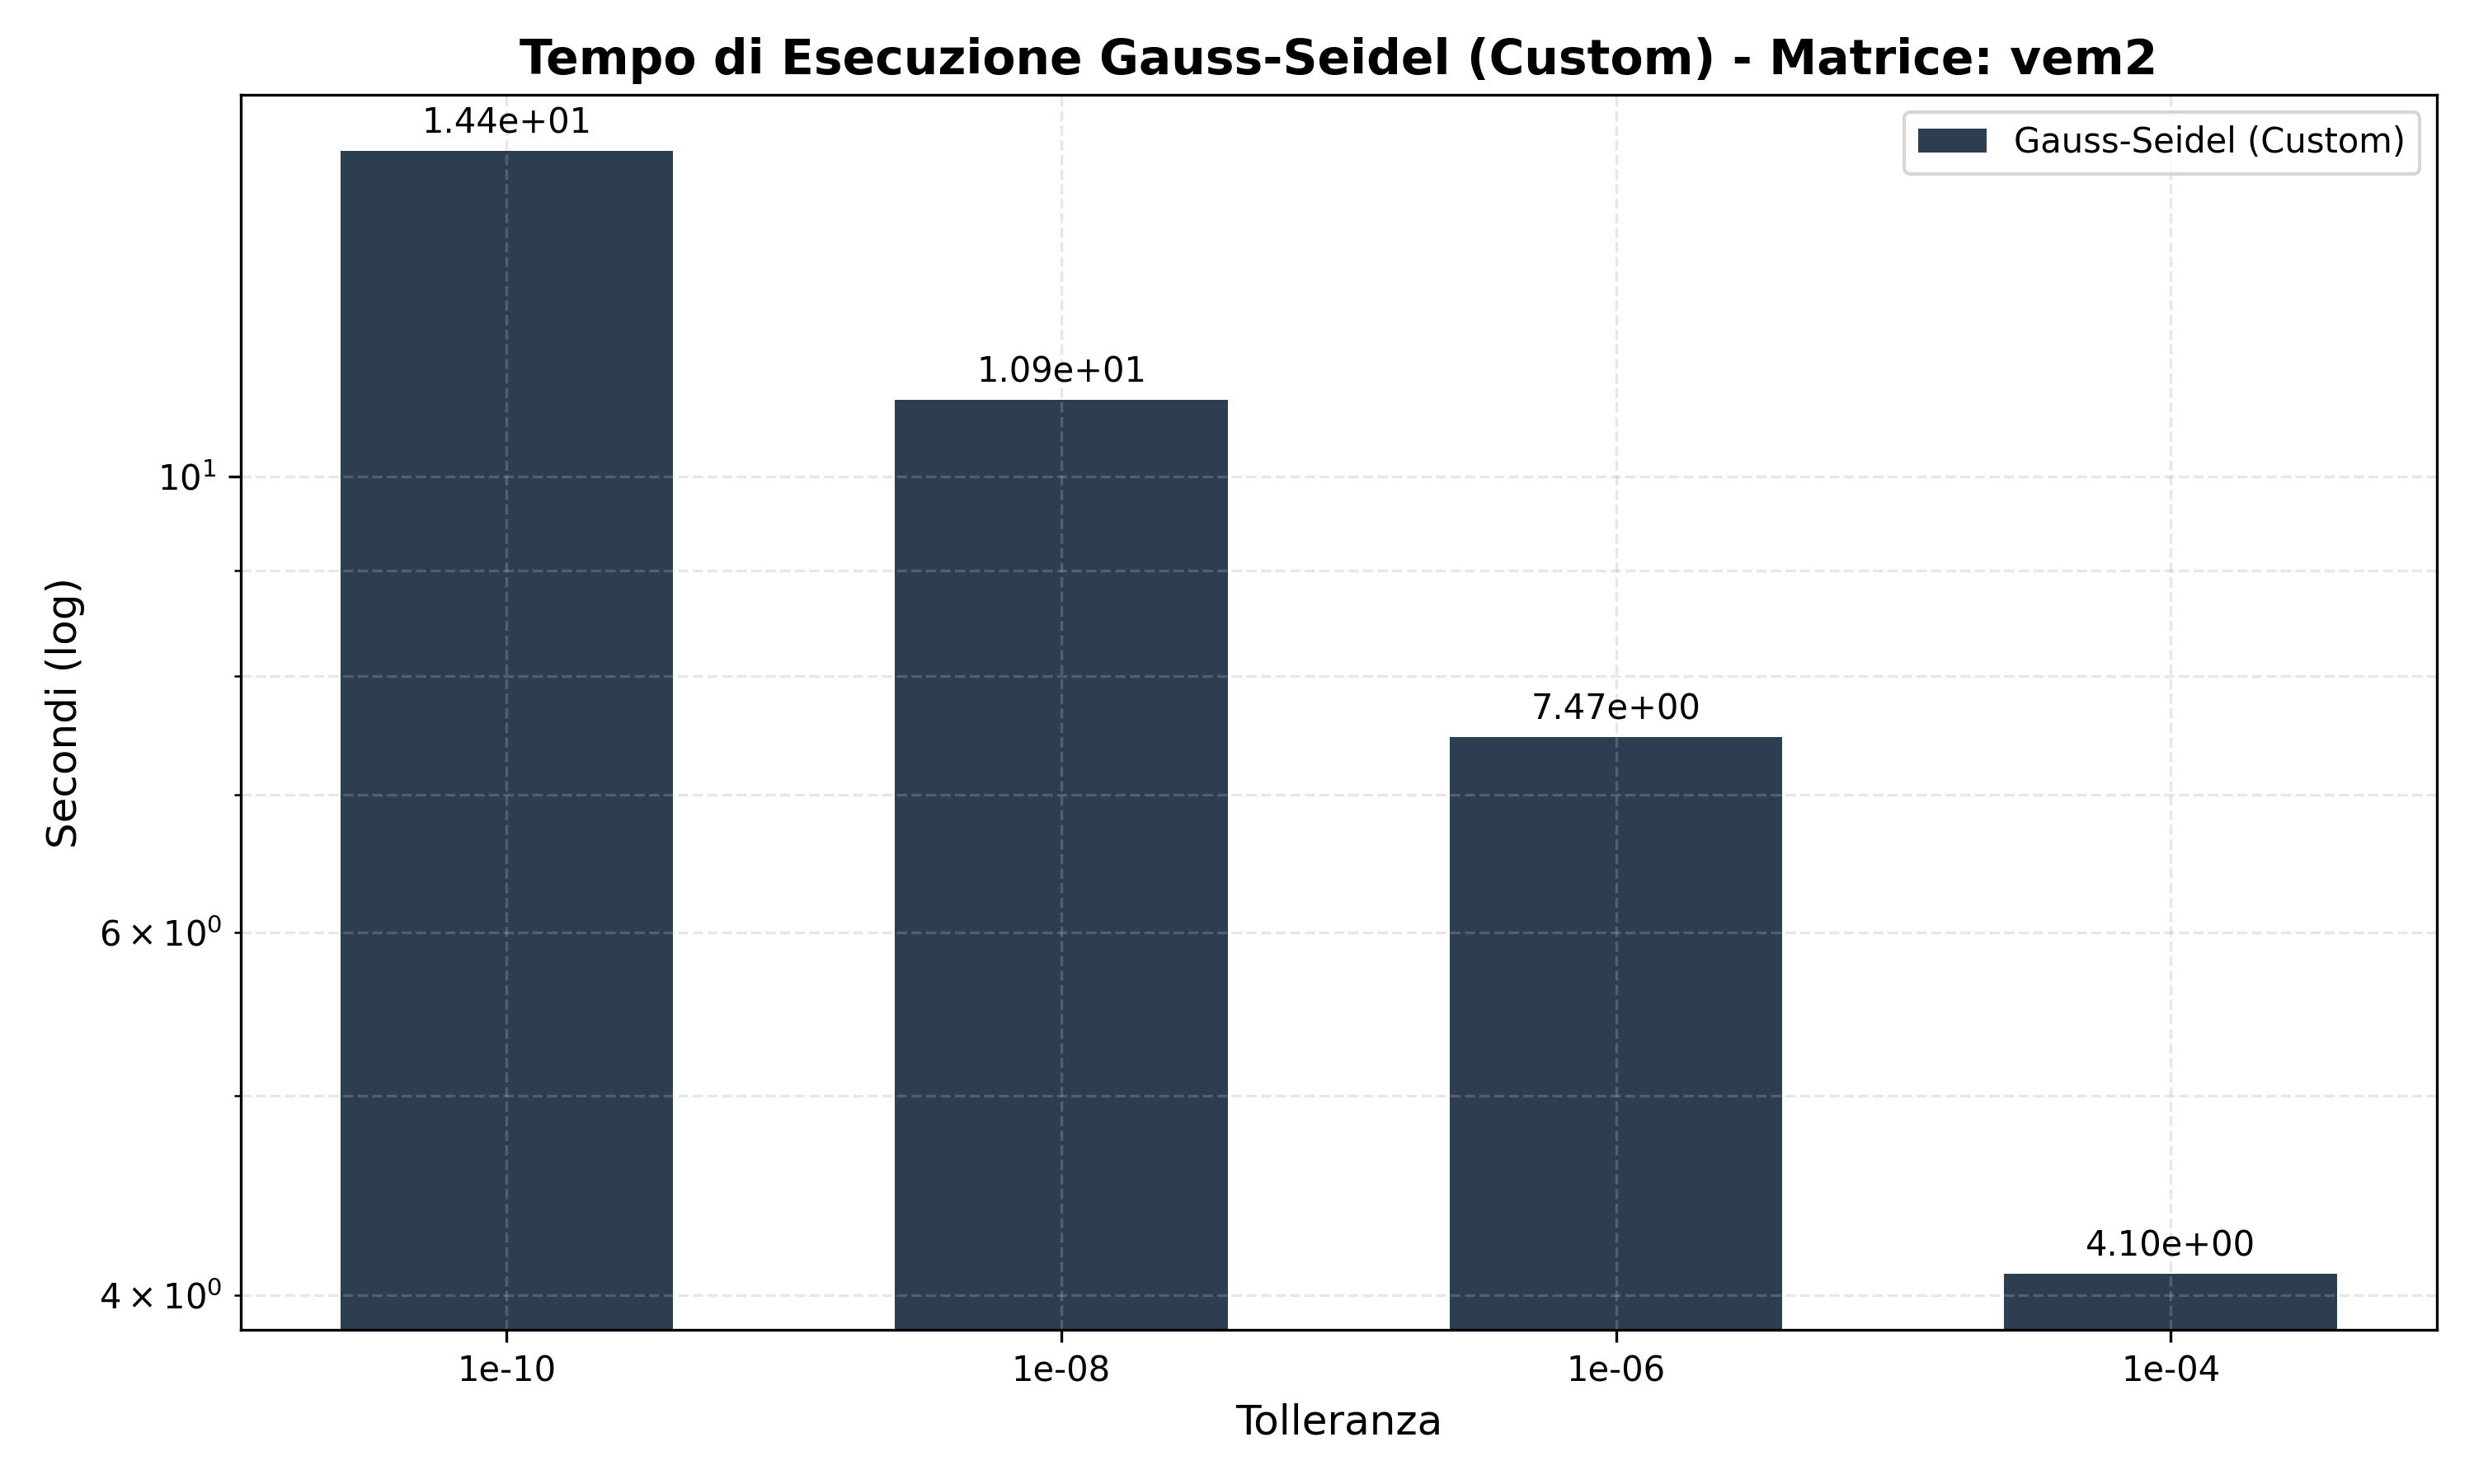
\includegraphics[width=\textwidth]{plots/gs_custom_vem2.png} % Da sostituire
        \caption{GS Custom (Forward Sub)}
    \end{minipage}\hfill
    \begin{minipage}{0.48\textwidth}
        \centering
        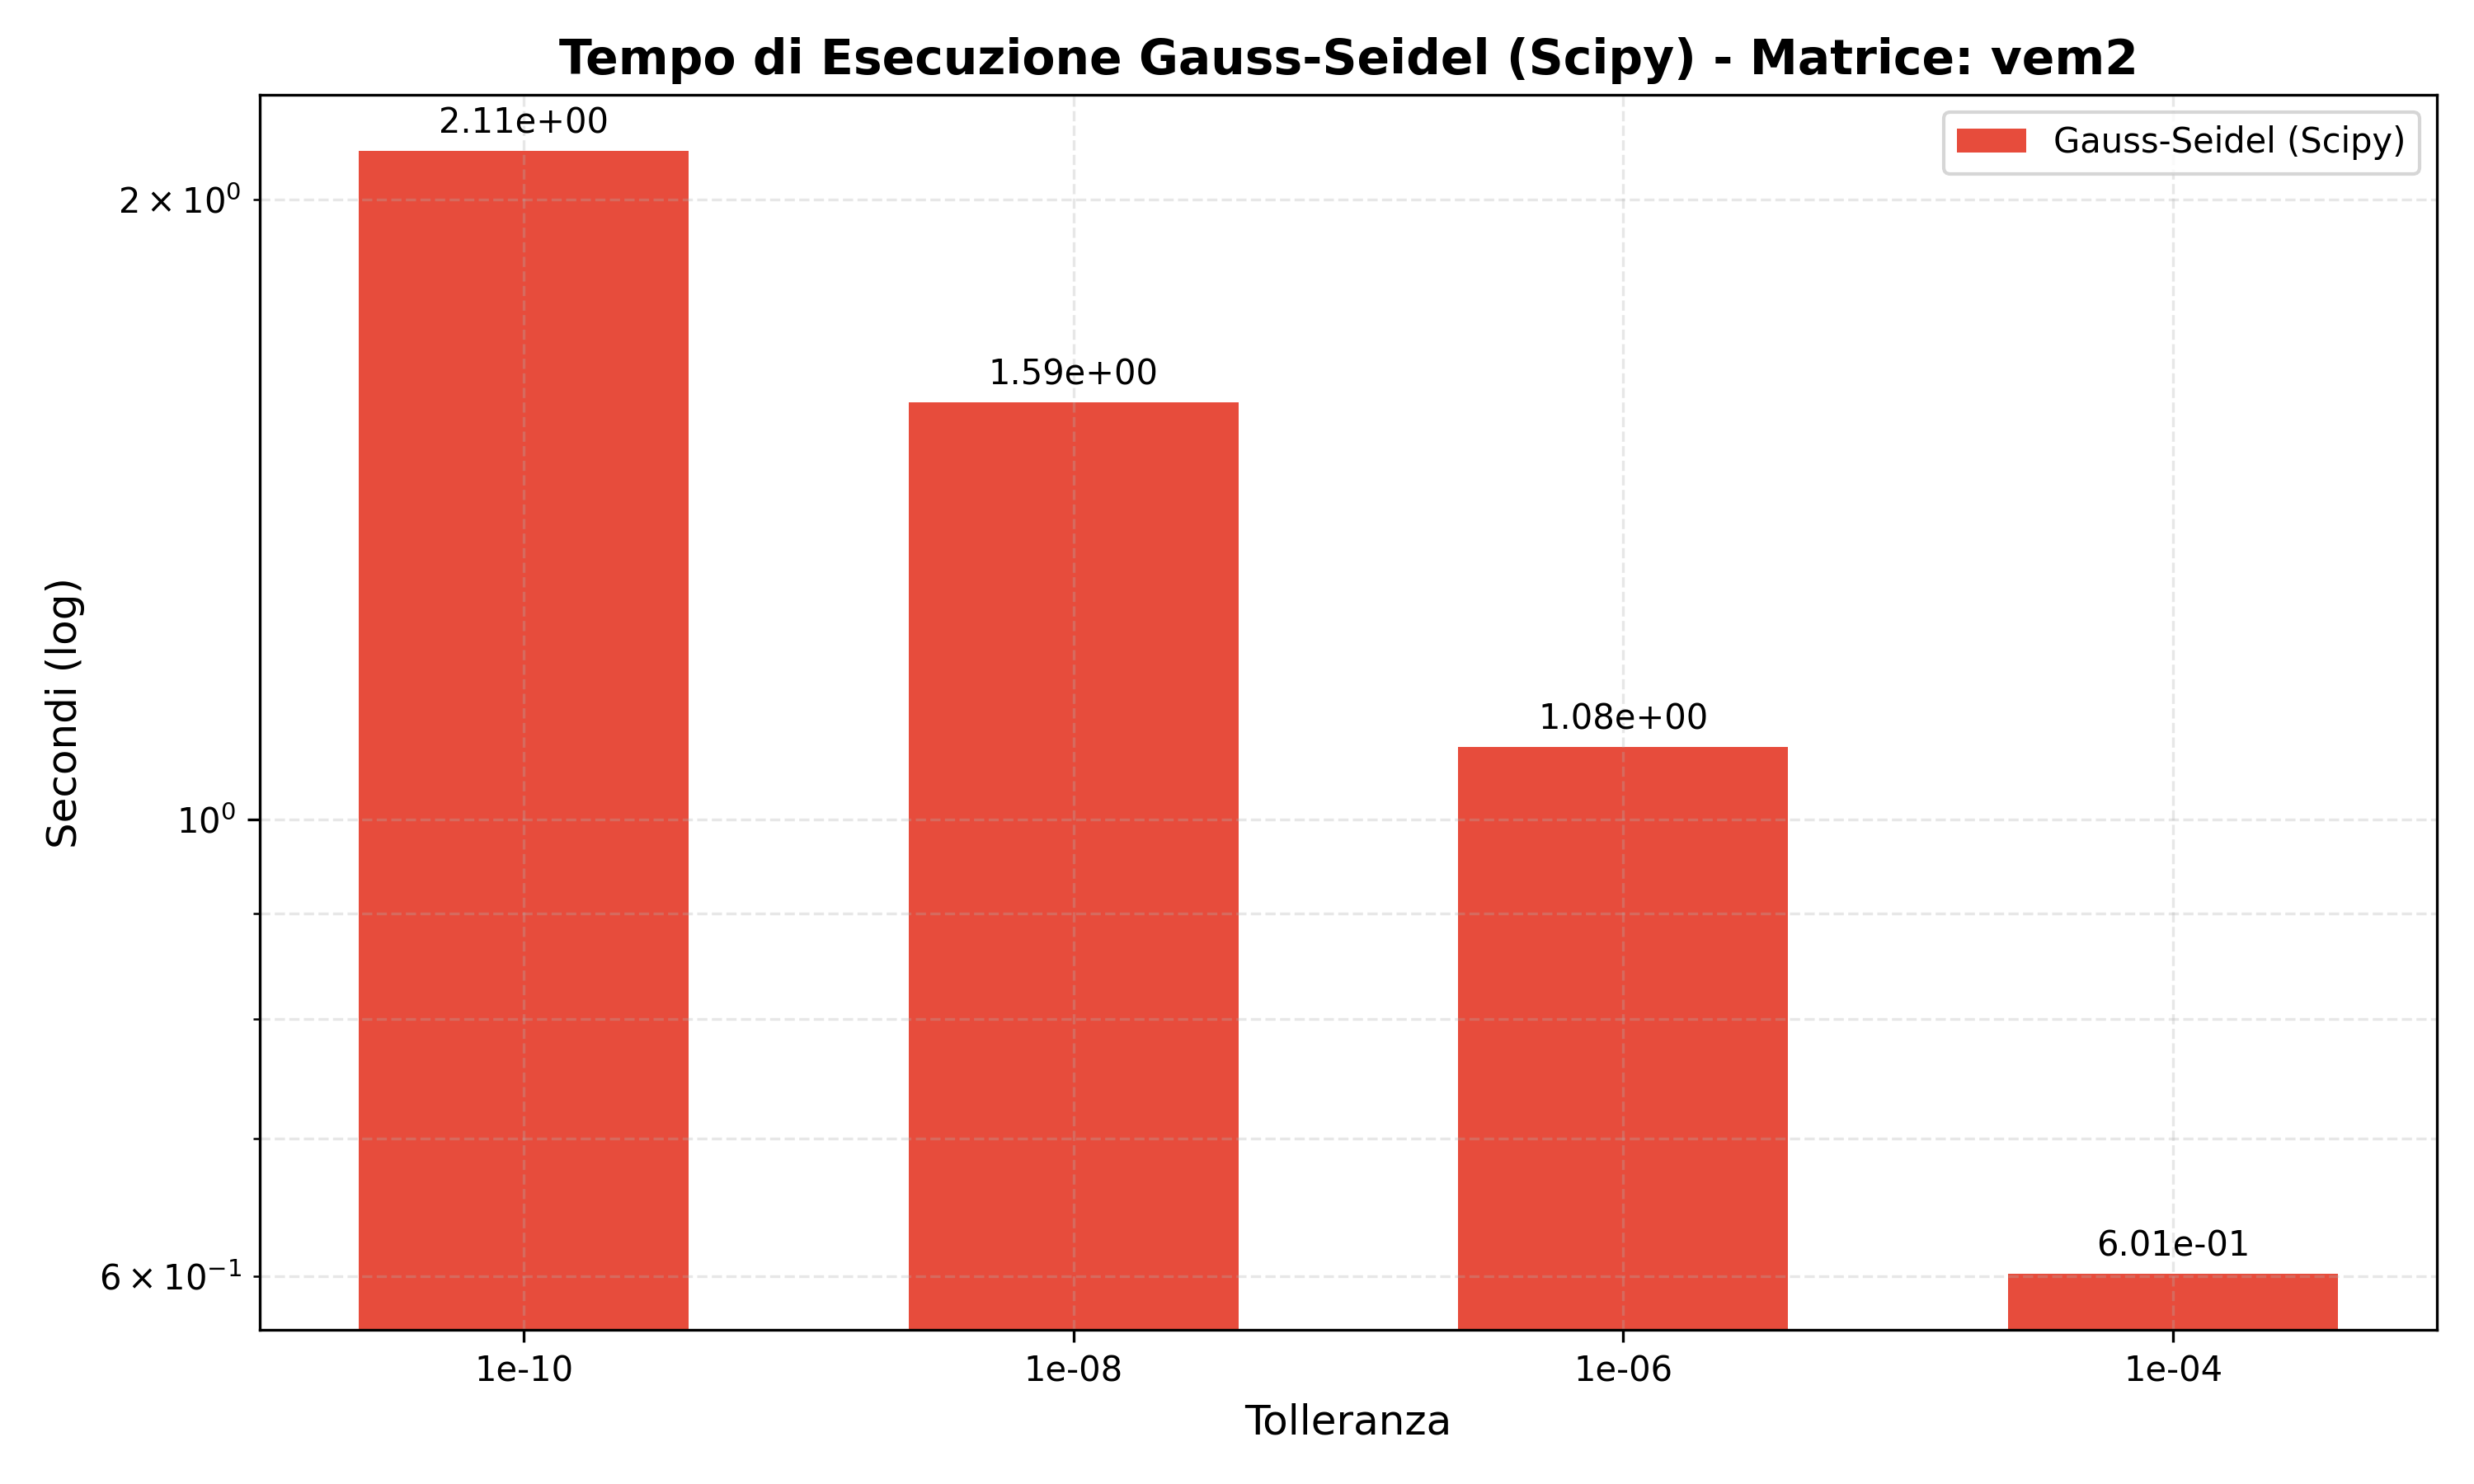
\includegraphics[width=\textwidth]{plots/gs_scipy_vem2.png} % Da sostituire
        \caption{GS SciPy (spsolve\_triangular)}
    \end{minipage}
\end{figure}

Come discusso nel capitolo precedente, è stato condotto un confronto diretto tra l'implementazione custom di sostituzione in avanti e la funzione ottimizzata in C offerta da SciPy (\texttt{spsolve\_triangular}). I grafici illustrano il tempo totale di esecuzione dell'algoritmo, e non quello della singola iterazione. A parità di iterazioni e di errore relativo, l'implementazione manuale mostra una notevole lentezza del loop nativo di Python rispetto alle funzioni pre-compilate della libreria.

\subsection{Analisi dell'Errore Relativo}
\begin{figure}[H]
    \centering
    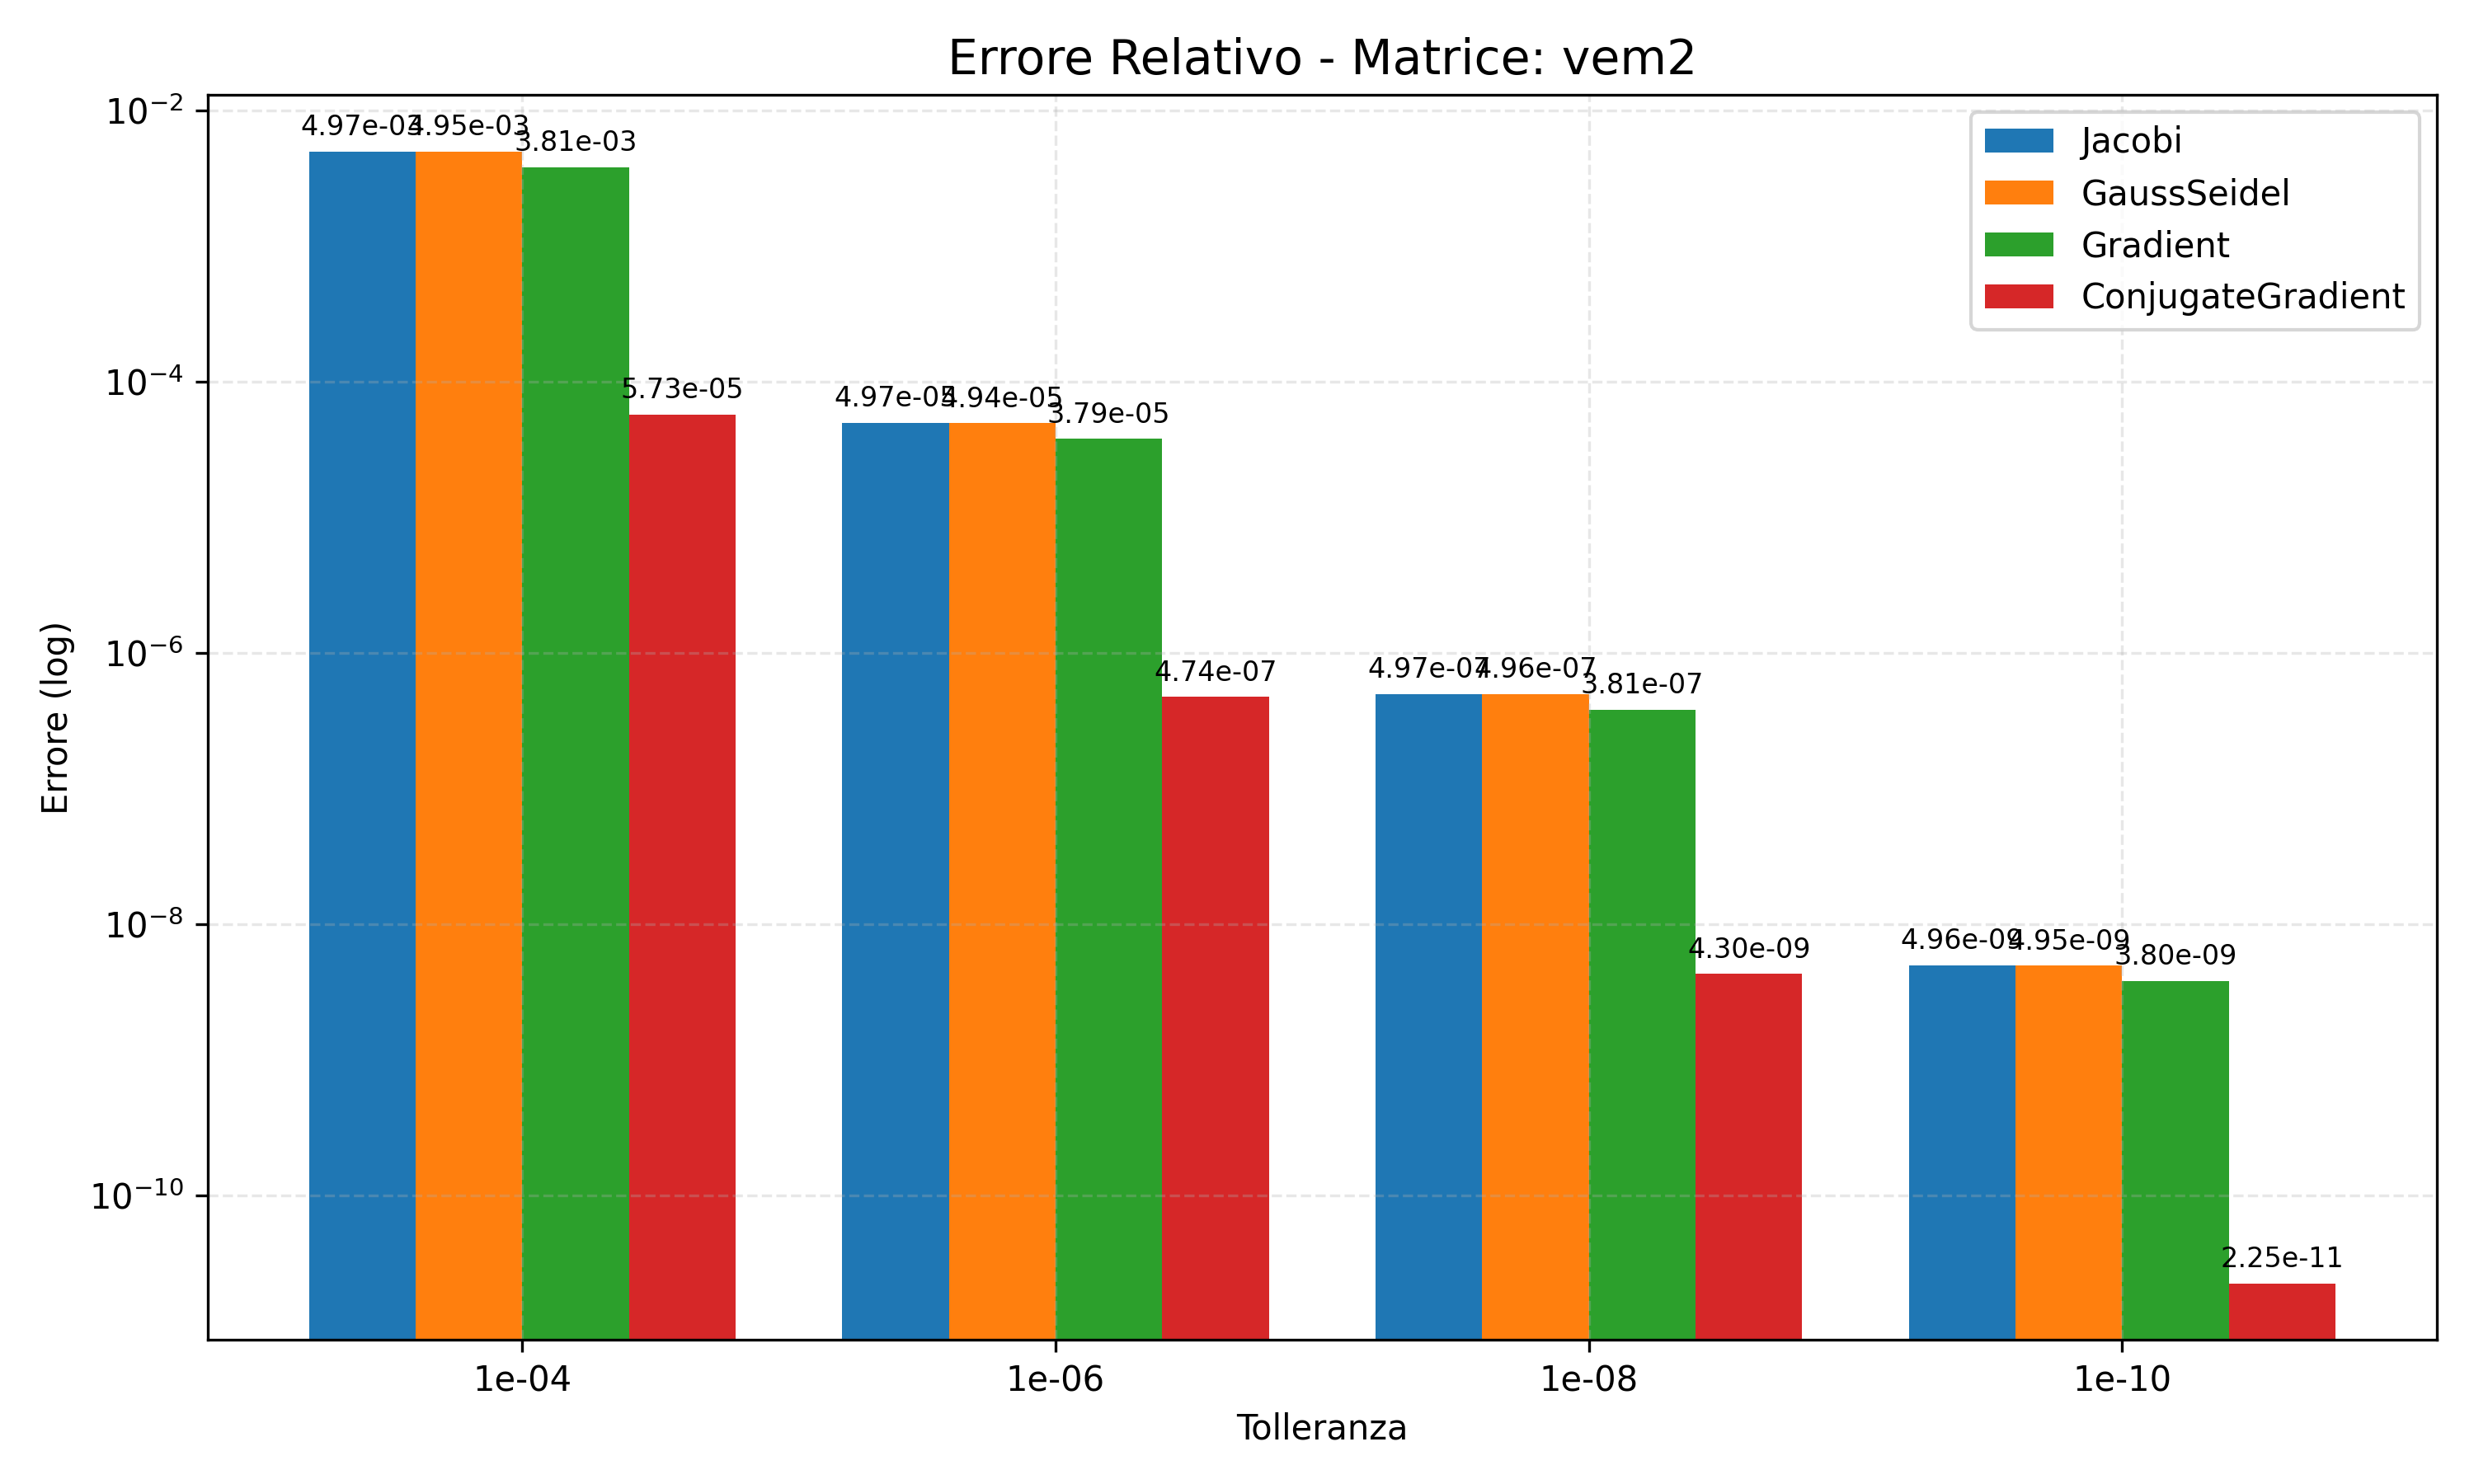
\includegraphics[width=0.9\textwidth]{plots/vem2_error.png}
    \caption{Errore relativo per vem2}
\end{figure}

Tutti i metodi soddisfano le tolleranze richieste decrescendo in modo costante. \textbf{Jacobi}, \textbf{Gau\ss{}-Seidel} e il \textbf{Gradiente} mostrano valori di errore praticamente identici per ogni livello di tolleranza. Il \textbf{Gradiente Coniugato} si distingue invece dagli altri per ogni soglia testata, raggiungendo una precisione significativamente superiore già alle tolleranze più alte e accentuando ulteriormente questo vantaggio al diminuire della soglia.


\chapter{Conclusioni}

I test condotti sulle quattro matrici hanno confermato quanto ci si aspettava dalla teoria, facendo emergere una gerarchia abbastanza chiara tra i metodi:

\begin{itemize}
    \item \textbf{Gradiente Coniugato:} È il metodo che si comporta meglio in quasi tutti gli scenari. Converge in pochissime iterazioni, è il più veloce in termini di tempo e raggiunge i valori di errore relativo più bassi. Il vantaggio è particolarmente evidente sulle matrici \texttt{vem}, dove il basso numero di condizionamento ne esalta ulteriormente le prestazioni.
    \item \textbf{Jacobi:} La sua struttura completamente vettorializzabile lo ha reso molto reattivo in termini di tempo. Sulle matrici \texttt{spa} si attesta su valori intermedi, mentre sulle \texttt{vem} diventa il più lento in assoluto per numero di iterazioni.
    \item \textbf{Gau\ss{}-Seidel:} Converge con il minor numero di iterazioni sulle matrici \texttt{spa}, ma i suoi tempi di esecuzione sono tra i più alti. Un colpevole è sicuramente la funzione \textit{custom} per la risoluzione del sistema triangolare inferiore, che è risultata dai test effettuati notevolmente più lenta rispetto al metodo nativo della libreria SciPy.
    \item \textbf{Gradiente:} E' risultato il metodo meno efficiente del gruppo, infatti ha richiesto un numero di iterazioni molto elevato su tutte le matrici, accumulando migliaia di passi a causa dell'avanzamento lento e ridondante verso il minimo.
\end{itemize}

\noindent In conclusione, la scelta del metodo dipende fortemente dalle caratteristiche della matrice, come la densità e il numero di condizionamento. Il Gradiente Coniugato si è rivelato il più efficiente nella maggior parte dei casi, ma conoscere la struttura del problema rimane fondamentale per scegliere l'algoritmo più adatto e ottenere le migliori prestazioni possibili.

\end{document}
